% !TeX program = xelatex
% !TeX encoding = UTF-8
% !TeX spellcheck = en_US
% !BIB program = biber
%% 
%% The above lines help editors like TeXstudio to automatically choose the right tools
%% to compile your LaTeX source file. If your tool does not support these magic comments,
%% you will need to make appropriate manual choices.
%% 
%% You can safely use "pdflatex" instead of "xelatex" if you prefer the pdfLaTeX toolchain.
%% However, pdfLaTeX will not be able to deliver the professional font experience that you
%% will get with XeLaTeX. You can also safely use "lualatex" instead of "xelatex" while
%% preserving the professional font experience if you prefer the LuaLaTeX toolchain.
%% 
%% _Important_: These magic comments should be on the first lines of your source file.
%% 
%%%%%%%%%%%%%%%%%%%%%%%%%%%%%%%%%%%%%%%%%%%%%%%%%%%%%%%%%%%%%%%%%%%%%%%%%%%%%%%%

%%%%%%%%%%%%%%%%%%%%%%%%%%%%%%%%%%%%%%%%%%%%%%%%%%%%%%%%%%%%%%%%%%%%%%%%%%%%%%%%
%% 
%%            JJJJ   K                         K   UUUU         UUUU  
%%            JJJJ   KKKK                   KKKK   UUUU         UUUU  
%%            JJJJ   KKKKKK               KKKKKK   UUUU         UUUU  
%%            JJJJ      KKKKKK         KKKKKK      UUUU         UUUU  
%%            JJJJ         KKKKKK   KKKKKK         UUUU         UUUU  
%%            JJJJ            KKKKKKKKK            UUUU         UUUU  
%%    JJ     JJJJJ               KKK               UUUUU       UUUUU  
%%  JJJJJJJJJJJJJ    KKKKKKKKKKKKKKKKKKKKKKKKKKK    UUUUUUUUUUUUUUU   
%%    JJJJJJJJJ      KKKKKKKKKKKKKKKKKKKKKKKKKKK      UUUUUUUUUUU     
%% 
%% This is an example file for using the JKU LaTeX Beamer Theme.
%% 
%% Template created by Susanne Hametner and Doris Pargfrieder
%% Template altered by Pieter-Jan Hoedt (2020)
%% Template rewritten by Michael Roland (2021)
%% 
%%%%%%%%%%%%%%%%%%%%%%%%%%%%%%%%%%%%%%%%%%%%%%%%%%%%%%%%%%%%%%%%%%%%%%%%%%%%%%%%

%%%%%%%%%%%%%%%%%%%%%%%%%%%%%%%%%%%%%%%%%%%%%%%%%%%%%%%%%%%%%%%%%%%%%%%%%%%%%%%%
%% 
%% Document class: This is a LaTeX beamer presentation.
%% 
\documentclass[utf8,aspectratio=169,ngerman,english]{beamer}
%%
\definecolor{grey}{rgb}{0.5,0.5,0.5} % define grey color
%% 
%% The comma-separated list in square brackets are class options.
%% Useful options that you might want to use:
%% 
%% Define the aspect ratio of the slide layout:
%%  * aspectratio=169  ... 16:9 aspect ratio
%%  * aspectratio=43   ... 4:3 aspect ratio
%%  * aspectratio=1610 ... 16:10 aspect ratio
%% 
%% Define document languages:
%%  * ngerman ... German
%%  * english ... English
%%  * ...
%% 
%% Note that adding multiple document languages allows you to switch between these languages
%% within the document (using e.g. the `otherlanguage' environment). The last language in
%% the class options will be used as the default document language.
%% 
%% Switch to handout mode:
%%  * handout ... A compact mode that allows you to remove animation and skips slides for
%%                efficient printing.
%% 
%% Other options:
%%  * utf8 ... Treat input files as UTF-8 encoded. Make sure to always provide that option
%%             when you use pdfLaTeX so that pdfLaTeX knows how to read and interpret
%%             characters in this source file.
%%  * c    ... Vertically center text on slides by default. You should avoid using this
%%             option. Only use this to restore the behavior of older versions of this theme.
%% 
%% _Important_: The document class should be the first line of LaTeX code in your main
%% source file. Do not place anything but comments / magic comments above that line (unless
%% you really know what you are doing).
%% 
%%%%%%%%%%%%%%%%%%%%%%%%%%%%%%%%%%%%%%%%%%%%%%%%%%%%%%%%%%%%%%%%%%%%%%%%%%%%%%%%

%%%%%%%%%%%%%%%%%%%%%%%%%%%%%%%%%%%%%%%%%%%%%%%%%%%%%%%%%%%%%%%%%%%%%%%%%%%%%%%%
%% 
%% Use the JKU LaTeX beamer theme for this presentation.
%% 
%\usetheme[TNF,nosectionpage]{jku}
\usetheme[TNF,lightmode,fancyfonts,totalframenumber,mathastext]{jku}
%% 
%% The comma-separated list in square brackets are theme options. Useful options that you
%% might want to use:
%% 
%% Color scheme selection options:
%%  * JKU  ... Use JKU (gray) color scheme (this is the default if no scheme is selected).
%%  * BUS  ... Use Business School color scheme.
%%  * LIT  ... Use Linz Institute of Technology color scheme.
%%  * MED  ... Use MED faculty color scheme.
%%  * RE   ... Use RE faculty color scheme.
%%  * SOE  ... Use School of Education color scheme.
%%  * SOWI ... Use SOWI faculty color scheme.
%%  * TNF  ... Use TNF faculty color scheme.
%% 
%% Color mode selection options:
%%  * darkmode ... Use dark color mode (where title and logo frames have a dark background).
%% 
%% Frame numbering options:
%%  * framenumber         ... Insert frame number into the frame footer.
%%  * totalframenumber    ... Insert frame number and total frame number into the frame footer
%%                            (only frames in the main part are counted).
%%  * appendixframenumber ... Similar to `totalframenumber', but count the overall total frame
%%                            number of main part and appendix.
%% 
%% Note that combining `totalframenumber' and `appendixframenumber' options will show the total
%% number of frames for the main part on frames in the main part and the overal total number of
%% frames for frames in the appendix.
%% 
%% Sectioning options:
%%  * nosectionpage       ... Supress section frames (see \section{<title>} command).
%%  * nosubsectionpage    ... Supress subsection frames (see \subsection{<title>} command).
%%  * nosubsubsectionpage ... Supress subsubsection frames (see \subsubsection{<title>} command).
%%  * partpage            ... Insert part frames (see \part{<title>} command).
%% 
%% Note that `nosectionpage' automatically sets `nosubsectionpage' and `nosubsubsectionpage'.
%% You could still e.g. show only subsubsection pages by using `nosectionpage,subsubsectionpage'.
%% 
%% Space-efficient monospace font options (requires XeTeX/LuaTeX):
%%  * compactmono   ... Use condensed fixed-width font everywhere.
%%  * nocompactverb ... Do not use condensed fixed-width font for verbatim and listings.
%% 
%% Style-breaking options:
%%  * nojkufooter    ... Do not insert JKU/partner logos into the frame footer.
%%  * nofooter       ... Do not display a frame footer.
%%  * noimprint      ... Do not insert imprint on title pages.
%%  * nojkulogo      ... Do not insert JKU & K logos on title pages and in frame footers.
%%  * frametitlecaps ... Set frame titles in capital letters (like in earlier theme versions).
%%  * nofancyfonts   ... Do not use custom TTF fonts with XeTeX/LuaTeX / supress pdfLaTeX warning.
%%  * mac            ... Use adapted color palette for screen display on Mac.
%%  * legacyitemizestyle ... Use old bullet style in itemization.
%% 
%% Advanced options:
%%  * mathastext        ... Use standard document fonts (enhanced with symbols from Fira Math
%%                          font when using XeTeX/LuaTeX) in math mode.
%%  * eulermath         ... Use Euler fonts in math mode with XeTeX/LuaTeX.
%%  * nooptpackages     ... Do not load additional convenience packages (which are only there
%%                          to provide interoperability to the behavior of previous versions of
%%                          this theme but are not actually required for the current version).
%%  * logopath={<path>} ... Set the path where the theme can find its own logo resources. This
%%                          should typically be a relative path and the default is `./logos'.
%%  * fontpath={<path>} ... Set the path where the theme can find its own font resources. This
%%                          should typically be a relative path and the default is `./fonts'.
%% 
%% Hint: Boolean options can be used in the forms `option' or `option=true' the enable the
%% option and `nooption' or `option=false' to disable the option.
%% 
%%%%%%%%%%%%%%%%%%%%%%%%%%%%%%%%%%%%%%%%%%%%%%%%%%%%%%%%%%%%%%%%%%%%%%%%%%%%%%%%

%%%%%%%%%%%%%%%%%%%%%%%%%%%%%%%%%%%%%%%%%%%%%%%%%%%%%%%%%%%%%%%%%%%%%%%%%%%%%%%%
%% 
%% This is the place where you can load additional packages. If you want to load
%% a package `booktabs', you would use the command `\usepackage{booktabs}'.
%% 

\usepackage{booktabs}
\usepackage{tabularx}
\usepackage{array}

\usepackage{pifont}
\usepackage[noend]{algorithmic}
\usepackage[noend]{algorithm}
\usetikzlibrary{fit,positioning}
\usepackage{bm}
%\newcommand{\cmark}{\ding{51}}
%\newcommand{\xmark}{\ding{55}}
%\newcommand{\rarr}{\ding{212}}
%\newcommand{\larr}{\raisebox{\depth}{\rotatebox{180}{\rarr}}}
\usepackage{csquotes}
\usetikzlibrary{overlay-beamer-styles}
\usetikzlibrary{shapes.geometric}
\usetikzlibrary{arrows.meta}
\usepackage[backend=biber,citestyle=authoryear,sortcites=true,style=ACM-Reference-Format]{biblatex}

%% 
%%%%%%%%%%%%%%%%%%%%%%%%%%%%%%%%%%%%%%%%%%%%%%%%%%%%%%%%%%%%%%%%%%%%%%%%%%%%%%%%

%%%%%%%%%%%%%%%%%%%%%%%%%%%%%%%%%%%%%%%%%%%%%%%%%%%%%%%%%%%%%%%%%%%%%%%%%%%%%%%%
%% 
%% Set reasonable defaults for biblatex.
%% 

\preto{\bibsetup}{\providecommand*{\insertbiblabel}{}}
\DeclareFieldFormat*{title}{#1}
\DeclareFieldFormat*{booktitle}{#1}
\DeclareFieldFormat*{journaltitle}{#1}
\setcounter{biburlnumpenalty}{100}
\setcounter{biburllcpenalty}{100}
\setcounter{biburlucpenalty}{100}

%% Add bibligraphy source files
\addbibresource{references.bib}

%% 
%%%%%%%%%%%%%%%%%%%%%%%%%%%%%%%%%%%%%%%%%%%%%%%%%%%%%%%%%%%%%%%%%%%%%%%%%%%%%%%%


\begin{document}

%%%%%%%%%%%%%%%%%%%%%%%%%%%%%%%%%%%%%%%%%%%%%%%%%%%%%%%%%%%%%%%%%%%%%%%%%%%%%%%%
%% 
%% Presentation information and title page
%% 

%% Command \series{series title}: sets the series title
%\series{Space for your lecure title}

%% Command \title[short title]{title}: sets the presentation title
%% Command \titlesmall{text}: switches to small font size inside title
\title[short title]{Certifying Expansion-Based Solving for True QBF Formulas}
%% Command \subtitle[short subtitle]{subtitle}: sets the presentation subtitle
% \subtitle{for \LaTeX\ Beamer}

%% Command \author[short authors]{authors}: sets the presentation authors (multiple authors may be separated with \and)
\author[short authors]{\underline{Sidhant Bhavnani} \and Clemens Hofstadler \and Martina Seidl}
\institute{Institute for Symbolic Artificial Intelligence}
%% Command \institute{name}: sets the institute / author affiliation (style-breaking)
% \institute{Space for institute name}

%% Command \institutecode{CODE}: sets the institute abbreviation/initials (used to load the institute logo file, if present)
\institutecode{SAI}

%% Command \date[short date]{date}: sets the presentation date (short date is used in the footer by default)
%\date{\today}  % use this to set the date on the title page (style-breaking) and in the footer
% \date[\today]{} % use this to set the date except for the title page (effectively in the footer only)
\date{}
%% Command \partnerlogo[white=filename]{filename}: use filename as partner logo (leave filename blank to disable the partner logo), the optional argument ``white='' defines a separate file for use on dark background
\partnerlogo{logos/bilai_black.png}

%% Command \footer{text}: sets the footer field
%\footer{\insertsectionhead} % the default
%\footer{\insertshorttitle}  % a good alternative

%% Command \footerdate{text}: sets the footer date field
% \footerdate{\insertshortdate} % the default

%% Command \footerpartnerlogo{filename}: use a different partner logo in the footer (e.g. a logo with a different form factor or no filename to disable the partner logo in the footer)
\footerpartnerlogo{logos/bilai_black.png}

%% Command \agenda[caption]{text}: sets the agenda (and optional caption) to display on the next title or section page
%\agenda[caption]{text}


%% Finally, print the title page using the above information:
%% 
%% \maketitle[options]
%%     Inserts a title page. The current standard faculty color theme and color
%%     mode are used by default, you may modify this using any of the following
%%     options:
%%      * light ... use light color theme
%%      * dark  ... use dark color theme
%%      * gray  ... use JKU gray color theme
%%      * black ... use black background
%%     In addition, options may contain a faculty name (see theme options) to
%%     use the faculty's color theme, e.g. `\maketitle[LIT,dark]'.
%% 
\maketitle
%% 
%% Note that you can even change the presentation information and print another
%% title page (with that updated information) ANYWHERE in your presentation.
%% 
%%%%%%%%%%%%%%%%%%%%%%%%%%%%%%%%%%%%%%%%%%%%%%%%%%%%%%%%%%%%%%%%%%%%%%%%%%%%%%%%


%% 
%% You can split your presentation into sections, subsections, and subsubsections,
%% just like you would do with any other LaTeX document. Depending on the chosen
%% theme options, frames showing the section titles will be inserted for each
%% sectioning command. You can use the starred versions of these commands (e.g.
%% `\section*{<title>}') to suppress specific section title frames.
%% 

\begin{frame}[c]{FERPModels Certification Pipeline}
    \centering
    \small
    % \vspace{0.2cm}
    \resizebox{\textwidth}{!}{%
        \begin{tikzpicture}[
                >={Stealth[length=2.2mm]},
                process/.style={draw, rectangle, minimum width=2.6cm, minimum height=1.1cm,
                        align=center, font=\small\sffamily},
                decision/.style={draw, diamond, minimum width=2.6cm, minimum height=1.6cm,
                        align=center, inner sep=1pt, font=\small\sffamily},
                data/.style={draw, trapezium, trapezium left angle=70, trapezium right angle=110,
                        minimum width=2.6cm, minimum height=1cm,
                        align=center, inner sep=10pt, font=\small\sffamily},
                terminator/.style={draw, rectangle, rounded corners=0.5cm, minimum width=2.3cm,
                        minimum height=1cm, align=center, font=\small\sffamily\bfseries},
                note/.style={draw, dashed, gray, text=gray, rounded corners=2pt,
                        minimum width=1.8cm, minimum height=1cm, align=center, font=\small\sffamily},
                arr/.style={->, thin, black},
                tiny lbl/.style={font=\tiny\sffamily, text=gray},
                edge lbl/.style={font=\scriptsize\sffamily, midway},
            ]

            %--- Main pipeline nodes ---
            \node[data]       (instance) at (0,0)      {Instance\\\scriptsize(QDIMACS)};
            \node[process]    (solver)   at (3.3,0)    {Ijtihad};
            \node[decision]   (decide)   at (6.8,0)    {Result};
            \node[data]       (cert)     at (10.2,0)   {Certificate};
            \node[process]    (checker)  at (13.7,0)   {FERPModels};

            %--- True branch: not yet supported ---
            \node[note]       (unk)      at (10.,-2) {?\\ not yet\\supported};

            %--- Checker outputs ---
            \node[terminator] (accept)   at (17.5, 1.5)  {$\checkmark\,/\,\times$};
            \node[data]       (herb)     at (17.5, 0)    {Herbrand\\Strategy};
            \node[data]       (trim)     at (17.5,-1.75)  {Trimmed\\Certificate};

            %--- Predefined-process bars (named external tools) ---
            \foreach \n in {solver, checker} {
                    \draw ($(\n.north west)+(0.18,0)$) -- ($(\n.south west)+(0.18,0)$);
                    \draw ($(\n.north east)+(-0.18,0)$) -- ($(\n.south east)+(-0.18,0)$);
                }

            %--- Main flow ---
            \draw[arr] (instance) -- (solver);
            \draw[arr] (solver)   -- (decide);
            \draw[arr] (decide)   -- node[edge lbl, above]{False} (cert);
            \draw[arr] (decide.south)   -- ++(0,-0.7) |- node[edge lbl, above right, pos=0.78]{True} (unk.west);
            \draw[arr] (cert)     -- (checker);

            %--- Checker fan-out to output artifacts ---
            \draw[arr] (checker.east) -- ++(0.7,0) |- (accept.west);
            \draw[arr] (checker.east) -- ++(0.7,0) |- (herb.west);
            \draw[arr] (checker.east) -- ++(0.7,0) |- (trim.west);

            %--- Original instance also feeds the checker directly ---
            \draw[arr] (instance.north) -- ++(0,1) -| (checker.north);
            \node[tiny lbl, above] at ($(instance.north)+(6.85,1)$) {original instance (for verification)};

            %--- Small process-level annotations, matching original style ---
            \node[tiny lbl] at (3.3,-0.9)  {Solver};
            \node[tiny lbl] at (13.7,-0.9) {Checker};

            %============ Legend ============

        \end{tikzpicture}
    }
    % \vspace{0.3cm}



\end{frame}

\begin{frame}[c]{What makes $\pmb{\exists}$-Expansion Hard to Certify?}
    \centering
    \begin{tabular}{l w{c}{5.5cm} w{c}{5.5cm}}
        \toprule
        \textbf{Quantifier}     & $\Pi\, \bm{\forall} u\, .\, \phi$                                                & $\Pi\, \bm{\exists} e\, .\, \phi$ \\%[-6pt]
        \midrule
        Expansion               & $\Pi\, .\,\textcolor{red}{\phi[u/\bot]} \wedge \,\textcolor{blue}{\phi[u/\top]}$
                                & $\Pi\,.\,\textcolor{red}{\phi[e/\bot]} \vee \,\textcolor{blue}{\phi[e/\top]}$                                        \\[4pt]
        \uncover<1->{Structure} & \uncover<1->{CNF}                                                                & \uncover<1->{non-CNF}             \\[4pt]
        \uncover<2->{Check}     & \uncover<2->{Satisfiability}                                                     & \uncover<2->{Validity}            \\[4pt]
    \end{tabular}
\end{frame}

\section{Universal Expansion Proofs}

\begin{frame}{$\forall$ Expansion Proofs}
    \vspace{-0.9cm}
    \[
        \exists x\, \forall a\, \exists y.
    \]
    \vspace{-1.8cm}
    \begin{center}
        \begin{tikzpicture}[
                qbf/.style={draw, rounded corners=5pt, inner sep=4pt, font=\small},
                sat/.style={draw, fill=white, rounded corners=5pt, inner sep=4pt, font=\small},
                res/.style={draw, rounded corners=5pt, inner sep=4pt, font=\small},
                ea/.style={->, thick, blue!70!black},
                ra/.style={->, thick, orange!70!black}
            ]
            \useasboundingbox (-7, -5.5) rectangle (3, 0.5);
            %--- QBF clause nodes (always visible) ---
            \only<1,2,3,4>{
                    \node[qbf] (C1) at (-3.88, -0.73) {$x \vee a \vee y$};
                }
            \only<5,6,7>{
                    \node[qbf, very thick] (C1) at (-3.88, -0.73) {$x \vee a \vee y$};
                }
            \node[qbf] (C2) at (-1.3,  -0.73) {$\neg x \vee \neg a \vee y$};
            \node[qbf] (C3) at ( 1.18, -0.70) {$\neg y$};

            %--- Overlay 2: a<-bot branch, bold ---
            \only<2>{
                    \node[sat, very thick] (S1) at (-3.88, -1.91) {$x \vee y^{\bar a}$};
                    \node[sat, very thick] (S3) at ( 0.58, -1.94) {$\neg y^{\bar a}$};
                    \draw[ea] (C1) -- (S1);
                    \draw[ea] (C3) -- (S3);
                    \node[font=\scriptsize] at (-5.8, -1.91) {$a\leftarrow\bot$};
                }

            %--- Overlay 3: a<-top branch added, bold only for new ---
            \only<3>{
                    \node[sat] (S1) at (-3.88, -1.91) {$x \vee y^{\bar a}$};
                    \node[sat] (S3) at ( 0.58, -1.94) {$\neg y^{\bar a}$};
                    \draw[ea] (C1) -- (S1);
                    \draw[ea] (C3) -- (S3);
                    \node[sat, very thick] (S2) at (-1.3,  -1.94) {$\neg x \vee y^{a}$};
                    \node[sat, very thick] (S4) at ( 1.81, -1.94) {$\neg y^{a}$};
                    \draw[ea] (C2) -- (S2);
                    \draw[ea] (C3) -- (S4);
                    \node[font=\scriptsize] at (3.2, -1.91) {$a\leftarrow\top$};
                }

            %--- Overlay 4: all blue arrows, dividing line, resolution ---
            \only<4>{
                    \node[sat] (S1) at (-3.88, -1.91) {$x \vee y^{\bar a}$};
                    \node[sat] (S2) at (-1.3,  -1.94) {$\neg x \vee y^{a}$};
                    \node[sat] (S3) at ( 0.58, -1.94) {$\neg y^{\bar a}$};
                    \node[sat] (S4) at ( 1.81, -1.94) {$\neg y^{a}$};
                    \draw[ea] (C1) -- (S1);
                    \draw[ea] (C2) -- (S2);
                    \draw[ea] (C3) -- (S3);
                    \draw[ea] (C3) -- (S4);
                    \draw[thick, loosely dashed] (-7, -2.5) -- (3, -2.5);
                    \node[font=\scriptsize, color=blue!70!black]  at (-6, -2.22) {$\forall$-Expansion};
                    \node[font=\scriptsize, color=orange!70!black] at (-6, -2.76) {Resolution};
                    \node[res] (R1)  at (-2.52, -3.15) {$y^{\bar a} \vee y^{a}$};
                    \node[res] (R2)  at (-1.52, -4.10) {$y^{a}$};
                    \node[res] (BOT) at (-0.63, -5.25) {$\bot$};
                    \draw[ra] (S1) -- (R1);
                    \draw[ra] (S2) -- (R1);
                    \draw[ra] (S3) -- (R2);
                    \draw[ra] (R1) -- (R2);
                    \draw[ra] (R2) -- (BOT);
                    \draw[ra] (S4) -- (BOT);
                }

            %--- Overlays 5-7: gray arrows for all C->S, bold S1 ---
            \only<5,6,7>{
                    \node[sat, very thick] (S1) at (-3.88, -1.91) {$x \vee y^{\bar a}$};
                    \node[sat] (S2) at (-1.3,  -1.94) {$\neg x \vee y^{a}$};
                    \node[sat] (S3) at ( 0.58, -1.94) {$\neg y^{\bar a}$};
                    \node[sat] (S4) at ( 1.81, -1.94) {$\neg y^{a}$};
                    \draw[->, thick, gray!50] (C1) -- (S1);
                    \draw[->, thick, gray!50] (C2) -- (S2);
                    \draw[->, thick, gray!50] (C3) -- (S3);
                    \draw[->, thick, gray!50] (C3) -- (S4);
                }

            %--- Overlay 5: dashed gray arrow S1->C1 ---
            \only<5>{
                    \node[draw, rounded corners=3pt, fill=gray!10, inner sep=6pt,
                        font=\small, align=center] at (-1.5, -3.5) {
                        \textbf{Checking $(x \vee y^{a})$}\\[4pt]
                        $(x \vee y^{\bar a}) \qquad\qquad (x \vee a \vee y)$
                    };
                }

            %--- Overlay 6: solid gray arrow, strip & store annotation ---
            \only<6>{
                    \node[draw, rounded corners=3pt, fill=gray!10, inner sep=6pt,
                        font=\small, align=center] at (-1.5, -3.5) {
                        \textbf{Checking $(x \vee y^{a})$}\\[4pt]
                        $(x \vee y^{\bar a})
                            \xrightarrow{\substack{\text{strip \& store}\\ \text{annotation}}}
                            (x \vee y),\; a\leftarrow\bot
                            \qquad\qquad (x \vee a \vee y)$
                    };
                }

            %--- Overlay 7: blue arrow, apply assignment ---
            \only<7>{
                    \draw[->, thick, blue!70!black] (C1.south) -- (S1.north) ;
                    \node[draw, rounded corners=3pt, fill=gray!10, inner sep=6pt,
                        font=\small, align=center] at (-1.5, -3.5) {
                        \textbf{Checking $(x \vee y^{a})$}\\[4pt]
                        $(x \vee y^{\bar a})
                            \xrightarrow{\substack{\text{strip \& store}\\ \text{annotation}}}
                            (x \vee y),\; a\leftarrow\bot
                            \qquad\qquad (x \vee a \vee y)[a\leftarrow\bot] = (x \vee y)$
                    };
                }

            %--- Overlay 8: checking S2 ---
            \only<8>{
                    \node[qbf] (C1) at (-3.88, -0.73) {$x \vee a \vee y$};
                    \node[qbf, very thick] (C2) at (-1.3, -0.73) {$\neg x \vee \neg a \vee y$};
                    \node[qbf] (C3) at ( 1.18, -0.70) {$\neg y$};
                    \node[sat] (S1) at (-3.88, -1.91) {$x \vee y^{\bar a}$};
                    \node[sat, very thick] (S2) at (-1.3, -1.94) {$\neg x \vee y^{a}$};
                    \node[sat] (S3) at ( 0.58, -1.94) {$\neg y^{\bar a}$};
                    \node[sat] (S4) at ( 1.81, -1.94) {$\neg y^{a}$};
                    \draw[->, thick, gray!50] (C1) -- (S1);
                    \draw[->, thick, blue!70!black] (C2) -- (S2);
                    \draw[->, thick, gray!50] (C3) -- (S3);
                    \draw[->, thick, gray!50] (C3) -- (S4);
                    \node[draw, rounded corners=3pt, fill=gray!10, inner sep=6pt,
                        font=\small, align=center] at (-1.5, -3.5) {
                        \textbf{Checking $(\neg x \vee y^{a})$}\\[4pt]
                        $(\neg x \vee y^{a})
                            \xrightarrow{\substack{\text{strip \& store}\\\text{ annotation}}}
                            (\neg x \vee y),\; a\leftarrow\top
                            \qquad\qquad (\neg x \vee \neg a \vee y)[a\leftarrow\top] = (\neg x \vee y)$
                    };
                }

            %--- Overlay 9: checking S3 ---
            \only<9>{
                    \node[qbf] (C1) at (-3.88, -0.73) {$x \vee a \vee y$};
                    \node[qbf] (C2) at (-1.3, -0.73) {$\neg x \vee \neg a \vee y$};
                    \node[qbf, very thick] (C3) at ( 1.18, -0.70) {$\neg y$};
                    \node[sat] (S1) at (-3.88, -1.91) {$x \vee y^{\bar a}$};
                    \node[sat] (S2) at (-1.3, -1.94) {$\neg x \vee y^{a}$};
                    \node[sat, very thick] (S3) at ( 0.58, -1.94) {$\neg y^{\bar a}$};
                    \node[sat] (S4) at ( 1.81, -1.94) {$\neg y^{a}$};
                    \draw[->, thick, gray!50] (C1) -- (S1);
                    \draw[->, thick, gray!50] (C2) -- (S2);
                    \draw[->, thick, blue!70!black] (C3.south) -- (S3.north);
                    \draw[->, thick, gray!50] (C3) -- (S4);
                    \node[draw, rounded corners=3pt, fill=gray!10, inner sep=6pt,
                        font=\small, align=center] at (-1.5, -3.5) {
                        \textbf{Checking $(\neg y^{\bar a})$}\\[4pt]
                        $(\neg y^{\bar a})
                            \xrightarrow{\substack{\text{strip \& store}\\\text{annotation}}}
                            (\neg y),\; a\leftarrow\bot
                            \qquad\qquad (\neg y)[a\leftarrow\bot] = (\neg y)$
                    };
                }

            %--- Overlay 10: checking S4 ---
            \only<10>{
                    \node[qbf] (C1) at (-3.88, -0.73) {$x \vee a \vee y$};
                    \node[qbf] (C2) at (-1.3, -0.73) {$\neg x \vee \neg a \vee y$};
                    \node[qbf, very thick] (C3) at ( 1.18, -0.70) {$\neg y$};
                    \node[sat] (S1) at (-3.88, -1.91) {$x \vee y^{\bar a}$};
                    \node[sat] (S2) at (-1.3, -1.94) {$\neg x \vee y^{a}$};
                    \node[sat] (S3) at ( 0.58, -1.94) {$\neg y^{\bar a}$};
                    \node[sat, very thick] (S4) at ( 1.81, -1.94) {$\neg y^{a}$};
                    \draw[->, thick, gray!50] (C1) -- (S1);
                    \draw[->, thick, gray!50] (C2) -- (S2);
                    \draw[->, thick, gray!50] (C3) -- (S3);
                    \draw[->, thick, blue!70!black] (C3.south) -- (S4.north);
                    \node[draw, rounded corners=3pt, fill=gray!10, inner sep=6pt,
                        font=\small, align=center] at (-1.5, -3.5) {
                        \textbf{Checking $(\neg y^{a})$}\\[4pt]
                        $(\neg y^{a})
                            \xrightarrow{\substack{\text{strip \& store}\\\text{ annotation}}}
                            (\neg y),\; a\leftarrow\top
                            \qquad\qquad (\neg y)[a\leftarrow\top] = (\neg y)$
                    };
                }

        \end{tikzpicture}
    \end{center}
\end{frame}


\begin{frame}{Why $\forall$-Expansion Proofs Work Well}
    \vspace{-0.9cm}
    \[
        \exists x\, \forall a\, \exists y.
    \]
    \vspace{-1.8cm}
    \begin{center}
        \begin{tikzpicture}[
                qbf/.style={draw, rounded corners=5pt, inner sep=4pt, font=\small},
                sat/.style={draw, fill=white, rounded corners=5pt, inner sep=4pt, font=\small},
                ea/.style={->, thick, blue!70!black}
            ]
            \useasboundingbox (-7, -4.5) rectangle (3, 0.5);

            %--- Overlay 1: all nodes normal weight ---
            \only<1>{
                    \node[qbf] (C1) at (-3.88, -0.73) {$x \vee a \vee y$};
                    \node[qbf] (C2) at (-1.3,  -0.73) {$\neg x \vee \neg a \vee y$};
                    \node[qbf] (C3) at ( 1.18, -0.70) {$\neg y$};
                    \node[sat] (S1) at (-3.88, -1.91) {$x \vee y^{\bar a}$};
                    \node[sat] (S2) at (-1.3,  -1.94) {$\neg x \vee y^{a}$};
                    \node[sat] (S3) at ( 0.58, -1.94) {$\neg y^{\bar a}$};
                    \node[sat] (S4) at ( 1.81, -1.94) {$\neg y^{a}$};
                    \draw[ea] (C1) -- (S1);
                    \draw[ea] (C2) -- (S2);
                    \draw[ea] (C3) -- (S3);
                    \draw[ea] (C3) -- (S4);
                    \draw[thick, loosely dashed] (-7, -2.5) -- (3, -2.5);
                    \node[font=\scriptsize, color=blue!70!black]  at (-6, -2.22) {$\forall$-Expansion};
                }

            %--- Overlay 2: 1:1 correspondence, all pairs bolded ---
            \only<1>{
                    \node[qbf, very thick] (C1) at (-3.88, -0.73) {$x \vee a \vee y$};
                    \node[qbf, very thick] (C2) at (-1.3,  -0.73) {$\neg x \vee \neg a \vee y$};
                    \node[qbf, very thick] (C3) at ( 1.18, -0.70) {$\neg y$};
                    \node[sat, very thick] (S1) at (-3.88, -1.91) {$x \vee y^{\bar a}$};
                    \node[sat, very thick] (S2) at (-1.3,  -1.94) {$\neg x \vee y^{a}$};
                    \node[sat, very thick] (S3) at ( 0.58, -1.94) {$\neg y^{\bar a}$};
                    \node[sat, very thick] (S4) at ( 1.81, -1.94) {$\neg y^{a}$};
                    \draw[ea] (C1) -- (S1);
                    \draw[ea] (C2) -- (S2);
                    \draw[ea] (C3) -- (S3);
                    \draw[ea] (C3) -- (S4);
                    \draw[thick, loosely dashed] (-7, -2.5) -- (3, -2.5);
                    \node[font=\scriptsize, color=blue!70!black]  at (-6, -2.22) {$\forall$-Expansion};
                    \node[draw, rounded corners=3pt, fill=gray!10, inner sep=6pt,
                        font=\small, align=center] at (-2.0, -3.5) {
                        \textbf{Clause Correspondence}\\[4pt]
                        Each expansion clause maps to exactly one matrix clause\\[2pt]
                        the checker knows unambiguously which clause to verify against
                    };
                }

            %--- Overlay 3: annotation recovery, highlight annotations ---
            \only<2>{
                    \node[qbf] (C1) at (-3.88, -0.73) {$x \vee a \vee y$};
                    \node[qbf] (C2) at (-1.3,  -0.73) {$\neg x \vee \neg a \vee y$};
                    \node[qbf] (C3) at ( 1.18, -0.70) {$\neg y$};
                    \node[sat] (S1) at (-3.88, -1.91) {$x \vee \boldsymbol{y^{\bar a}}$};
                    \node[sat] (S2) at (-1.3,  -1.94) {$\neg x \vee \boldsymbol{y^{a}}$};
                    \node[sat] (S3) at ( 0.58, -1.94) {$\boldsymbol{\neg y^{\bar a}}$};
                    \node[sat] (S4) at ( 1.81, -1.94) {$\boldsymbol{\neg y^{a}}$};
                    \draw[ea] (C1) -- (S1);
                    \draw[ea] (C2) -- (S2);
                    \draw[ea] (C3) -- (S3);
                    \draw[ea] (C3) -- (S4);
                    \draw[thick, loosely dashed] (-7, -2.5) -- (3, -2.5);
                    \node[font=\scriptsize, color=blue!70!black]  at (-6, -2.22) {$\forall$-Expansion};
                    \node[draw, rounded corners=3pt, fill=gray!10, inner sep=6pt,
                        font=\small, align=center] at (-2.0, -3.5) {
                        \textbf{Assignment Recovery}\\[4pt]
                        Universal reduction guarantees the innermost quantifier is existential.\\[2pt]
                        The instantiating assignment is always recoverable from annotations.
                    };
                }

        \end{tikzpicture}
    \end{center}
\end{frame}


\section{Existential Expansion Proofs}

\begin{frame}{\space}
    \scriptsize
    \centering

    \begin{columns}[T]

        %% Left: Universal Expansion
        \begin{column}{0.48\textwidth}
            \centering
            \textbf{\large Universal Expansion}

            \vspace{6pt}
            \onslide<1->{
                    $\forall x.\, \phi \;\equiv\; \phi[x/\bot] \wedge \phi[x/\top]$
                }

            \vspace{2pt}
            \begin{align*}
                 & \only<2>{\Psi = \Pi_1\, \forall u\, \Pi_2.\, \phi} %
                \only<3>{\Psi = \Pi_1\, \Bigl(\textcolor{blue}{\Pi_2^{\bar u}}.\, \textcolor{blue}{\phi^{\bar u}} \;\wedge\; \textcolor{red}{\Pi_2^{u}}.\, \textcolor{red}{\phi^{u}}\Bigr)}%
                \only<4->{\Psi = \Pi_1\, \textcolor{blue}{\Pi_2^{\bar u}}\, \textcolor{red}{\Pi_2^{u}}.\; \textcolor{blue}{\phi^{\bar u}} \wedge \textcolor{red}{\phi^{u}}}
            \end{align*}

            \vspace{6pt}
            \onslide<6->{
                    $\alpha : U_\Pi \to \mathbb{B}, \quad A \subseteq \{0,1\}^{U_\Pi}$
                    \vspace{-0.5cm}

                    \[
                        \exists\;\underbrace{\bigwedge_{\alpha \in A} \phi^\alpha}_{\text{conjunction of CNFs}} = \bot
                        \;\Longrightarrow\;
                        \Psi \text{ false}
                    \]
                }
        \end{column}

        %% Right: Existential Expansion
        \begin{column}{0.48\textwidth}
            \centering
            \textbf{\large Existential Expansion}

            \vspace{6pt}
            \onslide<1->{
                    $\exists x.\, \phi \;\equiv\; \phi[x/\bot] \vee \phi[x/\top]$
                }

            \vspace{2pt}
            \begin{align*}
                 & \only<2>{\Psi = \Pi_1\, \exists e\, \Pi_2.\, \phi} %
                \only<3>{\Psi = \Pi_1\, \Bigl(\textcolor{blue}{\Pi_2^{\bar e}}.\, \textcolor{blue}{\phi^{\bar e}} \;\vee\; \textcolor{red}{\Pi_2^{e}}.\, \textcolor{red}{\phi^{e}}\Bigr)}%
                \only<4->{\Psi = \Pi_1\, \textcolor{blue}{\Pi_2^{\bar e}}\, \textcolor{red}{\Pi_2^{e}}.\; \textcolor{blue}{\phi^{\bar e}} \vee \textcolor{red}{\phi^{e}}}
            \end{align*}

            \vspace{6pt}
            \onslide<7->{
                    $\sigma : E_\Pi \to \mathbb{B}, \quad S \subseteq \{0,1\}^{E_\Pi}$
                    \vspace{-0.5cm}

                }
            \only<7>{
                    \[
                        \forall\;\underbrace{\bigvee_{\sigma \in S} \phi^\sigma}_{\text{disjunction of CNFs}} = \top
                        \;\Longrightarrow\;
                        \Psi \text{ true}
                    \]
                }
            \only<8>{
                    \[
                        \neg \big(\forall\;\underbrace{\bigvee_{\sigma \in S} \phi^\sigma}_{\text{disjunction of CNFs}}\big) = \bot
                        \;\Longrightarrow\;
                        \Psi \text{ true}
                    \]
                }
            \only<9->{
                    \[
                        \exists\;\underbrace{\bigwedge_{\sigma \in S} \neg\phi^\sigma}_{\text{conjunction of DNFs}} = \bot
                        \;\Longrightarrow\;
                        \Psi \text{ true}
                    \]
                }
        \end{column}

    \end{columns}
\end{frame}


\begin{frame}{$\exists$ Expansion Proofs}
    \vspace{-0.3cm}
    \begin{center}
        \only<1>{{\normalsize $\forall a\, \exists x\, \forall b\, \exists y.$}}
        \only<2,3,4>{{\normalsize $\forall a\, \exists \textcolor{red}{x}\, \forall b\, \exists \textcolor{red}{y}.$}}
        \only<5,6,7,8,9>{{\normalsize $\forall a\, \exists \textcolor{red}{x}\, \forall b\, \exists \textcolor{blue}{y}.$}}
    \end{center}
    \vspace{-0.3cm}
    \begin{center}
        \vspace{-0.5cm}
        \begin{tikzpicture}[
                qbf/.style={draw, rounded corners=5pt, inner sep=4pt, font=\small, minimum height=17pt},
                sat/.style={draw, fill=white, rounded corners=5pt, inner sep=4pt, font=\small, minimum height=17pt},
                neg/.style={draw, dashed, rounded corners=5pt, inner sep=4pt, font=\small, minimum height=17pt},
                res/.style={draw, rounded corners=5pt, inner sep=4pt, font=\small, minimum height=17pt},
                ea/.style={->, thick, blue!70!black},
                ra/.style={->, thick, orange!70!black}
            ]
            \useasboundingbox (-5, -5) rectangle (5, 0.5);

            %--- QBF clause nodes ---
            \only<1>{
                    \node[qbf] (C1) at (-1.46, -0.3) {$\neg y \vee \neg a \vee b$};
                    \node[qbf] (C2) at ( 1.17, -0.3) {$y \vee a$};
                    \node[qbf] (C3) at ( 2.99, -0.3) {$y \vee x \vee \neg b$};
                }
            \only<2,3,4>{
                    \node[qbf, fill=green!15] (C1) at (-1.46, -0.3) {$\textcolor{blue}{\neg y} \vee \neg a \vee b$};
                    \node[qbf] (C2) at ( 1.17, -0.3) {$\textcolor{red}{y} \vee a$};
                    \node[qbf] (C3) at ( 2.99, -0.3) {$\textcolor{red}{y} \vee \textcolor{red}{x} \vee \neg b$};
                }
            \only<5,6,7,8,9>{
                    \node[qbf] (C1) at (-1.46, -0.3) {$\textcolor{red}{\neg y} \vee \neg a \vee b$};
                    \node[qbf, fill=green!15] (C2) at ( 1.17, -0.3) {$\textcolor{blue}{y} \vee a$};
                    \node[qbf, fill=green!15] (C3) at ( 2.99, -0.3) {$\textcolor{blue}{y} \vee \textcolor{red}{x} \vee \neg b$};
                }

            %--- sigma^{xbar,ybar} branch ---
            \only<2>{
                    \node[neg] (NP2) at ( 2.04, -1.52) {$\neg\phi^{\bar x, \bar y}$};
                }
            \only<3>{
                    \node[neg] (NP2) at ( 2.04, -1.52) {$\neg((a) \wedge (\neg b^{\bar x}))$};
                    \draw[ea] (C2) -- (NP2);
                    \draw[ea] (C3) -- (NP2);
                }
            \only<4>{
                    \node[sat] (N2) at ( 2.04, -1.52) {$\neg a \vee b^{\bar x}$};
                    \draw[ea] (C2) -- (N2);
                    \draw[ea] (C3) -- (N2);
                }
            \only<5,6,7,8,9>{
                    \node[sat] (N2) at ( 2.04, -1.52) {$\neg a \vee b^{\bar x}$};
                }

            %--- Reference clause callout overlay 4 ---
            \only<4>{
                    \node[draw, rounded corners=3pt, fill=gray!10, inner sep=6pt,
                        font=\normalsize, align=center] at (0, -3.8) {
                        \textbf{Reference Clause}\\[4pt]
                        $C_1$ is satisfied.\\[2pt]
                        $C_2$ and $C_3$ survive under $\phi[x\leftarrow \bot, y\leftarrow \bot]$ as unit cubes.\\[2pt]
                        Encoded as a single reference clause $(\neg a \vee b^{\bar x})$ after negating.
                    };
                }

            %--- sigma^{xbar,y} branch ---
            \only<5>{
                    \node[neg] (NP1) at (-1.46, -1.54) {$\neg\phi^{\bar x, y}$};
                    \draw[ea] (C1) -- (NP1);
                }
            \only<6>{
                    \node[neg] (NP1) at (-1.46, -1.54) {$\neg(\neg a \vee b^{\bar x})$};
                    \draw[ea] (C1) -- (NP1);
                }
            \only<7>{
                    \node[neg] (NP1) at (-1.46, -1.54) {$(a \wedge \neg b^{\bar x})$};
                    \draw[ea] (C1) -- (NP1);
                }
            \only<8>{
                    \node[sat] (N1) at (-2.84, -1.54) {$\neg t_1$};
                    \node[sat] (H1) at (-1.46, -1.54) {$t_1 \vee a$};
                    \node[sat] (H2) at ( 0.24, -1.54) {$t_1 \vee \neg b^{\bar x}$};
                    \draw[ea] (C1) -- (N1);
                    \draw[ea] (N1.south) to[out=350, in=200] (H1.south);
                    \draw[ea] (N1.south) to[out=350, in=200] (H2.south);
                }
            \only<9>{
                    \node[sat] (N1) at (-2.84, -1.54) {$\neg t_1$};
                    \node[sat] (H1) at (-1.46, -1.54) {$t_1 \vee a$};
                    \node[sat] (H2) at ( 0.24, -1.54) {$t_1 \vee \neg b^{\bar x}$};
                }

            %--- PG callout overlays 7-8 ---
            \only<7,8>{
                    \node[draw, rounded corners=3pt, fill=gray!10, inner sep=6pt,
                        font=\small, align=center] at (0, -3.8) {
                        \textbf{Plaisted--Greenbaum for $C_1$}\\[4pt]
                        Introduce $t_1$ for $(a \wedge \neg b^{\bar x})$:\quad
                        $t_1 \Rightarrow (a \wedge \neg b^{\bar x})$\\[2pt]
                        Reference clause: $(\neg t_1)$\\[2pt]
                        Definition clauses: $(t_1 \vee a) \wedge (t_1 \vee \neg b^{\bar x})$
                    };
                }

            %--- Branch labels ---
            \only<2,3,4,5,6,7,8>{
                    \node[font=\scriptsize] at (4.5, -1.5) {$\textcolor{red}{x\leftarrow \bot},\, \textcolor{red}{y\leftarrow \bot}$};
                }
            \only<5,6,7,8>{
                    \node[font=\scriptsize] at (-4.5, -1.5) {$\textcolor{red}{x\leftarrow \bot},\, \textcolor{blue}{y\leftarrow \top}$};
                }

            %--- Dividing line + resolution graph overlay 9 ---
            \only<9>{
                    \node[font=\scriptsize, color=blue!70!black] at (-4.5, -1.95) {$\exists$-Expansion};
                    \draw[thick, loosely dashed] (-5.5, -2.2) -- (5.5, -2.2);
                    \node[font=\scriptsize, color=orange!70!black] at (-4.5, -2.45) {Resolution};
                    \node[res] (R1)  at (-1.59, -2.84) {$a$};
                    \node[res] (R2)  at (-0.12, -2.89) {$\neg b^{\bar x}$};
                    \node[res] (R3)  at ( 0.96, -3.84) {$\neg a$};
                    \node[res] (BOT) at (-0.0,  -4.5)  {$\bot$};
                    \draw[ra] (N1) -- (R1);
                    \draw[ra] (H1) -- (R1);
                    \draw[ra] (N1) -- (R2);
                    \draw[ra] (H2) -- (R2);
                    \draw[ra] (N2) -- (R3);
                    \draw[ra] (R2) -- (R3);
                    \draw[ra] (R3) -- (BOT);
                    \draw[ra] (R1) -- (BOT);
                }

        \end{tikzpicture}
    \end{center}
\end{frame}


\begin{frame}{Checking $\exists$ Expansion Proofs}
    \vspace{-0.3cm}
    \begin{center}
        \only<1,2,3,4,5,6>{{\normalsize $\forall a\, \exists x\, \forall b\, \exists {y}.$}}
        \only<7,8,9>{{\normalsize $\forall a\, \exists x\, \forall b\, \exists {y}.$}}
    \end{center}
    \vspace{-0.3cm}
    \begin{center}
        \vspace{-0.5cm}
        \begin{tikzpicture}[
                qbf/.style={draw, rounded corners=5pt, inner sep=4pt, font=\small, minimum height=17pt},
                sat/.style={draw, fill=white, rounded corners=5pt, inner sep=4pt, font=\small, minimum height=17pt},
                neg/.style={draw, dashed, rounded corners=5pt, inner sep=4pt, font=\small, minimum height=17pt},
                res/.style={draw, rounded corners=5pt, inner sep=4pt, font=\small, minimum height=17pt},
                ea/.style={->, thick, blue!70!black},
                ra/.style={->, thick, orange!70!black}
            ]
            \useasboundingbox (-5, -5) rectangle (5, 0.5);

            %--- QBF clause nodes overlays 1-6 ---
            \only<1,2,3,4,5,6>{
                    \node[qbf, fill=green!15] (C1) at (-1.46, -0.3) {$\textcolor{blue}{\neg y} \vee \neg a \vee b$};
                    \node[qbf] (C2) at ( 1.17, -0.3) {$\textcolor{red}{y} \vee a$};
                    \node[qbf] (C3) at ( 2.99, -0.3) {$\textcolor{red}{y} \vee \textcolor{red}{x} \vee \neg b$};
                }

            %--- QBF clause nodes overlays 7-10 ---
            \only<7,8,9>{
                    \node[qbf] (C1) at (-1.46, -0.3) {$\textcolor{red}{\neg y} \vee \neg a \vee b$};
                    \node[qbf, fill=green!15] (C2) at ( 1.17, -0.3) {$\textcolor{blue}{y} \vee a$};
                    \node[qbf, fill=green!15] (C3) at ( 2.99, -0.3) {$\textcolor{blue}{y} \vee \textcolor{red}{x} \vee \neg b$};
                }

            %--- Persistent sat nodes overlays 1-6 ---
            \only<1,2,3,4,5,6>{
                    \node[sat] (N1) at (-2.84, -1.54) {$\neg t_1$};
                    \node[sat] (H1) at (-1.46, -1.54) {$t_1 \vee a$};
                    \node[sat] (H2) at ( 0.24, -1.54) {$t_1 \vee \neg b^{\bar x}$};
                    \draw[->, thick, gray!50] (C1) -- (N1);
                    \draw[->, thick, gray!50] (N1.south) to[out=350, in=200] (H1.south);
                    \draw[->, thick, gray!50] (N1.south) to[out=350, in=200] (H2.south);
                }

            %--- Persistent sat nodes overlays 7-10 ---
            \only<7,8,9>{
                    \node[sat] (N1) at (-2.84, -1.54) {$\neg t_1$};
                    \node[sat] (H1) at (-1.46, -1.54) {$t_1 \vee a$};
                    \node[sat] (H2) at ( 0.24, -1.54) {$t_1 \vee \neg b^{\bar x}$};
                    \draw[ea] (C1) -- (N1);
                    \draw[ea] (N1.south) to[out=350, in=200] (H1.south);
                    \draw[ea] (N1.south) to[out=350, in=200] (H2.south);
                }

            %--- Overlay 1: show b^xbar and neg C3 in cube form ---
            \only<1>{
                    \node[sat, very thick] (N2h) at ( 2.04, -1.52) {$\neg a \vee \boldsymbol{b^{\bar x}}$};
                    \draw[->, thick, gray!50] (C2) -- (N2h);
                    \draw[->, thick, gray!50] (C3) -- (N2h);
                    \node[draw, rounded corners=3pt, fill=gray!10, inner sep=6pt,
                        font=\small, align=center] at (0, -3.8) {
                        \textbf{Checking $\boldsymbol{b^{\bar x}}$ represents $\neg (y \vee x \vee \neg b)$}\\[4pt]
                        $(b^{\bar x}) \qquad\qquad \neg C_3 = (\neg y \wedge \neg x \wedge b)$
                    };
                }

            %--- Overlay 2: strip & store, pass annotation to neg C3 ---
            \only<2>{
                    \node[sat, very thick] (N2h) at ( 2.04, -1.52) {$\neg a \vee \boldsymbol{b^{\bar x}}$};
                    \draw[->, thick, gray!50] (C2) -- (N2h);
                    \draw[->, thick, gray!50] (C3) -- (N2h);
                    \node[font=\scriptsize] at (4.5, -1.5) {$\textcolor{red}{x\leftarrow \bot},\, \textcolor{red}{y\leftarrow \bot}$};
                    \node[draw, rounded corners=3pt, fill=gray!10, inner sep=6pt,
                        font=\small, align=center] at (0, -3.8) {
                        \textbf{Checking $\boldsymbol{b^{\bar x}}$ represents $\neg (y \vee x \vee \neg b)$}\\[4pt]
                        $(b^{\bar x}) \xrightarrow{\substack{\text{strip \& store}\\\text{annotation}}} (b),\; x\leftarrow \bot
                            \qquad\qquad \neg C_3[x\leftarrow \bot] = (\neg y \wedge b)$
                    };
                }

            %--- Overlay 3: neg y unknown, witness supplies y ---
            \only<3>{
                    \node[sat, very thick] (N2h) at ( 2.04, -1.52) {$\neg a \vee \boldsymbol{b^{\bar x}}$};
                    \draw[->, thick, gray!50] (C2) -- (N2h);
                    \draw[ea] (C3) -- (N2h);
                    \node[font=\scriptsize] at (4.5, -1.5) {$\textcolor{red}{x\leftarrow \bot},\, \textcolor{red}{y\leftarrow \bot}$};
                    \node[font=\scriptsize] at (-4.5, -1.5) {$\textcolor{red}{x\leftarrow \bot},\, \textcolor{blue}{y\leftarrow \top}$};
                    \node[draw, rounded corners=3pt, fill=gray!10, inner sep=6pt,
                        font=\small, align=center] at (0, -3.8) {
                        \textbf{Checking $\boldsymbol{b^{\bar x}}$ represents $\neg (y \vee x \vee \neg b)$}\\[4pt]
                        $(b^{\bar x}) \xrightarrow{\substack{\text{strip \& store}\\\text{annotation}}} (b),\; x\leftarrow \bot
                            \qquad\qquad \neg C_3[x\leftarrow \bot] = (\neg y \wedge b)$ \\[4pt]
                        $\neg y$ unknown from annotation alone \quad
                        $\neg C_3[x\leftarrow \bot, y\leftarrow \top] = (b)$ \checkmark
                    };
                }

            %--- Overlay 4: show neg a and neg C2 in cube form ---
            \only<4>{
                    \node[sat, very thick] (N2h) at ( 2.04, -1.52) {$\boldsymbol{\neg a} \vee b^{\bar x}$};
                    \draw[ea] (C3) -- (N2h);
                    \draw[->, thick, gray!50] (C2) -- (N2h);
                    \node[font=\scriptsize] at (4.5, -1.5) {$\textcolor{red}{x\leftarrow \bot},\, \textcolor{red}{y\leftarrow \bot}$};
                    \node[font=\scriptsize] at (-4.5, -1.5) {$\textcolor{red}{x\leftarrow \bot},\, \textcolor{blue}{y\leftarrow \top}$};
                    \node[draw, rounded corners=3pt, fill=gray!10, inner sep=6pt,
                        font=\small, align=center] at (0, -3.8) {
                        \textbf{Checking $\neg a$ represents $\neg (y \vee a)$}\\[4pt]
                        $(\neg a) \qquad\qquad \neg C_2 = (\neg y \wedge \neg a)$
                    };
                }

            %--- Overlay 5: pass full assignment to neg C2 ---
            \only<5>{
                    \node[sat, very thick] (N2h) at ( 2.04, -1.52) {$\boldsymbol{\neg a} \vee b^{\bar x}$};
                    \draw[ea] (C2) -- (N2h);
                    \draw[ea] (C3) -- (N2h);
                    \node[font=\scriptsize] at (4.5, -1.5) {$\textcolor{red}{x\leftarrow \bot},\, \textcolor{red}{y\leftarrow \bot}$};
                    \node[font=\scriptsize] at (-4.5, -1.5) {$\textcolor{red}{x\leftarrow \bot},\, \textcolor{blue}{y\leftarrow \top}$};
                    \node[draw, rounded corners=3pt, fill=gray!10, inner sep=6pt,
                        font=\small, align=center] at (0, -3.8) {
                        \textbf{Checking ${\neg a}$ represents $\neg (y \vee a)$}\\[4pt]
                        $(\neg a) \xrightarrow{\substack{\text{strip \& store}\\\text{annotation}}} (\neg a),\; \emptyset
                            \qquad\qquad \neg C_2[x\leftarrow \bot, y\leftarrow \top] = (\neg a)$ \checkmark
                    };
                }

            %--- Overlay 6: validity check sigma^{xbar,ybar} ---
            \only<6>{
                    \node[sat] (N2h) at ( 2.04, -1.52) {$\neg a \vee b^{\bar x}$};
                    \draw[ea] (C2) -- (N2h);
                    \draw[ea] (C3) -- (N2h);
                    \node[font=\scriptsize] at (4.5, -1.5) {$\textcolor{red}{x\leftarrow \bot},\, \textcolor{red}{y\leftarrow \bot}$};
                    \node[draw, rounded corners=3pt, fill=gray!10, inner sep=6pt,
                        font=\small, align=center] at (0, -3.8) {
                        \textbf{Validity Check for $\sigma = \{\bar x, \bar y\}$}\\[4pt]
                        $C_1[x\leftarrow \bot, y\leftarrow \bot] = \top$ \checkmark \quad satisfied --- correctly eliminated\\[2pt]
                        $C_2[x\leftarrow \bot, y\leftarrow \bot] = (a)$ \checkmark \quad unsatisfied --- correctly survives\\[2pt]
                        $C_3[x\leftarrow \bot, y\leftarrow \bot] = (\neg b)$ \checkmark \quad unsatisfied --- correctly survives
                    };
                }

            %--- Overlay 7: show neg t1 and neg C1 in cube form ---
            \only<7>{
                    \node[sat, very thick] (N1b) at (-2.84, -1.54) {$\boldsymbol{\neg t_1}$};
                    \node[sat] (N2) at ( 2.04, -1.52) {$\neg a \vee b^{\bar x}$};
                    \draw[ea] (C2) -- (N2);
                    \draw[ea] (C3) -- (N2);
                    \node[font=\scriptsize] at (-4.5, -1.5) {$\textcolor{red}{x\leftarrow \bot},\, \textcolor{blue}{y\leftarrow \top}$};
                    \node[draw, rounded corners=3pt, fill=gray!10, inner sep=6pt,
                        font=\small, align=center] at (0, -3.8) {
                        \textbf{Checking $\boldsymbol{\neg t_1}$ represents $\neg (\neg y \vee \neg a \vee b)$}\\[4pt]
                        Retrieve cube from definition clauses: $(a \wedge \neg b^{\bar x})$\\[4pt]
                        $(a \wedge \neg b^{\bar x}) \qquad\qquad \neg C_1 = (y \wedge a \wedge \neg b)$
                    };
                }

            %--- Overlay 8: strip & store, pass full assignment to neg C1 ---
            \only<8>{
                    \node[sat, very thick] (N1b) at (-2.84, -1.54) {$\boldsymbol{\neg t_1}$};
                    \node[sat] (N2) at ( 2.04, -1.52) {$\neg a \vee b^{\bar x}$};
                    \draw[ea] (C2) -- (N2);
                    \draw[ea] (C3) -- (N2);
                    \node[font=\scriptsize] at (-4.5, -1.5) {$\textcolor{red}{x\leftarrow \bot},\, \textcolor{blue}{y\leftarrow \top}$};
                    \node[draw, rounded corners=3pt, fill=gray!10, inner sep=6pt,
                        font=\small, align=center] at (0, -3.8) {
                        \textbf{Checking $\neg t_1$ represents $\neg (\neg y \vee \neg a \vee b)$}\\[4pt]
                        Retrieve cube from definition clauses: $(a \wedge \neg b^{\bar x})$\\[4pt]
                        $(a \wedge \neg b^{\bar x}) \xrightarrow{\substack{\text{strip \& store}\\\text{annotation}}} (a \wedge \neg b),\; x\leftarrow \bot
                            \qquad\qquad \neg C_1[x\leftarrow \bot, y\leftarrow \top] = (a \wedge \neg b)$ \checkmark
                    };
                }

            %--- Overlay 9: validity check sigma^{xbar,y} ---
            \only<9>{
                    \node[sat, very thick] (N1b) at (-2.84, -1.54) {$\neg t_1$};
                    \node[sat] (N2) at ( 2.04, -1.52) {$\neg a \vee b^{\bar x}$};
                    \draw[ea] (C2) -- (N2);
                    \draw[ea] (C3) -- (N2);
                    \node[font=\scriptsize] at (-4.5, -1.5) {$\textcolor{red}{x\leftarrow \bot},\, \textcolor{blue}{y\leftarrow \top}$};
                    \node[draw, rounded corners=3pt, fill=gray!10, inner sep=6pt,
                        font=\small, align=center] at (0, -3.8) {
                        \textbf{Validity Check for $\sigma = \{\bar x, y\}$}\\[4pt]
                        $C_1[x\leftarrow \bot, y\leftarrow \top] = (\neg a \vee b)$ \checkmark \quad unsatisfied --- correctly survives\\[2pt]
                        $C_2[x\leftarrow \bot, y\leftarrow \top] = \top$ \checkmark \quad satisfied --- correctly eliminated\\[2pt]
                        $C_3[x\leftarrow \bot, y\leftarrow \top] = \top$ \checkmark \quad satisfied --- correctly eliminated
                    };
                }

        \end{tikzpicture}
    \end{center}
\end{frame}

\begin{frame}{$\exists$-Expansion Certification: Summary}
    \vspace{-0.3cm}
    \begin{center}
        {{\normalsize $\forall a\, \exists x\, \forall b\, \exists y.$}}
    \end{center}
    \vspace{-0.3cm}
    \begin{center}
        \vspace{-0.5cm}
        \begin{tikzpicture}[
                qbf/.style={draw, rounded corners=5pt, inner sep=4pt, font=\small, minimum height=17pt},
                sat/.style={draw, fill=white, rounded corners=5pt, inner sep=4pt, font=\small, minimum height=17pt},
                ea/.style={->, thick, blue!70!black}
            ]
            \useasboundingbox (-5, -5) rectangle (5, 0.5);

            %--- Overlay 1: broken correspondence ---
            \only<1>{
                    \node[qbf, very thick] (C1) at (-1.46, -0.3) {$\neg y \vee \neg a \vee b$};
                    \node[qbf, very thick] (C2) at ( 1.17, -0.3) {$y \vee a$};
                    \node[qbf, very thick] (C3) at ( 2.99, -0.3) {$y \vee x \vee \neg b$};
                    \node[sat, very thick] (N1) at (-2.84, -1.54) {$\neg t_1$};
                    \node[sat] (H1) at (-1.46, -1.54) {$t_1 \vee a$};
                    \node[sat] (H2) at ( 0.24, -1.54) {$t_1 \vee \neg b^{\bar x}$};
                    \node[sat, very thick] (N2) at ( 2.04, -1.52) {$\neg a \vee b^{\bar x}$};
                    \draw[->, thick, gray!50] (C1) -- (N1);
                    \draw[->, thick, gray!50] (N1.south) to[out=350, in=200] (H1.south);
                    \draw[->, thick, gray!50] (N1.south) to[out=350, in=200] (H2.south);
                    \draw[ea] (C2) -- (N2);
                    \draw[ea] (C3) -- (N2);
                    \node[draw, rounded corners=3pt, fill=gray!10, inner sep=6pt,
                        font=\small, align=center] at (0, -3.8) {
                        \textbf{Broken Clause Correspondence}\\[4pt]
                        $(\neg a \vee b^{\bar x})$ maps to both $C_2$ and $C_3$.\\[2pt]
                        Each literal in a reference clause is a representative of exactly one matrix clause.
                    };
                }

            %--- Overlay 2: incomplete annotation ---
            \only<2>{
                    \node[qbf] (C1) at (-1.46, -0.3) {$\neg y \vee \neg a \vee b$};
                    \node[qbf] (C2) at ( 1.17, -0.3) {$y \vee a$};
                    \node[qbf] (C3) at ( 2.99, -0.3) {$y \vee x \vee \neg b$};
                    \node[sat] (N1) at (-2.84, -1.54) {$\neg t_1$};
                    \node[sat] (H1) at (-1.46, -1.54) {$t_1 \vee a$};
                    \node[sat] (H2) at ( 0.24, -1.54) {$t_1 \vee \neg b^{\bar x}$};
                    \node[sat] (N2) at ( 2.04, -1.52) {$\neg a \vee b^{\bar x}$};
                    \draw[->, thick, gray!50] (C1) -- (N1);
                    \draw[->, thick, gray!50] (N1.south) to[out=350, in=200] (H1.south);
                    \draw[->, thick, gray!50] (N1.south) to[out=350, in=200] (H2.south);
                    \draw[->, thick, gray!50] (C2) -- (N2);
                    \draw[->, thick, gray!50] (C3) -- (N2);
                    \node[font=\scriptsize] at (4.5, -1.5) {$\textcolor{red}{x\leftarrow \bot},\, \textcolor{red}{y\leftarrow \bot}$};
                    \node[font=\scriptsize] at (-4.5, -1.5) {$\textcolor{red}{x\leftarrow \bot},\, \textcolor{blue}{y\leftarrow \top}$};
                    \node[draw, rounded corners=3pt, fill=gray!10, inner sep=6pt,
                        font=\small, align=center] at (0, -3.8) {
                        \textbf{Incomplete Annotation}\\[4pt]
                        $y$ is innermost and annotates nothing on expansion\\[2pt]
                        the complete $\sigma$ must be explicitly recorded in the proof for each reference clause.
                    };
                }


            %--- Overlay 3: validity check ---
            \only<3>{
                    \node[qbf] (C1) at (-1.46, -0.3) {$\neg y \vee \neg a \vee b$};
                    \node[qbf] (C2) at ( 1.17, -0.3) {$y \vee a$};
                    \node[qbf] (C3) at ( 2.99, -0.3) {$y \vee x \vee \neg b$};
                    \node[sat] (N1) at (-2.84, -1.54) {$\neg t_1$};
                    \node[sat] (H1) at (-1.46, -1.54) {$t_1 \vee a$};
                    \node[sat] (H2) at ( 0.24, -1.54) {$t_1 \vee \neg b^{\bar x}$};
                    \node[sat] (N2) at ( 2.04, -1.52) {$\neg a \vee b^{\bar x}$};
                    \draw[->, thick, gray!50] (C1) -- (N1);
                    \draw[->, thick, gray!50] (N1.south) to[out=350, in=200] (H1.south);
                    \draw[->, thick, gray!50] (N1.south) to[out=350, in=200] (H2.south);
                    \draw[->, thick, gray!50] (C2) -- (N2);
                    \draw[->, thick, gray!50] (C3) -- (N2);
                    \node[font=\scriptsize] at (4.5, -1.5) {$\textcolor{red}{x\leftarrow \bot},\, \textcolor{red}{y\leftarrow \bot}$};
                    \node[font=\scriptsize] at (-4.5, -1.5) {$\textcolor{red}{x\leftarrow \bot},\, \textcolor{blue}{y\leftarrow \top}$};
                    \node[draw, rounded corners=3pt, fill=gray!10, inner sep=6pt,
                        font=\small, align=center] at (0, -3.8) {
                        \textbf{Validity Check}\\[4pt]
                        the complete $\sigma$ recorded in the proof is used to verify\\[2pt]
                        that eliminated clauses are genuinely satisfied\\[2pt]
                        and surviving clauses are correctly unsatisfied
                    };
                }

        \end{tikzpicture}
    \end{center}
\end{frame}

\begin{frame}[c]{Preliminary Experiments}
    \centering
    \begin{minipage}{0.48\textwidth}
        \centering
        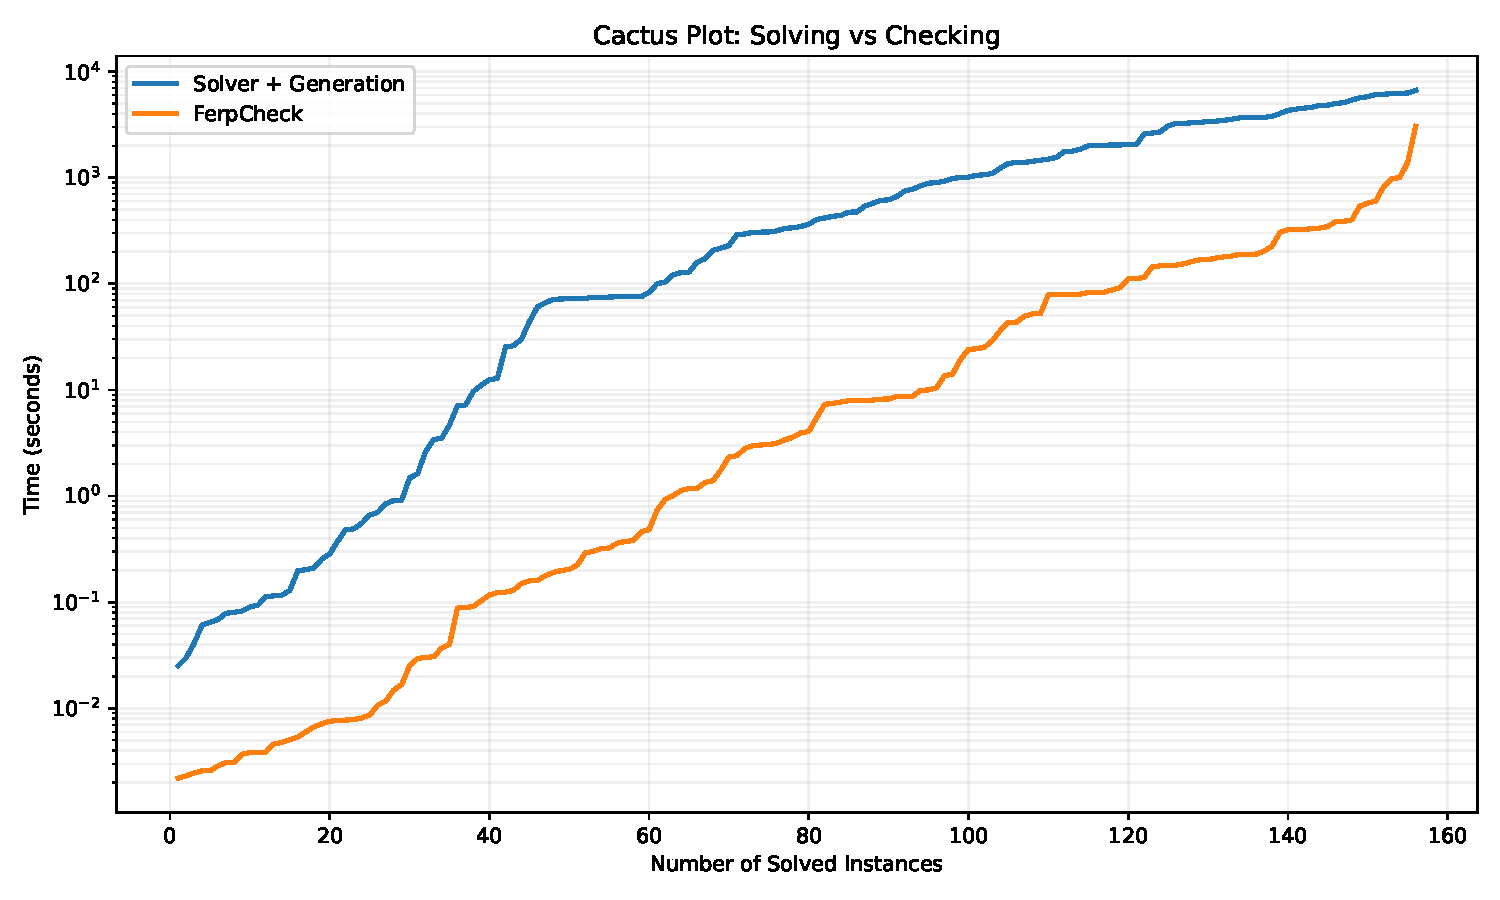
\includegraphics[width=\textwidth, keepaspectratio]{solving_vs_checking.pdf}
        %\caption{First description} % Optional
    \end{minipage}
    \hfill % Adds horizontal space between the two images
    \begin{minipage}{0.4\textwidth}
        \centering
        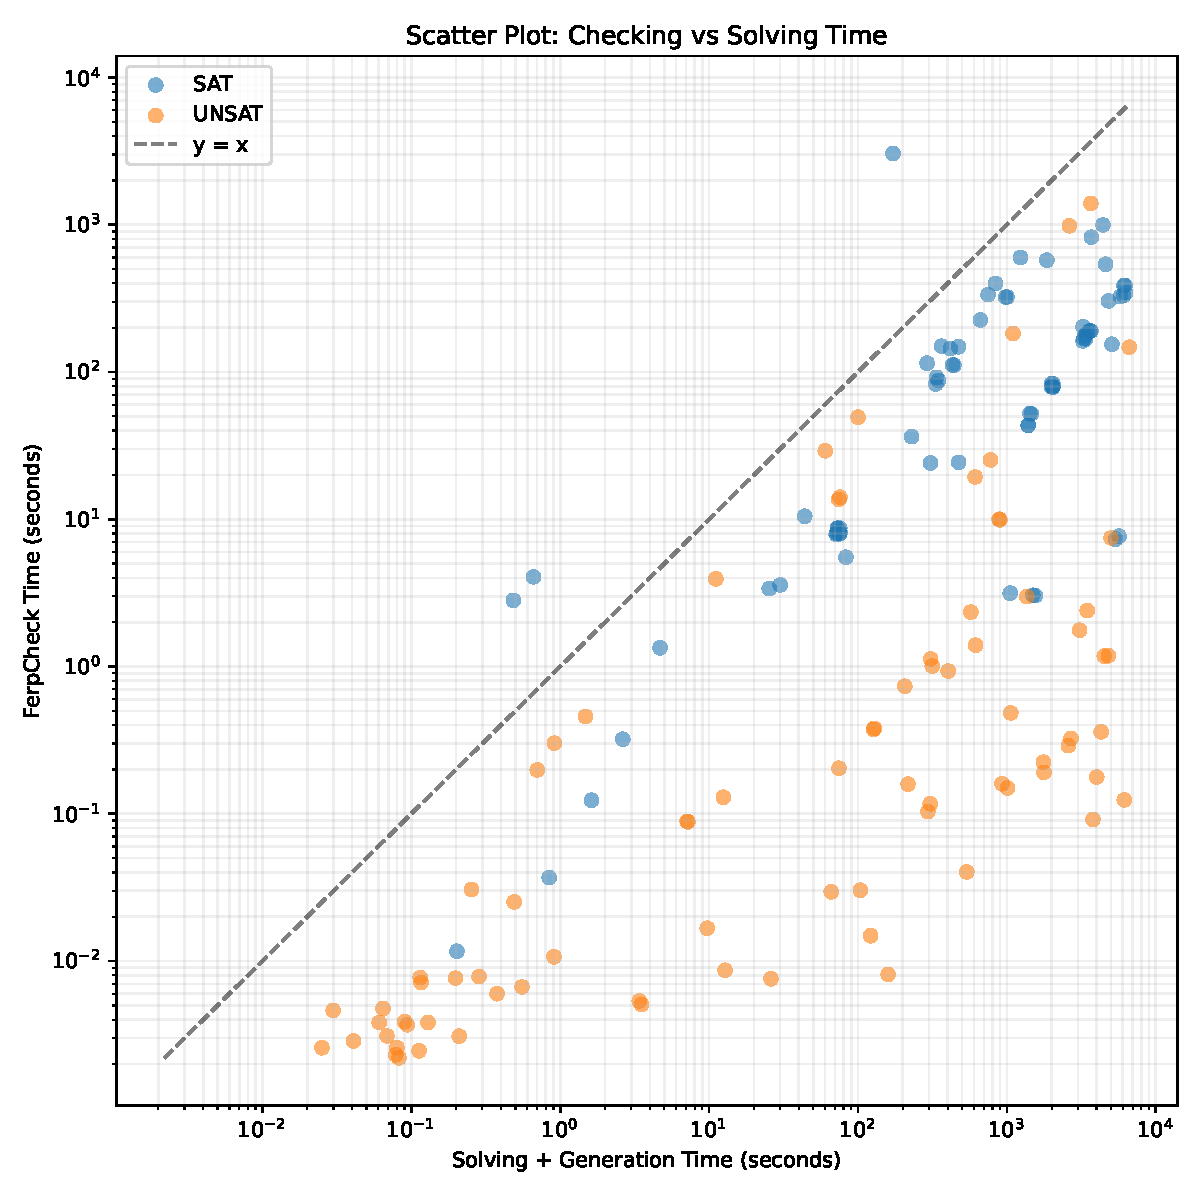
\includegraphics[width=\textwidth, keepaspectratio]{scat_solving_vs_checking.pdf}
        %\caption{Second description} % Optional
    \end{minipage}
\end{frame}

\begin{frame}{Future Work}

    \begin{itemize}
        \setlength{\itemsep}{12pt}
              \only<1->{\item Proof trimming for $\exists$-expansion proofs.}
              \only<2->{\item Skolem function extraction from verified $\exists$-expansion proofs.}
              \only<3->{\item Extensive experiments comparing to other proof system implementations (QBFCert, FERAT, FERPModels, CAQE, etc.).}
    \end{itemize}

\end{frame}


\contactframe[light]{%
    Sidhant Bhavnani
}{%
    Institute of Symbolic Artificial Intelligence
}{%
    \contactmail{sidhant.bhavnani@jku.at}
    \contactweb[https://s1db.github.io]{s1db.github.io}
}{%
    This research was funded in whole or in part by the Austrian Science Fund (FWF) 10.55776/COE12. For open access purposes, the author has applied a CC BY public copyright license.
}


\begin{comment}

    \begin{frame}{Introduction \& The Core Asymmetry}
        \small

        % Section 1: Unified Checking Pipeline (Visual TikZ Flow)
        \begin{block}{The Complete Checking \& Verification Pipeline}
            \centering
            \vspace{0.15cm}
            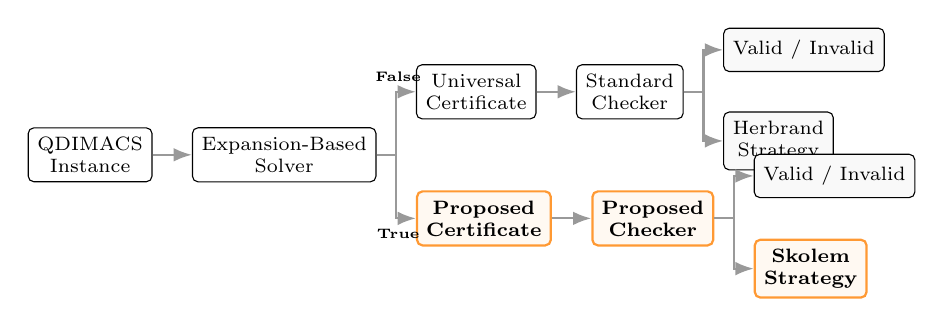
\begin{tikzpicture}[
                    node distance=0.15cm and 0.5cm,
                    block/.style={draw, rectangle, rounded corners=2pt, minimum height=0.55cm, align=center, font=\scriptsize, fill=white, thin},
                    contrib/.style={draw=orange!80, thick, rectangle, rounded corners=2pt, minimum height=0.55cm, align=center, font=\scriptsize\bfseries, fill=orange!5},
                    arrow/.style={-Latex, thick, draw=gray!80}
                ]
                % Input & Solver
                \node[block] (input) {QDIMACS\\Instance};
                \node[block, right=of input] (solver) {Expansion-Based\\Solver};

                % False branch (Top Baseline)
                \node[block, above right=0.1cm and 0.5cm of solver] (cert_f) {Universal\\Certificate};
                \node[block, right=of cert_f] (checker_f) {Standard\\Checker};
                \node[block, above right=-0.1cm and 0.5cm of checker_f, fill=gray!5] (verdict_f) {Valid / Invalid};
                \node[block, below right=-0.1cm and 0.5cm of checker_f, fill=gray!5] (strat_f) {Herbrand\\Strategy};

                % True branch (Bottom Contribution)
                \node[contrib, below right=0.1cm and 0.5cm of solver] (cert_t) {Proposed\\Certificate};
                \node[contrib, right=of cert_t] (checker_t) {Proposed\\Checker};
                \node[block, above right=-0.1cm and 0.5cm of checker_t, fill=gray!5] (verdict_t) {Valid / Invalid};
                \node[contrib, below right=-0.1cm and 0.5cm of checker_t] (strat_t) {Skolem\\Strategy};

                % Connections
                \draw[arrow] (input) -- (solver);
                \draw[arrow] (solver.east) -- ++(0.25,0) |- node[above, pos=0.55, font=\tiny\bfseries] {False} (cert_f.west);
                \draw[arrow] (solver.east) -- ++(0.25,0) |- node[below, pos=0.55, font=\tiny\bfseries] {True} (cert_t.west);
                \draw[arrow] (cert_f) -- (checker_f);
                \draw[arrow] (cert_t) -- (checker_t);

                \draw[arrow] (checker_f.east) -- ++(0.25,0) |- (verdict_f.west);
                \draw[arrow] (checker_f.east) -- ++(0.25,0) |- (strat_f.west);
                \draw[arrow] (checker_t.east) -- ++(0.25,0) |- (verdict_t.west);
                \draw[arrow] (checker_t.east) -- ++(0.25,0) |- (strat_t.west);
            \end{tikzpicture}
            \vspace{0.15cm}
        \end{block}

        \vspace{0.1cm}

        % Section 2: Divergence Table
        \begin{block}{Axiom Definitions \& Algorithmic Divergence}
            \centering
            \scriptsize
            \renewcommand{\arraystretch}{1.2}
            \begin{tabular}{l p{4.5cm} p{4.5cm}}
                \toprule
                \textbf{Metric}              & \textbf{Universal Expansion ($\forall$-Exp)}          & \textbf{Existential Expansion ($\exists$-Exp)}      \\
                \midrule
                \textbf{Axiom Definition}    & $\psi_\forall = \bigwedge_{\alpha \in A} \phi^\alpha$ & $\psi_\exists = \bigvee_{\sigma \in S} \phi^\sigma$ \\
                \textbf{Structure (Negated)} & Natively clausal (CNF)                                & Non-clausal (Conjunction of DNFs)                   \\
                \textbf{SAT Target}          & Satisfiability Check ($\psi_\forall = \bot$)          & Validity Check ($\neg \psi_\exists = \bot$)         \\
                \textbf{Verification Status} & Automated tools available (\texttt{FERAT})            & No algorithm available (prior to this work)         \\
                \bottomrule
            \end{tabular}
        \end{block}
    \end{frame}


    \begin{frame}{Introduction \& The Core Asymmetry}
        \small

        % % Section 1: Macro-Context
        % \begin{alertblock}{The Engineering ``Why''}
        %     \footnotesize
        %     Expansion-based solvers reduce the QBF decision problem to propositional satisfiability by evaluating partial expansions over blocks of quantifiers. However, the logical structure generated by this paradigm diverges completely depending on whether the instance is true or false.
        % \end{alertblock}

        \vspace{0.1cm}

        % Section 2: Complete Checking Pipelines
        \begin{block}{The Complete Checking Pipelines}
            \scriptsize
            \begin{tabular}{r c l}
                \textbf{False Instance:}           & $\Phi^\bot \longrightarrow \psi_\forall \text{ (Universal Expansion)} \longrightarrow \text{Pure CNF} \longrightarrow \text{SAT} \longrightarrow \forall\text{Exp+Res Proof} \longrightarrow \text{Standard Checker}$                  \\[4pt]
                \textbf{True Instance (Proposed):} & $\Phi^\top \longrightarrow \psi_\exists \text{ (Existential Expansion)} \longrightarrow \text{Disjunction of CNFs} \longrightarrow \text{Negation + PG} \longrightarrow \text{Equisatisfiable CNF} \longrightarrow \text{Our Checker}$
            \end{tabular}
        \end{block}

        \vspace{0.1cm}

        % Section 3: Divergence Table
        \begin{block}{Axiom Definitions \& Algorithmic Divergence}
            \centering
            \scriptsize
            \renewcommand{\arraystretch}{1.1}
            \begin{tabular}{l p{5cm} p{5.5cm}}
                \toprule
                \textbf{Metric}              & \textbf{Universal Expansion ($\forall$-Exp)}                                & \textbf{Existential Expansion ($\exists$-Exp)}                \\
                \midrule
                \textbf{Axiom Definition}    & $\psi_\forall = \bigwedge_{\alpha \in A} \phi^\alpha$                       & $\psi_\exists = \bigvee_{\sigma \in S} \phi^\sigma$           \\
                \textbf{Clausal Structure}   & \textbf{Stays in CNF} (Natively clausal)                                    & \textbf{Not in CNF} (Conjunction of DNFs under negation)      \\
                \textbf{Target SAT Check}    & Satisfiability Check ($\psi_\forall = \bot$)                                & Validity Check via Negation ($\neg \psi_\exists = \bot$)      \\
                \textbf{Verification Status} & \textbf{Checking algorithm available} (\texttt{FERAT}, \texttt{FERPModels}) & \textbf{No checking algorithm available} (prior to this work) \\
                \bottomrule
            \end{tabular}
        \end{block}
    \end{frame}


    \begin{frame}{Introduction}
        \centering
        \scriptsize

        \vspace{-3cm}

        \[
            \forall x.\,\phi \equiv \phi[x/0] \wedge \phi[x/1]
            \qquad\qquad
            \exists x.\,\phi \equiv \phi[x/0] \vee \phi[x/1]
        \]
        \[
            \text{\tiny CNF --- SAT check}
            \qquad\qquad\qquad\qquad\quad
            \text{\tiny non-CNF --- validity check}
        \]

        \vspace{0.1cm}

        \begin{tikzpicture}[
                box/.style={draw, rounded corners=2pt, inner sep=4pt,
                        font=\tiny, align=center, minimum width=1.6cm},
                dia/.style={draw, diamond, inner sep=2pt,
                        font=\tiny, align=center},
                arr/.style={->, thin},
                larr/.style={->, thin, blue!70!black},
                rarr/.style={->, thin, orange!70!black}
            ]

            %--- Left loop: universal expansion ---
            \node[box] (forall) at (-2.8, 0)    {$\forall$-Expansion};
            \node[dia] (sat)    at (-2.8, -1.2) {SAT?};
            \node[box] (false)  at (-2.8, -2.4) {QBF False};
            \node[box] (certL)  at (-2.8, -3.4) {Certificate};

            \draw[larr] (forall) -- (sat);
            \draw[larr] (sat)    -- node[right, font=\tiny] {YES} (false);
            \draw[larr] (false)  -- (certL);

            %--- Right loop: existential expansion ---
            \node[box] (exists) at (2.8, 0)    {$\exists$-Expansion};
            \node[dia] (valid)  at (2.8, -1.2) {VALID?};
            \node[box] (true)   at (2.8, -2.4) {QBF True};
            \node[box] (certR)  at (2.8, -3.4) {Certificate};

            \draw[rarr] (exists) -- (valid);
            \draw[rarr] (valid)  -- node[right, font=\tiny] {YES} (true);
            \draw[rarr] (true)   -- (certR);

            %--- Cross connections through center ---
            \draw[arr] (sat.east)   -- node[above, font=\tiny] {NO}
            ($(sat.east)!0.5!(valid.west)$) |- (exists.west);
            \draw[arr] (valid.west) -- node[above, font=\tiny] {NO}
            ($(valid.west)!0.5!(sat.east)$) |- (forall.east);

            %--- Checker box ---
            \node[box, minimum width=2.0cm] (checker) at (0, -4.6) {Checker};

            \draw[larr] (certL.south) |- (checker.west);
            \draw[rarr] (certR.south) |- (checker.east);

            %--- Checker outputs ---
            \draw[arr] (checker.south) -- ++(0, -0.4)
            node[below, font=\tiny] {Valid / Invalid certificate};
            \draw[arr] (checker.south) -- ++(0, -0.4) -- ++(1.2, 0)
            node[right, font=\tiny] {Strategy};

        \end{tikzpicture}

        \vspace{0.15cm}
        \textbf{No proof format or checking algorithm exists for the true case --- this talk presents both.}

    \end{frame}



    \begin{frame}{Universal Expansion}
        \footnotesize
        $$\forall x.\, \phi \;\equiv\; \textcolor{blue}{\phi[x/0]} \wedge \textcolor{red}{\phi[x/1]}$$
        \begin{flalign*}
             & \Pi_1\, \forall u\, \Pi_2.\, \phi                                                                                                                       &   & \\[4pt]
             & \only<2>{\Pi_1\, \Bigl(\textcolor{blue}{\Pi_2}.\, \textcolor{blue}{\phi[u/0]} \;\wedge\; \textcolor{red}{\Pi_2}.\, \textcolor{red}{\phi[u/1]}\Bigr)}          %
            \only<3>{\Pi_1\, \Bigl(\textcolor{blue}{\Pi_2^{u/0}}.\, \textcolor{blue}{\phi[u/0]} \;\wedge\; \textcolor{red}{\Pi_2^{u/1}}.\, \textcolor{red}{\phi[u/1]}\Bigr)}%
            \only<4->{\Pi_1\, \Bigl(\textcolor{blue}{\Pi_2^{\bar u}}.\, \textcolor{blue}{\phi^{\bar u}} \;\wedge\; \textcolor{red}{\Pi_2^{u}}.\, \textcolor{red}{\phi^{u}}\Bigr)}%
             &                                                                                                                                                         &     \\[4pt]
             & \onslide<5->{\Pi_1\, \textcolor{blue}{\Pi_2^{\bar u}}\, \textcolor{red}{\Pi_2^{u}}.\; \textcolor{blue}{\phi^{\bar u}} \wedge \textcolor{red}{\phi^{u}}} &   &
        \end{flalign*}
    \end{frame}

    \begin{frame}{Universal Expansion (Example)}
        \footnotesize
        \[
            \forall a_1\, \exists e_2\, \forall a_3\, \exists e_5.\quad
            (a_1 \vee a_3 \vee e_2) \wedge (a_1 \vee \neg a_3 \vee \neg e_2) \wedge (\neg a_1 \vee e_5) \wedge (\neg a_1 \vee \neg e_5)
        \]

        \onslide<2->{is equivalent to}

        %--- Step 2: expand a3 ---
        \only<2>{
                \[
                    \forall a_1\, \exists e_2\, e_5^{\overline{a}_3}\, e_5^{a_3}.
                \]
                \[
                    \underbrace{(a_1 \vee 0 \vee e_2) \wedge (a_1 \vee 1 \vee \neg e_2) \wedge (\neg a_1 \vee e_5^{\overline{a}_3}) \wedge (\neg a_1 \vee \neg e_5^{\overline{a}_3})}_{\phi[a_3/0]} \;\wedge
                \]
                \[
                    \underbrace{(a_1 \vee 1 \vee e_2) \wedge (a_1 \vee 0 \vee \neg e_2) \wedge (\neg a_1 \vee e_5^{a_3}) \wedge (\neg a_1 \vee \neg e_5^{a_3})}_{\phi[a_3/1]}
                \]
            }

        %--- Step 3: expand a1 as well (full expansion) ---
        \only<3>{
                \[
                    \exists\, e_2^{\overline{a}_1}\, e_2^{a_1}\, e_5^{\overline{a}_1,\overline{a}_3}\, e_5^{\overline{a}_1,a_3}\, e_5^{a_1,\overline{a}_3}\, e_5^{a_1,a_3}.
                \]
                \[
                    (0 \vee 0 \vee e_2^{\overline{a}_1}) \wedge (0 \vee 1 \vee \neg e_2^{\overline{a}_1}) \wedge (1 \vee e_5^{\overline{a}_1, \overline{a}_3}) \wedge (1 \vee \neg e_5^{\overline{a}_1, \overline{a}_3}) \;\wedge
                \]
                \[
                    (0 \vee 1 \vee e_2^{\overline{a}_1}) \wedge (0 \vee 0 \vee \neg e_2^{\overline{a}_1}) \wedge (1 \vee e_5^{\overline{a}_1, a_3}) \wedge (1 \vee \neg e_5^{\overline{a}_1, a_3}) \;\wedge
                \]
                \[
                    (1 \vee 0 \vee e_2^{a_1}) \wedge (1 \vee 1 \vee \neg e_2^{a_1}) \wedge (0 \vee e_5^{a_1, \overline{a}_3}) \wedge (0 \vee \neg e_5^{a_1, \overline{a}_3}) \;\wedge
                \]
                \[
                    (1 \vee 1 \vee e_2^{a_1}) \wedge (1 \vee 0 \vee \neg e_2^{a_1}) \wedge (0 \vee e_5^{a_1, a_3}) \wedge (0 \vee \neg e_5^{a_1, a_3})
                \]
            }

        %--- Step 4: remove satisfied clauses ---
        \only<4>{
                \[
                    \exists\, e_2^{\overline{a}_1}\, e_5^{a_1,\overline{a}_3}\, e_5^{a_1,a_3}.
                \]
                \[
                    (0 \vee 0 \vee e_2^{\overline{a}_1}) \;\wedge\; (0 \vee 0 \vee \neg e_2^{\overline{a}_1}) \;\wedge\; (0 \vee e_5^{a_1, \overline{a}_3}) \;\wedge\; (0 \vee \neg e_5^{a_1, \overline{a}_3}) \;\wedge\; (0 \vee e_5^{a_1, a_3}) \;\wedge\; (0 \vee \neg e_5^{a_1, a_3})
                \]
            }

        %--- Step 5: remove 0 literals, one line ---
        \only<5>{
                \[
                    \exists\, e_2^{\overline{a}_1}\, e_5^{a_1,\overline{a}_3}\, e_5^{a_1,a_3}.
                \]
                \[
                    (e_2^{\overline{a}_1}) \wedge (\neg e_2^{\overline{a}_1}) \wedge (e_5^{a_1, \overline{a}_3}) \wedge (\neg e_5^{a_1, \overline{a}_3}) \wedge (e_5^{a_1, a_3}) \wedge (\neg e_5^{a_1, a_3})
                \]
            }

        % %--- Step 6: A, falsity ---
        % \only<6->{
        % \[
        %     \exists\, e_2^{\overline{a}_1}\, e_5^{a_1,\overline{a}_3}\, e_5^{a_1,a_3}.
        % \]
        % \[
        %     (e_2^{\overline{a}_1}) \wedge (\neg e_2^{\overline{a}_1}) \wedge (e_5^{a_1, \overline{a}_3}) \wedge (\neg e_5^{a_1, \overline{a}_3}) \wedge (e_5^{a_1, a_3}) \wedge (\neg e_5^{a_1, a_3})
        % \]
        % \medskip
        % \[
        %     \psi_\forall = \phi^{\overline{a}_1\overline{a}_3} \wedge \phi^{\overline{a}_1 a_3} = (e_2^{\overline{a}_1}) \wedge (\neg e_2^{\overline{a}_1}) = \bot
        %     \qquad A = \{\overline{a}_1\overline{a}_3,\ \overline{a}_1 a_3\}
        % \]
        % }

        % %--- Step 7: A' appears below ---
        % \only<7->{
        % \[
        %     \psi_\forall' = \phi^{a_1\overline{a}_3} \wedge \phi^{a_1 a_3} = (e_5^{a_1,\overline{a}_3}) \wedge (\neg e_5^{a_1,\overline{a}_3}) \wedge (e_5^{a_1,a_3}) \wedge (\neg e_5^{a_1,a_3}) = \bot
        %     \qquad A' = \{a_1\overline{a}_3,\ a_1 a_3\}
        % \]
        % }

    \end{frame}


    \begin{frame}{Expansion by Assignments to Universals}

        \small

        A \emph{universal assignment} $\alpha : U_\Pi \to \mathbb{B}$ instantiates all universal variables at once, yielding an instantiation $\phi^\alpha$.

        \medskip
        A \emph{partial universal expansion} over a finite set $A$ of universal assignments is
        \[
            \psi_\forall = \bigwedge_{\alpha \in A} \phi^\alpha
        \]

        Since $\phi$ is in CNF, so is each $\phi^\alpha$, and hence so is $\psi_\forall$ --- it passes directly to a SAT solver.

        \medskip
        $\Phi$ is false if and only if there exists a finite $A$ such that $\psi_\forall$ is unsatisfiable.

    \end{frame}





    \begin{frame}{}
        \small
        \[
            \Phi^\bot \;=\; \exists e_1\;\forall u_2\;\exists e_3.\quad
            \underbrace{(e_1 \vee u_2 \vee e_3)}_{C_1} \wedge
            \underbrace{(\neg e_1 \vee \neg u_2 \vee e_3)}_{C_2} \wedge
            \underbrace{(\neg e_3)}_{C_3}
        \]

        \begin{center}
            \begin{tikzpicture}[
                    qbf/.style={draw, rounded corners=2pt, inner sep=4pt, font=\scriptsize},
                    sat/.style={draw, fill=white, rounded corners=2pt, inner sep=4pt, font=\scriptsize},
                    res/.style={draw, rounded corners=2pt, inner sep=4pt, font=\scriptsize},
                    ea/.style={->, thick, blue!70!black},
                    ra/.style={->, thick, orange!70!black},
                    hlbox/.style={draw=red!70!black, thin, dotted, rounded corners=2pt, inner sep=2pt}
                ]

                % QBF clause nodes
                \node[qbf] (C1) at (0.5,  0)   {$(e_1 \vee u_2 \vee e_3)$};
                \node[qbf] (C2) at (3.5,  0)   {$(\neg e_1 \vee \neg u_2 \vee e_3)$};
                \node[qbf] (C3) at (6.5,  0)   {$(\neg e_3)$};

                % SAT clause nodes
                \node[sat] (S1) at (0.0, -1.5) {$e_1 \vee e_3^{u\leftarrow \bot}$};
                \node[sat] (S2) at (2.8, -1.5) {$\neg e_1 \vee e_3^{u\leftarrow \top}$};
                \node[sat] (S3) at (5.2, -1.5) {$\neg e_3^{u\leftarrow \bot}$};
                \node[sat] (S4) at (7.6, -1.5) {$\neg e_3^{u\leftarrow \top}$};

                % Expansion arrows
                \draw[ea] (C1) -- (S1);
                \draw[ea] (C2) -- (S2);
                \draw[ea] (C3) -- (S3);
                \draw[ea] (C3) -- (S4);

                % Refutation nodes
                \node[res] (R1) at (1.5, -3) {$e_3^{u\leftarrow \bot} \vee e_2^{u\leftarrow \top}$};
                \node[res] (R2) at (4.5, -4) {$e_3^{u\leftarrow \top}$};
                \node[res] (BOT) at (6.0, -5.2) {$\bot$};

                % Refutation arrows
                \draw[ra] (S1) -- (R1);
                \draw[ra] (S2) -- (R1);
                \draw[ra] (S3) -- (R2);
                \draw[ra] (R1) -- (R2);
                \draw[ra] (R2) -- (BOT);
                \draw[ra] (S4) -- (BOT);

                % Legend
                \node[font=\footnotesize] at (1.5, -6.2)
                {\textcolor{blue!70!black}{$\longrightarrow$ expansion}};
                \node[font=\footnotesize] at (5.5, -6.2)
                {\textcolor{orange!70!black}{$\longrightarrow$ resolution}};

                % Step 2: highlight u=0 clauses + arrows
                \only<2>{
                        \node[hlbox, fit=(C1)(S1)] {};
                        \node[hlbox, fit=(C3)(S3)] {};
                        \draw[thick, dotted, red!70!black, ->] (C1) -- (S1);
                        \draw[thick, dotted, red!70!black, ->] (C3) -- (S3);
                    }

                % Step 3: highlight u=1 clauses + arrows
                \only<3>{
                        \node[hlbox, fit=(C2)(S2)] {};
                        \node[hlbox, fit=(C3)(S4)] {};
                        \draw[thick, dotted, red!70!black, ->] (C2) -- (S2);
                        \draw[thick, dotted, red!70!black, ->] (C3) -- (S4);
                    }

                % Step 4: divider line through axiom clauses, behind them
                \only<4->{
                        \begin{pgfonlayer}{background}
                            \draw[dotted, thick] (-3, -1.5) -- (8.8, -1.5);
                        \end{pgfonlayer}

                        \node[font=\footnotesize, align=center] at (-2.0, -0.8) {$\forall$-expansion};
                        \node[font=\footnotesize, align=center] at (-2.0, -2.2) {resolution};
                    }

            \end{tikzpicture}
        \end{center}
    \end{frame}


    \begin{frame}{Certifying the False Case}
        \small

        \begin{columns}[T]
            \begin{column}{0.35\textwidth}
                \\[2pt]\textbf{Proof}\\[4pt]
                \small
                \only<2->{\texttt{x\ \ 1\ 0\ 1\ 0\ \ \ \ 0}}\strut\\
                \only<2->{\texttt{x\ \ 2\ 0\ 3\ 0\ -2\ 0}}\strut\\
                \only<3->{\texttt{x\ \ 3\ 0\ 3\ 0\ \ 2\ 0}}\strut\\
                \smallskip
                \only<2->{\texttt{a\ \ 1\ \ 2\ 0\ 1}}\strut\\
                \only<2->{\texttt{a\ -2\ \ \ \ 0\ 3}}\strut\\
                \only<3->{\texttt{a\ -1\ \ 3\ 0\ 2}}\strut\\
                \only<3->{\texttt{a\ -3\ \ \ \ 0\ 3}}\strut\\
                \smallskip
                \only<4->{\texttt{r\ \ 2\ 3\ 0}}\strut\\
                \only<5->{\texttt{r\ \ 3\ \ 0}}\strut\\
                \only<6->{\texttt{r\ \ 0}}
            \end{column}

            \begin{column}{0.58\textwidth}
                \begin{center}
                    \scalebox{0.8}{%
                        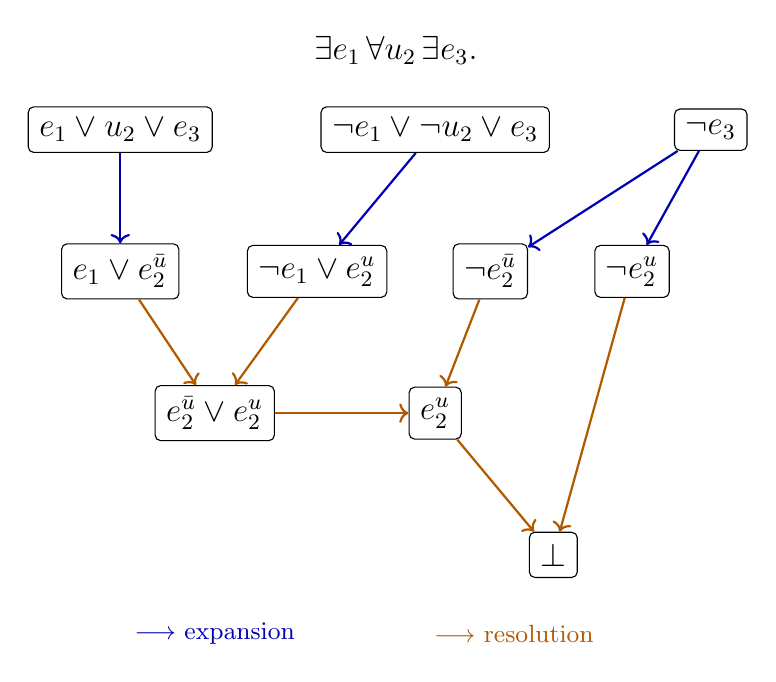
\begin{tikzpicture}[
                                qbf/.style={draw, rounded corners=2pt, inner sep=4pt, font=\large},
                                sat/.style={draw, rounded corners=2pt, inner sep=4pt, font=\large},
                                res/.style={draw, rounded corners=2pt, inner sep=4pt, font=\large},
                                ea/.style={->, thick, blue!70!black},
                                ra/.style={->, thick, orange!70!black}
                            ]

                            % Quantifier prefix
                            \node[font=\large] at (3.5, 1.0) {$\exists e_1\, \forall u_2\, \exists e_3.$};

                            % QBF clauses
                            \node[qbf] (C1) at (0, 0)   {$e_1 \vee u_2 \vee e_3$};
                            \node[qbf] (C2) at (4, 0)   {$\neg e_1 \vee \neg u_2 \vee e_3$};
                            \node[qbf] (C3) at (7.5, 0) {$\neg e_3$};

                            % Axiom clauses
                            \node[sat, visible on=<2->] (S1) at (0, -1.8)   {$e_1 \vee e_2^{\bar u}$};
                            \node[sat, visible on=<3->] (S2) at (2.5, -1.8) {$\neg e_1 \vee e_2^{u}$};
                            \node[sat, visible on=<2->] (S3) at (4.7, -1.8) {$\neg e_2^{\bar u}$};
                            \node[sat, visible on=<3->] (S4) at (6.5, -1.8) {$\neg e_2^{u}$};

                            % Expansion arrows
                            \draw[ea, visible on=<2->] (C1) -- (S1);
                            \draw[ea, visible on=<2->] (C3) -- (S3);
                            \draw[ea, visible on=<3->] (C2) -- (S2);
                            \draw[ea, visible on=<3->] (C3) -- (S4);

                            % Refutation nodes
                            \node[res, visible on=<4->] (R1) at (1.2, -3.6) {$e_2^{\bar u} \vee e_2^{u}$};
                            \node[res, visible on=<5->] (R2) at (4.0, -3.6) {$e_2^{u}$};
                            \node[res, visible on=<6->] (BOT) at (5.5, -5.4) {$\bot$};

                            % Refutation arrows
                            \draw[ra, visible on=<4->] (S1) -- (R1);
                            \draw[ra, visible on=<4->] (S2) -- (R1);
                            \draw[ra, visible on=<5->] (S3) -- (R2);
                            \draw[ra, visible on=<5->] (R1) -- (R2);
                            \draw[ra, visible on=<6->] (R2) -- (BOT);
                            \draw[ra, visible on=<6->] (S4) -- (BOT);

                            % Legend
                            \node[font=\small] at (1.2, -6.4)
                            {\textcolor{blue!70!black}{$\longrightarrow$ expansion}};
                            \node[font=\small] at (5.0, -6.4)
                            {\textcolor{orange!70!black}{$\longrightarrow$ resolution}};

                        \end{tikzpicture}}
                \end{center}
            \end{column}
        \end{columns}

    \end{frame}

    \begin{frame}{Checking Expansions}
        \small
        \vspace{-0.8cm}
        \[
            \exists e_1\, \forall u_2\, \exists e_3.\quad
            \underbrace{(e_1 \vee u_2 \vee e_3)}_{C_1} \wedge
            \underbrace{(\neg e_1 \vee \neg u_2 \vee e_3)}_{C_2} \wedge
            \underbrace{(\neg e_3)}_{C_3}
        \]
        \begin{columns}[T]
            \begin{column}{0.25\textwidth}
                \vspace{-0.8cm}
                \hspace{0.4cm}
                \\[2pt]\textbf{Proof}\\[4pt]
                \small
                \texttt{x\ \ }\alt<4>{\textcolor{red}{\textbf{\texttt{1 \textcolor{black}{0} 1}}}}{\texttt{1 0 1}}\texttt{ 0\ \ \ \ 0}\strut\\
                \texttt{x\ \ }\alt<4>{\textcolor{red}{\textbf{\texttt{2 \textcolor{black}{0} 3}}}}{\texttt{2 0 3}}\texttt{ 0 }\alt<5>{\textcolor{red}{\textbf{\texttt{-2}}}}{\texttt{-2}}\texttt{ 0}\strut\\
                \texttt{x\ \ 3\ 0\ 3\ 0\ \ 2\ 0}\strut\\
                \smallskip
                \alt<2>{{\setlength{\fboxsep}{0pt}\colorbox{yellow!50}{\texttt{a\ \ 1\ \ 2\ 0\ 1}}}}{\alt<3>{\texttt{a\ \ 1\ \ 2\ 0\ }\textcolor{red}{\textbf{\texttt{1}}}}{\texttt{a\ \ 1\ \ 2\ 0\ 1}}}\strut\\
                \texttt{a\ -2\ \ \ \ 0\ 3}\strut\\
                \texttt{a\ -1\ \ 3\ 0\ 2}\strut\\
                \texttt{a\ -3\ \ \ \ 0\ 3}
            \end{column}
            \begin{column}{0.7\textwidth}
                \scriptsize
                \textbf{\alt<1>{For each axiom clause $D$ in the proof, check:}{Checking $D = (e_1 \vee e_2^{\bar u})$:}}\\[4pt]
                \hspace{0.5cm} \alt<3>{\textcolor{red}{\textbf{1.\ Retrieve origin clause $C$}}}{1.\ Retrieve origin clause $C$}\\[1pt]
                \hspace{0.5cm} \alt<4>{\textcolor{red}{\textbf{2.\ Check $D$ and $C$ contain the same existentials (after undoing annotations)}}}{2.\ Check $D$ and $C$ contain the same existentials (after undoing annotations)}\\[1pt]
                \hspace{0.5cm} \alt<5>{\textcolor{red}{\textbf{3.\ Read the universal assignment off $D$'s annotations}}}{3.\ Read the universal assignment off $D$'s annotations}\\[1pt]
                \hspace{0.5cm} \alt<6>{\textcolor{red}{\textbf{4.\ Check this assignment falsifies every universal literal of $C$}}}{4.\ Check this assignment falsifies every universal literal of $C$}

                \vspace{-2pt}
                \begin{align*}
                    \onslide<3->{C &= C_1 = (e_1 \vee u \vee e_2)}                               \\
                    \onslide<4->{\text{ex.}(C) &= \{e_1, e_2\} \;=\; \text{ex.}(D) \;\checkmark} \\
                    \onslide<5->{\text{assignment} &= \bar u}                                    \\
                    \onslide<6->{\text{univ.}(C) &= u \;\;\text{falsified by } \bar u \;\checkmark}
                \end{align*}
            \end{column}
        \end{columns}
    \end{frame}

    \section{Existential Expansion and True QBFs}


    \iffalse
        \begin{frame}{Existential Expansion}
            \footnotesize
            $$\exists x.\, \phi \;\equiv\; \textcolor{blue}{\phi[x/0]} \vee \textcolor{red}{\phi[x/1]}$$
            \begin{flalign*}
                 & \Pi_1\, \exists u\, \Pi_2.\, \phi                                                                                                                     &   & \\[4pt]
                 & \only<2>{\Pi_1\, \Bigl(\textcolor{blue}{\Pi_2}.\, \textcolor{blue}{\phi[u/0]} \;\vee\; \textcolor{red}{\Pi_2}.\, \textcolor{red}{\phi[u/1]}\Bigr)}          %
                \only<3>{\Pi_1\, \Bigl(\textcolor{blue}{\Pi_2^{u/0}}.\, \textcolor{blue}{\phi[u/0]} \;\vee\; \textcolor{red}{\Pi_2^{u/1}}.\, \textcolor{red}{\phi[u/1]}\Bigr)}%
                \only<4->{\Pi_1\, \Bigl(\textcolor{blue}{\Pi_2^{\bar u}}.\, \textcolor{blue}{\phi^{\bar u}} \;\vee\; \textcolor{red}{\Pi_2^{u}}.\, \textcolor{red}{\phi^{u}}\Bigr)}%
                 &                                                                                                                                                       &     \\[4pt]
                 & \onslide<5->{\Pi_1\, \textcolor{blue}{\Pi_2^{\bar u}}\, \textcolor{red}{\Pi_2^{u}}.\; \textcolor{blue}{\phi^{\bar u}} \vee \textcolor{red}{\phi^{u}}} &   &
            \end{flalign*}
        \end{frame}



        \begin{frame}{Existential Expansion (Example)}
            \footnotesize

            \[
                \forall a\, \exists e\, \forall b.\quad
                (e \vee a \vee b) \wedge (\neg e \vee \neg a \vee \neg b) \wedge (\neg e \vee \neg a \vee b)
            \]

            is equivalent to

            \[
                \forall a b^{\bar e}\, b^{e}.
            \]
            \[
                \underbrace{\bigl[(0 \vee a \vee b^{\bar e}) \wedge (\neg 0 \vee \neg a \vee \neg b^{\bar e}) \wedge (\neg 0 \vee \neg a \vee b^{\bar e})\bigr]}_{\phi[e/0]}
                \;\vee\;
                \underbrace{\bigl[(1 \vee a \vee b^{e}) \wedge (\neg 1 \vee \neg a \vee \neg b^{e}) \wedge (\neg 1 \vee \neg a \vee b^{e})\bigr]}_{\phi[e/1]}
            \]

            \onslide<2->{
                    simplifies to
                    \[
                        \forall a b^{\bar e}\, b^{e}.\quad
                        \underbrace{(a \vee b^{\bar e})}_{\phi^{\bar e}}
                        \;\vee\;
                        \underbrace{(\neg a \vee \neg b^{e}) \wedge (\neg a \vee b^{e})}_{\phi^{e}}
                    \]
                }
        \end{frame}


        \begin{frame}{Validity via Negation}
            \footnotesize

            $\Phi$ is true iff $\psi_\exists = \bigvee_{\sigma\in S} \phi^\sigma$ is valid:
            \[
                \forall\; \bigvee_{\sigma \in S}\phi^\sigma = \top
                \quad\Longleftrightarrow\quad
                \bigwedge_{\sigma \in S}\neg\phi^\sigma = \bot
            \]

            \medskip
            \textbf{Negating the example:}
            \[
                \neg\psi_\exists \;=\;
                \underbrace{(\neg a \wedge \neg b^{\bar e})}_{\neg\phi^{\bar e}\;\text{(DNF)}}
                \;\wedge\;
                \underbrace{\bigl[(a \wedge b^{e}) \vee (a \wedge \neg b^{e})\bigr]}_{\neg\phi^{e}\;\text{(DNF)}}
            \]

            Each $\neg\phi^\sigma$ is in DNF --- not directly passable to a SAT solver.
        \end{frame}












        \begin{frame}{Existential Expansion}

            \tiny

            \textbf{Rule:}
            \[
                \exists x.\; \phi \;=\; \phi[x/0] \vee \phi[x/1]
            \]

            % \medskip
            \textbf{Example:}
            \[
                \Phi^\top \;=\; \forall a\; \exists e\; \forall b.\;
                (e \vee a \vee b) \wedge
                (\neg e \vee \neg a \vee \neg b) \wedge
                (\neg e \vee \neg a \vee b)
            \]

            Expanding $e$; universal variable $b$ becomes annotated copies $b^{e\leftarrow \bot}$, $b^{e\leftarrow \top}$:
            \[
                \psi_\exists \;=\;
                \underbrace{\bigl[(\neg a \vee \neg b^{e\leftarrow \top}) \wedge (\neg a \vee b^{e\leftarrow \top})\bigr]}_{\phi[e/1]}
                \;\vee\;
                \underbrace{\bigl[(a \vee b^{e\leftarrow \bot})\bigr]}_{\phi[e/0]}
            \]

            $\psi_\exists$ is a disjunction of CNFs --- not in CNF --- a SAT solver cannot check it directly.

            % \medskip
            \textbf{Validity via negation:}
            \[
                \forall\; \bigvee_{\sigma \in S}\phi^\sigma = \top
                \quad\Longleftrightarrow\quad
                \neg (\forall\; \bigvee_{\sigma \in S}\phi^\sigma = \top)
                \quad\Longleftrightarrow\quad
                \exists \bigwedge_{\sigma \in S}\neg\phi^\sigma = \bot
            \]

            Negating the example:
            \[
                \neg\psi_\exists \;=\;
                \underbrace{\bigl[(a \wedge b^{e\leftarrow \top}) \vee (a \wedge \neg b^{e\leftarrow \top})\bigr]}_{\neg\phi[e/1]\;\text{(DNF)}}
                \;\wedge\;
                \underbrace{(\neg a \wedge \neg b^{e\leftarrow \bot})}_{\neg\phi[e/0]\;\text{(DNF)}}
            \]

            Each $\neg\phi^\sigma$ is in DNF --- still not directly passable to a SAT solver.

        \end{frame}


        \begin{frame}{From Expansion to SAT}

            \tiny

            Each $\neg\phi^\sigma$ is in DNF. The \textbf{Plaisted--Greenbaum transformation} encodes each negated branch into CNF without exponential blowup.

            For each clause $C_i \in \phi^\sigma$ with $|C_i| > 1$, introduce a fresh \textbf{auxiliary variable} $t_i$ with:
            \[
                \underbrace{H_i^\sigma = \{(\neg t_i \vee \neg l) \mid l \in C_i\}}_{\text{helper clauses}} \qquad
                \underbrace{N^\sigma = (t_{i_1} \vee \cdots \vee t_{i_k})}_{\text{NAND clause}}
            \]

            \medskip
            \textbf{Applied to $\Phi^\top$:}

            \smallskip
            \begin{tabular}{lll}
                Branch $e \leftarrow \top$: & $H_2 = (\neg t_2 \vee a)(\neg t_2 \vee b^{e\leftarrow \top})$           & $N_{e\leftarrow \top} = (t_2 \vee t_3)$ \\
                                            & $H_3 = (\neg t_3 \vee a)(\neg t_3 \vee \neg b^{e\leftarrow \top})$      &                                         \\[4pt]
                Branch $e \leftarrow \bot$: & $H_1 = (\neg t_1 \vee \neg a)(\neg t_1 \vee \neg b^{e\leftarrow \bot})$ & $N_{e\leftarrow \bot} = (t_1)$          \\
            \end{tabular}

            \medskip
            \textbf{Resulting CNF passed to SAT solver:}
            \[
                \psi_F \;=\; \underbrace{(t_2 \vee t_3)}_{N_{e\leftarrow \top}} \wedge \underbrace{(t_1)}_{N_{e\leftarrow \bot}} \wedge H_1 \wedge H_2 \wedge H_3
            \]

        \end{frame}
    \fi


    \begin{frame}{\space}
        \scriptsize
        \centering

        \begin{columns}[T]

            %% Left: Universal Expansion
            \begin{column}{0.48\textwidth}
                \centering
                \textbf{\large Universal Expansion}

                \vspace{6pt}
                \onslide<1->{
                        $\forall x.\, \phi \;\equiv\; \phi[x/0] \wedge \phi[x/1]$
                    }

                \vspace{2pt}
                \begin{align*}
                     & \only<2>{\Psi = \Pi_1\, \forall u\, \Pi_2.\, \phi} %
                    \only<3>{\Psi = \Pi_1\, \Bigl(\textcolor{blue}{\Pi_2^{\bar u}}.\, \textcolor{blue}{\phi^{\bar u}} \;\wedge\; \textcolor{red}{\Pi_2^{u}}.\, \textcolor{red}{\phi^{u}}\Bigr)}%
                    \only<4->{\Psi = \Pi_1\, \textcolor{blue}{\Pi_2^{\bar u}}\, \textcolor{red}{\Pi_2^{u}}.\; \textcolor{blue}{\phi^{\bar u}} \wedge \textcolor{red}{\phi^{u}}}
                \end{align*}

                \vspace{6pt}
                \onslide<6->{
                        $\alpha : U_\Pi \to \mathbb{B}, \quad A \subseteq \{0,1\}^{U_\Pi}$
                        \vspace{-0.5cm}

                        \[
                            \exists\;\underbrace{\bigwedge_{\alpha \in A} \phi^\alpha}_{\text{conjunction of CNFs}} = \bot
                            \;\Longrightarrow\;
                            \Psi \text{ false}
                        \]
                    }
            \end{column}

            %% Right: Existential Expansion
            \begin{column}{0.48\textwidth}
                \centering
                \textbf{\large Existential Expansion}

                \vspace{6pt}
                \onslide<1->{
                        $\exists x.\, \phi \;\equiv\; \phi[x/0] \vee \phi[x/1]$
                    }

                \vspace{2pt}
                \begin{align*}
                     & \only<2>{\Psi = \Pi_1\, \exists u\, \Pi_2.\, \phi} %
                    \only<3>{\Psi = \Pi_1\, \Bigl(\textcolor{blue}{\Pi_2^{\bar u}}.\, \textcolor{blue}{\phi^{\bar u}} \;\vee\; \textcolor{red}{\Pi_2^{u}}.\, \textcolor{red}{\phi^{u}}\Bigr)}%
                    \only<4->{\Psi = \Pi_1\, \textcolor{blue}{\Pi_2^{\bar u}}\, \textcolor{red}{\Pi_2^{u}}.\; \textcolor{blue}{\phi^{\bar u}} \vee \textcolor{red}{\phi^{u}}}
                \end{align*}

                \vspace{6pt}
                \onslide<7->{
                        $\sigma : E_\Pi \to \mathbb{B}, \quad S \subseteq \{0,1\}^{E_\Pi}$
                        \vspace{-0.5cm}

                    }
                \only<7>{
                        \[
                            \forall\;\underbrace{\bigvee_{\sigma \in S} \phi^\sigma}_{\text{disjunction of CNFs}} = \top
                            \;\Longrightarrow\;
                            \Psi \text{ true}
                        \]
                    }
                \only<8>{
                        \[
                            \neg \big(\forall\;\underbrace{\bigvee_{\sigma \in S} \phi^\sigma}_{\text{disjunction of CNFs}}\big) = \bot
                            \;\Longrightarrow\;
                            \Psi \text{ true}
                        \]
                    }
                \only<9->{
                        \[
                            \exists\;\underbrace{\bigwedge_{\sigma \in S} \neg\phi^\sigma}_{\text{conjunction of DNFs}} = \bot
                            \;\Longrightarrow\;
                            \Psi \text{ true}
                        \]
                    }
            \end{column}

        \end{columns}
    \end{frame}



    % \begin{frame}{}
    % \centering

    % \resizebox{\textwidth}{!}{%
    % \begin{tikzpicture}[
    %     cnode/.style={draw, rounded corners=1pt, inner sep=3pt, font=\footnotesize},
    %     earr/.style={->, thin, blue!70!black}
    % ]

    % %--- Quantifier prefix ---
    % \only<1,6>{
    % \node[font=\footnotesize] at (0, 0.6)
    %     {$\forall a_1\, \exists e_2\, \forall a_3, a_4\, \exists e_5, e_6.$};
    % }
    % \only<2>{
    % \node[font=\footnotesize] at (0, 0.6)
    %     {$\forall a_1\, \exists \textcolor{red}{e_2}\, \forall a_3, a_4\, \exists \textcolor{red}{e_5}, \textcolor{red}{e_6}.$};
    % }
    % \only<3>{
    % \node[font=\footnotesize] at (0, 0.6)
    %     {$\forall a_1\, \exists \textcolor{red}{e_2}\, \forall a_3, a_4\, \exists \textcolor{blue}{e_5}, \textcolor{red}{e_6}.$};
    % }
    % \only<4>{
    % \node[font=\footnotesize] at (0, 0.6)
    %     {$\forall a_1\, \exists \textcolor{blue}{e_2}\, \forall a_3, a_4\, \exists \textcolor{red}{e_5}, \textcolor{red}{e_6}.$};
    % }
    % \only<5>{
    % \node[font=\footnotesize] at (0, 0.6)
    %     {$\forall a_1\, \exists \textcolor{blue}{e_2}\, \forall a_3, a_4\, \exists \textcolor{red}{e_5}, \textcolor{blue}{e_6}.$};
    % }

    % %--- QBF clause row: overlays 1 and 6, uncolored ---
    % \only<1,6>{
    % \node[cnode] (C2) at (-1.4, -0.3) {$(\neg e_5 \vee \neg e_2)$};
    % \node[cnode] (C5) at ( 1.4, -0.3) {$(\neg e_6 \vee e_2)$};
    % \node[cnode] (C1) at (-5.2, -1.3) {$(\neg e_5 \vee \neg a_1 \vee a_4)$};
    % \node[cnode] (C3) at (-2.5, -1.3) {$(\neg e_5 \vee \neg a_3)$};
    % \node[cnode] (C4) at ( 0.0, -1.3) {$(\neg e_6 \vee a_1)$};
    % \node[cnode] (C6) at ( 2.5, -1.3) {$(\neg e_6 \vee \neg a_3)$};
    % \node[cnode] (C7) at ( 5.2, -1.3) {$(e_5 \vee e_6 \vee a_3)$};
    % }

    % %--- QBF clause row: overlay 2, sigma^000 (e2=0,e5=0,e6=0) ---
    % \only<2>{
    % \node[cnode] (C2) at (-1.4, -0.3) {$(\textcolor{blue}{\neg e_5} \vee \textcolor{blue}{\neg e_2})$};
    % \node[cnode] (C5) at ( 1.4, -0.3) {$(\textcolor{blue}{\neg e_6} \vee \textcolor{red}{e_2})$};
    % \node[cnode] (C1) at (-5.2, -1.3) {$(\textcolor{blue}{\neg e_5} \vee \neg a_1 \vee a_4)$};
    % \node[cnode] (C3) at (-2.5, -1.3) {$(\textcolor{blue}{\neg e_5} \vee \neg a_3)$};
    % \node[cnode] (C4) at ( 0.0, -1.3) {$(\textcolor{blue}{\neg e_6} \vee a_1)$};
    % \node[cnode] (C6) at ( 2.5, -1.3) {$(\textcolor{blue}{\neg e_6} \vee \neg a_3)$};
    % \node[cnode] (C7) at ( 5.2, -1.3) {$(\textcolor{red}{e_5} \vee \textcolor{red}{e_6} \vee a_3)$};
    % }

    % %--- QBF clause row: overlay 3, sigma^010 (e2=0,e5=1,e6=0) ---
    % \only<3>{
    % \node[cnode] (C2) at (-1.4, -0.3) {$(\textcolor{red}{\neg e_5} \vee \textcolor{blue}{\neg e_2})$};
    % \node[cnode] (C5) at ( 1.4, -0.3) {$(\textcolor{blue}{\neg e_6} \vee \textcolor{red}{e_2})$};
    % \node[cnode] (C1) at (-5.2, -1.3) {$(\textcolor{red}{\neg e_5} \vee \neg a_1 \vee a_4)$};
    % \node[cnode] (C3) at (-2.5, -1.3) {$(\textcolor{red}{\neg e_5} \vee \neg a_3)$};
    % \node[cnode] (C4) at ( 0.0, -1.3) {$(\textcolor{blue}{\neg e_6} \vee a_1)$};
    % \node[cnode] (C6) at ( 2.5, -1.3) {$(\textcolor{blue}{\neg e_6} \vee \neg a_3)$};
    % \node[cnode] (C7) at ( 5.2, -1.3) {$(\textcolor{blue}{e_5} \vee \textcolor{red}{e_6} \vee a_3)$};
    % }

    % %--- QBF clause row: overlay 4, sigma^100 (e2=1,e5=0,e6=0) ---
    % \only<4>{
    % \node[cnode] (C2) at (-1.4, -0.3) {$(\textcolor{blue}{\neg e_5} \vee \textcolor{red}{\neg e_2})$};
    % \node[cnode] (C5) at ( 1.4, -0.3) {$(\textcolor{blue}{\neg e_6} \vee \textcolor{blue}{e_2})$};
    % \node[cnode] (C1) at (-5.2, -1.3) {$(\textcolor{blue}{\neg e_5} \vee \neg a_1 \vee a_4)$};
    % \node[cnode] (C3) at (-2.5, -1.3) {$(\textcolor{blue}{\neg e_5} \vee \neg a_3)$};
    % \node[cnode] (C4) at ( 0.0, -1.3) {$(\textcolor{blue}{\neg e_6} \vee a_1)$};
    % \node[cnode] (C6) at ( 2.5, -1.3) {$(\textcolor{blue}{\neg e_6} \vee \neg a_3)$};
    % \node[cnode] (C7) at ( 5.2, -1.3) {$(\textcolor{red}{e_5} \vee \textcolor{red}{e_6} \vee a_3)$};
    % }

    % %--- QBF clause row: overlay 5, sigma^101 (e2=1,e5=0,e6=1) ---
    % \only<5>{
    % \node[cnode] (C2) at (-1.4, -0.3) {$(\textcolor{blue}{\neg e_5} \vee \textcolor{red}{\neg e_2})$};
    % \node[cnode] (C5) at ( 1.4, -0.3) {$(\textcolor{red}{\neg e_6} \vee \textcolor{blue}{e_2})$};
    % \node[cnode] (C1) at (-5.2, -1.3) {$(\textcolor{blue}{\neg e_5} \vee \neg a_1 \vee a_4)$};
    % \node[cnode] (C3) at (-2.5, -1.3) {$(\textcolor{blue}{\neg e_5} \vee \neg a_3)$};
    % \node[cnode] (C4) at ( 0.0, -1.3) {$(\textcolor{red}{\neg e_6} \vee a_1)$};
    % \node[cnode] (C6) at ( 2.5, -1.3) {$(\textcolor{red}{\neg e_6} \vee \neg a_3)$};
    % \node[cnode] (C7) at ( 5.2, -1.3) {$(\textcolor{red}{e_5} \vee \textcolor{blue}{e_6} \vee a_3)$};
    % }

    % %--- forall sign (overlay 2-) ---
    % \onslide<2->{\node[font=\normalsize] at (-7.0, -3.2) {$\forall$};}

    % %--- sigma^000 box (overlay 2-) ---
    % \onslide<2->{
    % \node[cnode] (b000) at (-5.4, -3.2) {$(\neg a_3^0)$};
    % \draw[rounded corners=3pt] (-6.2, -2.7) rectangle (-4.6, -3.7);
    % \node[font=\footnotesize] at (-5.4, -4.05) {$\phi^{\bar{e}_2, \bar{e}_5, \bar{e}_6}$};


    % }
    % \only<2>{\draw[earr] (C7.south) -- (b000.north);}

    % %--- between-branch connective (overlay 3-) ---
    % \onslide<3->{\node at (-4.3, -3.2) {$\vee$};}
    % %--- sigma^010 box (overlay 3-) ---
    % \onslide<3->{
    % \node[cnode] (b010c1) at (-3.1, -3.2) {$(a_1 \vee \neg a_4^0)$};
    % \node[font=\footnotesize] at (-1.65, -3.2) {$\wedge$};
    % \node[cnode] (b010c3) at (-0.35, -3.2) {$(a_3^0)$};
    % \draw[rounded corners=3pt] (-4.0, -2.7) rectangle (0.4, -3.7);
    % \node[font=\footnotesize] at (-1.65, -4.05) {$\phi^{\bar{e}_2, e_5, \bar{e}_6}$};
    % }
    % \only<3>{
    % \draw[earr] (C1.south) -- (b010c1.north);
    % \draw[earr] (C3.south) -- (b010c3.north);
    % }

    % %--- between-branch connective (overlay 4-) ---
    % \onslide<4->{\node at (0.7, -3.2) {$\vee$};}
    % %--- sigma^100 box (overlay 4-) ---
    % \onslide<4->{
    % \node[cnode] (b100) at (1.8, -3.2) {$(\neg a_3^1)$};
    % \draw[rounded corners=3pt] (1.0, -2.7) rectangle (2.6, -3.7);
    % \node[font=\footnotesize] at (1.8, -4.05) {$\phi^{e_2, \bar{e}_5, \bar{e}_6}$};
    % }
    % \only<4>{\draw[earr] (C7.south) -- (b100.north);}

    % %--- between-branch connective (overlay 5-) ---
    % \onslide<5->{\node at (2.9, -3.2) {$\vee$};}
    % %--- sigma^101 box (overlay 5-) ---
    % \onslide<5->{
    % \node[cnode] (b101c4) at (3.8, -3.2) {$(\neg a_1)$};
    % \node[font=\footnotesize] at (4.6, -3.2) {$\wedge$};
    % \node[cnode] (b101c6) at (5.5, -3.2) {$(a_3^1)$};
    % \draw[rounded corners=3pt] (3.2, -2.7) rectangle (6.2, -3.7);
    % \node[font=\footnotesize] at (4.6, -4.05) {$\phi^{e_2, \bar{e}_5, e_6}$};
    % }
    % \only<5>{
    % \draw[earr] (C4.south) -- (b101c4.north);
    % \draw[earr] (C6.south) -- (b101c6.north);
    % }
    % %--- =top (overlay 5-) ---
    % \onslide<5->{\node[font=\normalsize] at (7.0, -3.2) {$= \top$};}

    % \end{tikzpicture}}

    % \end{frame}

    \begin{frame}{}
        \centering

        \resizebox{\textwidth}{!}{%
            \begin{tikzpicture}[
                    cnode/.style={draw, rounded corners=2pt, inner sep=8pt, font=\normalsize, align=center},
                    earr/.style={->, thin, blue!70!black}
                ]

                %--- Quantifier prefix ---
                \only<1>{
                        \node[font=\normalsize] at (0, 0.6)
                        {$\forall a_1\, \exists e_2\, \forall a_3, a_4\, \exists e_5, e_6.$};}
                \only<2,3>{
                        \node[font=\normalsize] at (0, 0.6)
                        {$\forall a_1\, \exists \textcolor{red}{e_2}\, \forall a_3, a_4\, \exists \textcolor{red}{e_5}, \textcolor{red}{e_6}.$};}
                \only<4,5,6>{
                        \node[font=\normalsize] at (0, 0.6)
                        {$\forall a_1\, \exists \textcolor{red}{e_2}\, \forall a_3, a_4\, \exists \textcolor{blue}{e_5}, \textcolor{red}{e_6}.$};}
                \only<7,8>{
                        \node[font=\normalsize] at (0, 0.6)
                        {$\forall a_1\, \exists \textcolor{blue}{e_2}\, \forall a_3, a_4\, \exists \textcolor{red}{e_5}, \textcolor{red}{e_6}.$};}
                \only<9,10>{
                        \node[font=\normalsize] at (0, 0.6)
                        {$\forall a_1\, \exists \textcolor{blue}{e_2}\, \forall a_3, a_4\, \exists \textcolor{red}{e_5}, \textcolor{blue}{e_6}.$};}

                %--- QBF row: overlay 1, uncolored ---
                \only<1>{
                        \node[cnode] (C2) at (-2.0, -0.3) {$(\neg e_5 \vee \neg e_2)$};
                        \node[cnode] (C5) at ( 2.0, -0.3) {$(\neg e_6 \vee e_2)$};
                        \node[cnode] (C1) at (-6.0, -1.5) {$(\neg e_5 \vee \neg a_1 \vee a_4)$};
                        \node[cnode] (C3) at (-2.75, -1.5) {$(\neg e_5 \vee \neg a_3)$};
                        \node[cnode] (C4) at ( 0.0, -1.5) {$(\neg e_6 \vee a_1)$};
                        \node[cnode] (C6) at ( 2.75, -1.5) {$(\neg e_6 \vee \neg a_3)$};
                        \node[cnode] (C7) at ( 6.0, -1.5) {$(e_5 \vee e_6 \vee a_3)$};
                    }

                %--- QBF row: overlays 2-3, sigma^000 ---
                \only<2,3>{
                        \node[cnode] (C2) at (-2.0, -0.3) {$(\textcolor{blue}{\neg e_5} \vee \textcolor{blue}{\neg e_2})$};
                        \node[cnode] (C5) at ( 2.0, -0.3) {$(\textcolor{blue}{\neg e_6} \vee \textcolor{red}{e_2})$};
                        \node[cnode] (C1) at (-6.0, -1.5) {$(\textcolor{blue}{\neg e_5} \vee \neg a_1 \vee a_4)$};
                        \node[cnode] (C3) at (-2.75, -1.5) {$(\textcolor{blue}{\neg e_5} \vee \neg a_3)$};
                        \node[cnode] (C4) at ( 0.0, -1.5) {$(\textcolor{blue}{\neg e_6} \vee a_1)$};
                        \node[cnode] (C6) at ( 2.75, -1.5) {$(\textcolor{blue}{\neg e_6} \vee \neg a_3)$};
                        \node[cnode] (C7) at ( 6.0, -1.5) {$(\textcolor{red}{e_5} \vee \textcolor{red}{e_6} \vee a_3)$};
                    }

                %--- QBF row: overlays 4-6, sigma^010 ---
                \only<4,5,6>{
                        \node[cnode] (C2) at (-2.0, -0.3) {$(\textcolor{red}{\neg e_5} \vee \textcolor{blue}{\neg e_2})$};
                        \node[cnode] (C5) at ( 2.0, -0.3) {$(\textcolor{blue}{\neg e_6} \vee \textcolor{red}{e_2})$};
                        \node[cnode] (C1) at (-6.0, -1.5) {$(\textcolor{red}{\neg e_5} \vee \neg a_1 \vee a_4)$};
                        \node[cnode] (C3) at (-2.75, -1.5) {$(\textcolor{red}{\neg e_5} \vee \neg a_3)$};
                        \node[cnode] (C4) at ( 0.0, -1.5) {$(\textcolor{blue}{\neg e_6} \vee a_1)$};
                        \node[cnode] (C6) at ( 2.75, -1.5) {$(\textcolor{blue}{\neg e_6} \vee \neg a_3)$};
                        \node[cnode] (C7) at ( 6.0, -1.5) {$(\textcolor{blue}{e_5} \vee \textcolor{red}{e_6} \vee a_3)$};
                    }



                %--- QBF row: overlays 7-8, sigma^100 ---
                \only<7,8>{
                        \node[cnode] (C2) at (-2.0, -0.3) {$(\textcolor{blue}{\neg e_5} \vee \textcolor{red}{\neg e_2})$};
                        \node[cnode] (C5) at ( 2.0, -0.3) {$(\textcolor{blue}{\neg e_6} \vee \textcolor{blue}{e_2})$};
                        \node[cnode] (C1) at (-6.0, -1.5) {$(\textcolor{blue}{\neg e_5} \vee \neg a_1 \vee a_4)$};
                        \node[cnode] (C3) at (-2.75, -1.5) {$(\textcolor{blue}{\neg e_5} \vee \neg a_3)$};
                        \node[cnode] (C4) at ( 0.0, -1.5) {$(\textcolor{blue}{\neg e_6} \vee a_1)$};
                        \node[cnode] (C6) at ( 2.75, -1.5) {$(\textcolor{blue}{\neg e_6} \vee \neg a_3)$};
                        \node[cnode] (C7) at ( 6.0, -1.5) {$(\textcolor{red}{e_5} \vee \textcolor{red}{e_6} \vee a_3)$};
                    }

                %--- QBF row: overlays 9-10, sigma^101 ---
                \only<9,10>{
                        \node[cnode] (C2) at (-2.0, -0.3) {$(\textcolor{blue}{\neg e_5} \vee \textcolor{red}{\neg e_2})$};
                        \node[cnode] (C5) at ( 2.0, -0.3) {$(\textcolor{red}{\neg e_6} \vee \textcolor{blue}{e_2})$};
                        \node[cnode] (C1) at (-6.0, -1.5) {$(\textcolor{blue}{\neg e_5} \vee \neg a_1 \vee a_4)$};
                        \node[cnode] (C3) at (-2.75, -1.5) {$(\textcolor{blue}{\neg e_5} \vee \neg a_3)$};
                        \node[cnode] (C4) at ( 0.0, -1.5) {$(\textcolor{red}{\neg e_6} \vee a_1)$};
                        \node[cnode] (C6) at ( 2.75, -1.5) {$(\textcolor{red}{\neg e_6} \vee \neg a_3)$};
                        \node[cnode] (C7) at ( 6.0, -1.5) {$(\textcolor{red}{e_5} \vee \textcolor{blue}{e_6} \vee a_3)$};
                    }

                %--- exists and =bot ---
                \only<2->{\node[font=\large] at (-7.5, -3.5) {$\exists$};}
                \only<2->{\node[font=\large] at ( 7.5, -3.5) {$= \bot$};}

                %--- sigma^000 ---
                \only<2>{
                        \node[cnode] (box000) at (-6.0, -3.5) {$\neg(a_3^{\bar e_2})$};
                        \node[font=\normalsize] at (-6.0, -4.5) {$\neg\phi^{\bar e_2, \bar e_5, \bar e_6}$};
                        \draw[earr] (C7.south) -- (box000.north);
                    }
                \only<3->{
                        \node[cnode] (box000) at (-6.0, -3.5) {$(\neg a_3^{\bar e_2})$};
                        \node[font=\normalsize] at (-6.0, -4.5) {$\neg\phi^{\bar e_2, \bar e_5, \bar e_6}$};
                    }

                %--- wedge 1 ---
                \only<4->{\node at (-4.6, -3.5) {$\wedge$};}

                %--- sigma^010 ---
                \only<4>{
                        \node[cnode] (box010) at (-2.0, -3.5) {$\neg[(\neg a_1 \vee a_4^{\bar e_2}) \wedge (\neg a_3^{\bar e_2})]$};
                        \node[font=\normalsize] at (-2.0, -4.8) {$\neg\phi^{\bar e_2, e_5, \bar e_6}$};
                        \draw[earr] (C1.south) -- (box010.north);
                        \draw[earr] (C3.south) -- (box010.north);
                    }
                %--- Overlay 5: DNF form ---
                \only<5>{
                        \node[cnode] (box010) at (-2.0, -3.5) {$(a_1 \wedge \neg a_4^{\bar e_2}) \vee a_3^{\bar e_2}$};
                        \node[font=\normalsize] at (-2.0, -4.8) {$\neg\phi^{\bar e_2, e_5, \bar e_6}$};
                    }

                %--- Overlay 6: DNF + PG explanation ---
                \only<6>{
                        \node[cnode] (box010) at (-2.0, -3.5) {$(a_1 \wedge \neg a_4^{\bar e_2}) \vee a_3^{\bar e_2}$};
                        \node[font=\normalsize] at (-2.0, -4.5) {$\neg\phi^{\bar e_2, e_5, \bar e_6}$};
                        \node[draw, rounded corners=3pt, fill=gray!10, inner sep=6pt,
                            font=\footnotesize, align=center] at (0, -6) {
                            \textbf{Plaisted--Greenbaum for $\neg\phi^{\bar e_2, e_5, \bar e_6}$}\\[4pt]
                            Introduce $t_1$:\quad $t_1 \Rightarrow (a_1 \wedge \neg a_4^{\bar e_2})$\\[2pt]
                            $N = (\neg t_1 \vee a_3^{\bar e_2})$\\[2pt]
                            $H = (t_1 \vee a_1) \wedge (t_1 \vee \neg a_4^{\bar e_2})$
                        };
                    }

                %--- Overlay 7+: PG final form ---
                \only<7->{
                        \node[cnode] (box010) at (-2.0, -3.8) {
                            $(\neg t_1 \vee a_3^{\bar e_2}) \wedge$\\[4pt]
                            $(t_1 \vee a_1) \wedge (t_1 \vee \neg a_4^{\bar e_2})$
                        };
                        \node[font=\normalsize] at (-2.0, -5.1) {$\neg\phi^{\bar e_2, e_5, \bar e_6}$};
                    }
                \only<8->{
                        \node[cnode] (box100) at (2.0, -3.5) {$(\neg a_3^{e_2})$};
                        \node[font=\normalsize] at (2.0, -4.5) {$\neg\phi^{e_2, \bar e_5, \bar e_6}$};
                    }
                \only<8>{
                        \draw[earr] (C7.south) -- (box100.north);

                    }

                %--- wedge 2: between sigma^010 and sigma^100 ---
                \only<8->{\node at (0.6, -3.5) {$\wedge$};}
                %--- wedge 3 ---
                \only<9->{\node at (3.5, -3.5) {$\wedge$};}

                %--- sigma^101 ---
                \only<9>{
                        \node[cnode] (box101) at (5.5, -3.5) {$\neg[(a_1) \wedge (\neg a_3^{e_2})]$};
                        \node[font=\normalsize] at (5.5, -4.5) {$\neg\phi^{e_2, \bar e_5, e_6}$};
                        \draw[earr] (C4.south) -- (box101.north);
                        \draw[earr] (C6.south) -- (box101.north);
                    }
                \only<10->{
                        \node[cnode] (box101) at (5.5, -3.5) {$(\neg a_1 \vee a_3^{e_2})$};
                        \node[font=\normalsize] at (5.5, -4.5) {$\neg\phi^{e_2, \bar e_5, e_6}$};
                    }

            \end{tikzpicture}}

    \end{frame}

    \begin{frame}{}
        \centering

        \resizebox{\textwidth}{!}{%
            \begin{tikzpicture}[
                    cnode/.style={draw, rounded corners=2pt, inner sep=8pt, font=\normalsize, align=center},
                    gcnode/.style={draw, rounded corners=2pt, inner sep=8pt, font=\normalsize, align=center, text=gray, draw=gray},
                    earr/.style={->, thin, blue!70!black},
                    narr/.style={->, thin, red!70!black}
                ]

                %--- Quantifier prefix: sigma^010 coloring ---
                \node[font=\normalsize] at (0, 0.6)
                {$\forall a_1\, \exists \textcolor{red}{e_2}\, \forall a_3, a_4\, \exists \textcolor{blue}{e_5}, \textcolor{red}{e_6}.$};

                %--- QBF row: sigma^010 coloring ---
                \node[cnode] (C2) at (-2.0, -0.3) {$(\textcolor{red}{\neg e_5} \vee \textcolor{blue}{\neg e_2})$};
                \node[cnode] (C5) at ( 2.0, -0.3) {$(\textcolor{blue}{\neg e_6} \vee \textcolor{red}{e_2})$};
                \node[cnode] (C1) at (-6.0, -1.5) {$(\textcolor{red}{\neg e_5} \vee \neg a_1 \vee a_4)$};
                \node[cnode] (C3) at (-2.75, -1.5) {$(\textcolor{red}{\neg e_5} \vee \neg a_3)$};
                \node[cnode] (C4) at ( 0.0, -1.5) {$(\textcolor{blue}{\neg e_6} \vee a_1)$};
                \node[cnode] (C6) at ( 2.75, -1.5) {$(\textcolor{blue}{\neg e_6} \vee \neg a_3)$};
                \node[cnode] (C7) at ( 6.0, -1.5) {$(\textcolor{blue}{e_5} \vee \textcolor{red}{e_6} \vee a_3)$};

                %--- exists and =bot ---
                \node[font=\large] at (-7.5, -3.5) {$\exists$};
                \node[font=\large] at ( 7.5, -3.5) {$= \bot$};

                %--- grayed out boxes ---
                \node[gcnode] at (-6.0, -3.5) {$(\neg a_3^{\bar e_2})$};
                \node[gray, font=\normalsize] at (-6.0, -4.5) {$\neg\phi^{\bar e_2, \bar e_5, \bar e_6}$};

                \node[gcnode] at (2.0, -3.5) {$(\neg a_3^{e_2})$};
                \node[gray, font=\normalsize] at (2.0, -4.5) {$\neg\phi^{e_2, \bar e_5, \bar e_6}$};

                \node[gcnode] at (5.5, -3.5) {$(\neg a_1 \vee a_3^{e_2})$};
                \node[gray, font=\normalsize] at (5.5, -4.5) {$\neg\phi^{e_2, \bar e_5, e_6}$};

                %--- wedge connectives ---
                \node[gray] at (-4.6, -3.5) {$\wedge$};
                \node[gray] at (0.6, -3.5) {$\wedge$};
                \node[gray] at (3.5, -3.5) {$\wedge$};

                %--- sigma^010 box: in focus ---
                \node[cnode] (box010) at (-2.0, -3.8) {
                    $(\neg t_1 \vee a_3^{\bar e_2}) \wedge$\\[4pt]
                    $(t_1 \vee a_1) \wedge (t_1 \vee \neg a_4^{\bar e_2})$
                };
                \node[font=\normalsize] at (-2.0, -5.1) {$\neg\phi^{\bar e_2, e_5, \bar e_6}$};

                %--- Overlay 2: arrows from C1 and C7 to NAND literals ---
                \only<2-4>{
                        \draw[narr] (C1.south) to (-2.7, -3.3);
                        \draw[narr] (C3.south) to (-1.8, -3.2);
                    }
                \only<1>{
                        \node[draw, rounded corners=3pt, fill=gray!10, inner sep=8pt,
                            font=\small, align=center] at (0, -6.5) {
                            \textbf{What information should the proof contain?}\\[4pt]
                            1. Mapping of QBF clauses to SAT clauses. \\
                            2. Ensuring the correct clauses are instantiated.
                        };
                    }

                %--- Overlay 3: obstacle 1 statement ---
                \only<2>{
                        \node[draw, rounded corners=3pt, fill=gray!10, inner sep=8pt,
                            font=\small, align=center] at (0, -6.5) {
                            \textbf{Broken 1:1 Correspondence}\\[4pt]
                            The Plaisted--Greenbaum transformation breaks the clause-by-clause
                            correspondence \\ the proof must explicitly map each NAND literal
                            to its originating matrix clause
                        };
                    }

                %--- Overlay 4: highlight unaccounted clauses ---
                \only<3->{
                        \node[cnode, draw=orange!70!black, text=orange!70!black] (C2h) at (-2.0, -0.3) {$(\textcolor{red}{\neg e_5} \vee \textcolor{blue}{\neg e_2})$};
                        % \node[cnode, draw=orange!70!black, text=orange!70!black] (C3h) at (-2.75, -1.5) {$(\textcolor{red}{\neg e_5} \vee \neg a_3)$};
                        \node[cnode, draw=orange!70!black, text=orange!70!black] (C4h) at ( 0.0, -1.5) {$(\textcolor{blue}{\neg e_6} \vee a_1)$};
                        \node[cnode, draw=orange!70!black, text=orange!70!black] (C5h) at ( 2.0, -0.3) {$(\textcolor{blue}{\neg e_6} \vee \textcolor{red}{e_2})$};
                        \node[cnode, draw=orange!70!black, text=orange!70!black] (C6h) at ( 2.75, -1.5) {$(\textcolor{blue}{\neg e_6} \vee \neg a_3)$};
                        \node[cnode, draw=orange!70!black, text=orange!70!black] (C7h) at ( 6.0, -1.5) {$(\textcolor{blue}{e_5} \vee \textcolor{red}{e_6} \vee a_3)$};

                    }

                %--- Overlay 5: obstacle 2 statement ---
                \only<3>{
                        \node[draw, rounded corners=3pt, fill=gray!10, inner sep=8pt,
                            font=\small, align=center] at (0, -6.5) {
                            \textbf{Checking Validity}\\[4pt]
                            To verify that remaining clauses are satisfied under $\sigma$,
                            the proof must supply the \\ complete existential assignment
                        };
                    }

            \end{tikzpicture}}



    \end{frame}

    \begin{frame}{Proof Generation}
        \small

        \begin{columns}[T]

            %% Left: proof
            \begin{column}{0.32\textwidth}
                \\[2pt]\textbf{Proof}\\[4pt]
                \small
                \only<3->{\texttt{x\ 4\ 5\ 0\ 3\ 4\ 0\ -2\ 0}}\strut\\
                \only<4->{\texttt{x\ 1\ 0\ 1\ 0\ 0}}\strut\\
                \only<5->{\texttt{x\ 2\ 3\ 0\ 3\ 4\ 0\ 2\ 0}}\strut\\
                \smallskip
                \only<3->{\texttt{n\ -4\ 0\ 7\ 0\ -2\ -5\ -6\ 0}}\strut\\
                \smallskip
                \only<4->{\texttt{n\ -6\ 4\ 0\ 1\ 3\ 0\ -2\ 5\ -6\ 0}}\strut\\
                \only<4->{\texttt{h\ 6\ 1\ 0}}\strut\\
                \only<4->{\texttt{h\ 6\ -5\ 0}}\strut\\
                \smallskip
                \only<5->{\texttt{n\ -2\ 0\ 7\ 0\ 2\ -5\ -6\ 0}}\strut\\
                \smallskip
                \only<6->{\texttt{n\ -1\ 2\ 0\ 4\ 6\ 0\ 2\ -5\ 6\ 0}}\strut\\
            \end{column}

            %% Right: QBF + branch box
            \begin{column}{0.68\textwidth}
                \resizebox{\linewidth}{!}{%
                    \begin{tikzpicture}[
                            cnode/.style={draw, rounded corners=2pt, inner sep=4pt,
                                    font=\small, align=center},
                            earr/.style={->, thin, blue!70!black}
                        ]

                        %--- Quantifier prefix ---
                        \only<1,2>{
                                \node[font=\large] at (0, 1.0)
                                {$\forall a_1\, \exists e_2\, \forall a_3, a_4\, \exists e_5, e_6.$};}
                        \only<3>{
                                \node[font=\large] at (0, 1.0)
                                {$\forall a_1\, \exists \textcolor{red}{e_2}\, \forall a_3, a_4\, \exists \textcolor{red}{e_5}, \textcolor{red}{e_6}.$};}
                        \only<4>{
                                \node[font=\large] at (0, 1.0)
                                {$\forall a_1\, \exists \textcolor{red}{e_2}\, \forall a_3, a_4\, \exists \textcolor{blue}{e_5}, \textcolor{red}{e_6}.$};}
                        \only<5>{
                                \node[font=\large] at (0, 1.0)
                                {$\forall a_1\, \exists \textcolor{blue}{e_2}\, \forall a_3, a_4\, \exists \textcolor{red}{e_5}, \textcolor{red}{e_6}.$};}
                        \only<6>{
                                \node[font=\large] at (0, 1.0)
                                {$\forall a_1\, \exists \textcolor{blue}{e_2}\, \forall a_3, a_4\, \exists \textcolor{red}{e_5}, \textcolor{blue}{e_6}.$};}

                        %--- QBF row: uncolored overlays 1-2 ---
                        \only<1,2>{
                                \node[cnode] (C2) at (-2.0, 0.2) {$(\neg e_5 \vee \neg e_2)$};
                                \node[font=\tiny] at (-2.0, 0.8) {$C_2$};
                                \node[cnode] (C5) at ( 2.0, 0.2) {$(\neg e_6 \vee e_2)$};
                                \node[font=\tiny] at ( 2.0, 0.8) {$C_5$};
                                \node[cnode] (C1) at (-5.5, -1.0) {$(\neg e_5 \vee \neg a_1 \vee a_4)$};
                                \node[font=\tiny] at (-5.5, -1.6) {$C_1$};
                                \node[cnode] (C3) at (-2.5, -1.0) {$(\neg e_5 \vee \neg a_3)$};
                                \node[font=\tiny] at (-2.5, -1.6) {$C_3$};
                                \node[cnode] (C4) at ( 0.0, -1.0) {$(\neg e_6 \vee a_1)$};
                                \node[font=\tiny] at ( 0.0, -1.6) {$C_4$};
                                \node[cnode] (C6) at ( 2.5, -1.0) {$(\neg e_6 \vee \neg a_3)$};
                                \node[font=\tiny] at ( 2.5, -1.6) {$C_6$};
                                \node[cnode] (C7) at ( 5.5, -1.0) {$(e_5 \vee e_6 \vee a_3)$};
                                \node[font=\tiny] at ( 5.5, -1.6) {$C_7$};
                            }

                        %--- QBF row: sigma^000 coloring overlay 3 ---
                        \only<3>{
                                \node[cnode] (C2) at (-2.0, 0.2) {$(\textcolor{blue}{\neg e_5} \vee \textcolor{blue}{\neg e_2})$};
                                \node[font=\tiny] at (-2.0, 0.8) {$C_2$};
                                \node[cnode] (C5) at ( 2.0, 0.2) {$(\textcolor{blue}{\neg e_6} \vee \textcolor{red}{e_2})$};
                                \node[font=\tiny] at ( 2.0, 0.8) {$C_5$};
                                \node[cnode] (C1) at (-5.5, -1.0) {$(\textcolor{blue}{\neg e_5} \vee \neg a_1 \vee a_4)$};
                                \node[font=\tiny] at (-5.5, -1.6) {$C_1$};
                                \node[cnode] (C3) at (-2.5, -1.0) {$(\textcolor{blue}{\neg e_5} \vee \neg a_3)$};
                                \node[font=\tiny] at (-2.5, -1.6) {$C_3$};
                                \node[cnode] (C4) at ( 0.0, -1.0) {$(\textcolor{blue}{\neg e_6} \vee a_1)$};
                                \node[font=\tiny] at ( 0.0, -1.6) {$C_4$};
                                \node[cnode] (C6) at ( 2.5, -1.0) {$(\textcolor{blue}{\neg e_6} \vee \neg a_3)$};
                                \node[font=\tiny] at ( 2.5, -1.6) {$C_6$};
                                \node[cnode] (C7) at ( 5.5, -1.0) {$(\textcolor{red}{e_5} \vee \textcolor{red}{e_6} \vee a_3)$};
                                \node[font=\tiny] at ( 5.5, -1.6) {$C_7$};
                            }

                        %--- QBF row: sigma^010 coloring overlay 4 ---
                        \only<4>{
                                \node[cnode] (C2) at (-2.0, 0.2) {$(\textcolor{red}{\neg e_5} \vee \textcolor{blue}{\neg e_2})$};
                                \node[font=\tiny] at (-2.0, 0.8) {$C_2$};
                                \node[cnode] (C5) at ( 2.0, 0.2) {$(\textcolor{blue}{\neg e_6} \vee \textcolor{red}{e_2})$};
                                \node[font=\tiny] at ( 2.0, 0.8) {$C_5$};
                                \node[cnode] (C1) at (-5.5, -1.0) {$(\textcolor{red}{\neg e_5} \vee \neg a_1 \vee a_4)$};
                                \node[font=\tiny] at (-5.5, -1.6) {$C_1$};
                                \node[cnode] (C3) at (-2.5, -1.0) {$(\textcolor{red}{\neg e_5} \vee \neg a_3)$};
                                \node[font=\tiny] at (-2.5, -1.6) {$C_3$};
                                \node[cnode] (C4) at ( 0.0, -1.0) {$(\textcolor{blue}{\neg e_6} \vee a_1)$};
                                \node[font=\tiny] at ( 0.0, -1.6) {$C_4$};
                                \node[cnode] (C6) at ( 2.5, -1.0) {$(\textcolor{blue}{\neg e_6} \vee \neg a_3)$};
                                \node[font=\tiny] at ( 2.5, -1.6) {$C_6$};
                                \node[cnode] (C7) at ( 5.5, -1.0) {$(\textcolor{blue}{e_5} \vee \textcolor{red}{e_6} \vee a_3)$};
                                \node[font=\tiny] at ( 5.5, -1.6) {$C_7$};
                            }

                        %--- QBF row: sigma^100 coloring overlay 5 ---
                        \only<5>{
                                \node[cnode] (C2) at (-2.0, 0.2) {$(\textcolor{blue}{\neg e_5} \vee \textcolor{red}{\neg e_2})$};
                                \node[font=\tiny] at (-2.0, 0.8) {$C_2$};
                                \node[cnode] (C5) at ( 2.0, 0.2) {$(\textcolor{blue}{\neg e_6} \vee \textcolor{blue}{e_2})$};
                                \node[font=\tiny] at ( 2.0, 0.8) {$C_5$};
                                \node[cnode] (C1) at (-5.5, -1.0) {$(\textcolor{blue}{\neg e_5} \vee \neg a_1 \vee a_4)$};
                                \node[font=\tiny] at (-5.5, -1.6) {$C_1$};
                                \node[cnode] (C3) at (-2.5, -1.0) {$(\textcolor{blue}{\neg e_5} \vee \neg a_3)$};
                                \node[font=\tiny] at (-2.5, -1.6) {$C_3$};
                                \node[cnode] (C4) at ( 0.0, -1.0) {$(\textcolor{blue}{\neg e_6} \vee a_1)$};
                                \node[font=\tiny] at ( 0.0, -1.6) {$C_4$};
                                \node[cnode] (C6) at ( 2.5, -1.0) {$(\textcolor{blue}{\neg e_6} \vee \neg a_3)$};
                                \node[font=\tiny] at ( 2.5, -1.6) {$C_6$};
                                \node[cnode] (C7) at ( 5.5, -1.0) {$(\textcolor{red}{e_5} \vee \textcolor{red}{e_6} \vee a_3)$};
                                \node[font=\tiny] at ( 5.5, -1.6) {$C_7$};
                            }

                        %--- QBF row: sigma^101 coloring overlay 6 ---
                        \only<6>{
                                \node[cnode] (C2) at (-2.0, 0.2) {$(\textcolor{blue}{\neg e_5} \vee \textcolor{red}{\neg e_2})$};
                                \node[font=\tiny] at (-2.0, 0.8) {$C_2$};
                                \node[cnode] (C5) at ( 2.0, 0.2) {$(\textcolor{red}{\neg e_6} \vee \textcolor{blue}{e_2})$};
                                \node[font=\tiny] at ( 2.0, 0.8) {$C_5$};
                                \node[cnode] (C1) at (-5.5, -1.0) {$(\textcolor{blue}{\neg e_5} \vee \neg a_1 \vee a_4)$};
                                \node[font=\tiny] at (-5.5, -1.6) {$C_1$};
                                \node[cnode] (C3) at (-2.5, -1.0) {$(\textcolor{blue}{\neg e_5} \vee \neg a_3)$};
                                \node[font=\tiny] at (-2.5, -1.6) {$C_3$};
                                \node[cnode] (C4) at ( 0.0, -1.0) {$(\textcolor{red}{\neg e_6} \vee a_1)$};
                                \node[font=\tiny] at ( 0.0, -1.6) {$C_4$};
                                \node[cnode] (C6) at ( 2.5, -1.0) {$(\textcolor{red}{\neg e_6} \vee \neg a_3)$};
                                \node[font=\tiny] at ( 2.5, -1.6) {$C_6$};
                                \node[cnode] (C7) at ( 5.5, -1.0) {$(\textcolor{red}{e_5} \vee \textcolor{blue}{e_6} \vee a_3)$};
                                \node[font=\tiny] at ( 5.5, -1.6) {$C_7$};
                            }

                        %--- Branch box: sigma^000 overlay 3 ---
                        \only<3>{
                                \node[cnode] (box) at (0, -3.2) {$(\neg a_3^{\bar e_2})$};
                                \node[font=\small] at (0, -4.0) {$\neg\phi^{\bar e_2, \bar e_5, \bar e_6}$};
                                \draw[earr] (C7.south) -- (box.north);
                            }

                        %--- Branch box: sigma^010 overlay 4 ---
                        \only<4>{
                                \node[cnode] (box) at (0, -3.2) {
                                    $(\neg t_6 \vee a_3^{\bar e_2})$\\[4pt]
                                    $(t_6 \vee a_1) \wedge (t_6 \vee \neg a_4^{\bar e_2})$
                                };
                                \node[font=\small] at (0, -4.4) {$\neg\phi^{\bar e_2, e_5, \bar e_6}$};
                                \draw[earr] (C1.south) to (-0.4, -2.7);
                                \draw[earr] (C3.south) to ( 0.4, -2.7);
                            }

                        %--- Branch box: sigma^100 overlay 5 ---
                        \only<5>{
                                \node[cnode] (box) at (0, -3.2) {$(\neg a_3^{e_2})$};
                                \node[font=\small] at (0, -4.0) {$\neg\phi^{e_2, \bar e_5, \bar e_6}$};
                                \draw[earr] (C7.south) -- (box.north);
                            }

                        %--- Branch box: sigma^101 overlay 6 ---
                        \only<6>{
                                \node[cnode] (box) at (0, -3.2) {$(\neg a_1 \vee a_3^{e_2})$};
                                \node[font=\small] at (0, -4.0) {$\neg\phi^{e_2, \bar e_5, e_6}$};
                                \draw[earr] (C4.south) to (-0.4, -3.0);
                                \draw[earr] (C6.south) to ( 0.4, -3.0);
                            }

                    \end{tikzpicture}}
            \end{column}

        \end{columns}
    \end{frame}

    \begin{frame}{Checking Expansion}
        \small
        \vspace{-0.7cm}

        \only<1>{
                \[
                    \forall a_1\, \exists e_2\, \forall a_3, a_4\, \exists e_5, e_6.
                \]
                \vspace{-0.6cm}}
        \only<2,3,4,5>{
                \[
                    \forall a_1\, \exists \textcolor{red}{e_2}\, \forall a_3, a_4\, \exists \textcolor{red}{e_5}, \textcolor{red}{e_6}.
                \]
                \vspace{-0.4cm}}
        \only<6,7,8,9,10>{
                \[
                    \forall a_1\, \exists \textcolor{red}{e_2}\, \forall a_3, a_4\, \exists \textcolor{blue}{e_5}, \textcolor{red}{e_6}.
                \]
                \vspace{-0.4cm}}

        %--- Overlay 1: uncolored ---
        \only<1>{
                \resizebox{\textwidth}{!}{$
                        \underbrace{(\neg e_5 \vee \neg a_1 \vee a_4)}_{C_1} \wedge
                        \underbrace{(\neg e_5 \vee \neg e_2)}_{C_2} \wedge
                        \underbrace{(\neg e_5 \vee \neg a_3)}_{C_3} \wedge
                        \underbrace{(\neg e_6 \vee a_1)}_{C_4} \wedge
                        \underbrace{(\neg e_6 \vee e_2)}_{C_5} \wedge
                        \underbrace{(\neg e_6 \vee \neg a_3)}_{C_6} \wedge
                        \underbrace{(e_5 \vee e_6 \vee a_3)}_{C_7}
                    $}}

        %--- sigma^000 coloring overlays 2-5, C7 label red on overlay 3 ---
        \only<2,3,4,5>{
                \resizebox{\textwidth}{!}{$
                        \underbrace{(\textcolor{blue}{\neg e_5} \vee \neg a_1 \vee a_4)}_{C_1} \wedge
                        \underbrace{(\textcolor{blue}{\neg e_5} \vee \textcolor{blue}{\neg e_2})}_{C_2} \wedge
                        \underbrace{(\textcolor{blue}{\neg e_5} \vee \neg a_3)}_{C_3} \wedge
                        \underbrace{(\textcolor{blue}{\neg e_6} \vee a_1)}_{C_4} \wedge
                        \underbrace{(\textcolor{blue}{\neg e_6} \vee \textcolor{red}{e_2})}_{C_5} \wedge
                        \underbrace{(\textcolor{blue}{\neg e_6} \vee \neg a_3)}_{C_6} \wedge
                        \underbrace{(\textcolor{red}{e_5} \vee \textcolor{red}{e_6} \vee a_3)}_{\alt<3>{\textcolor{red}{\mathbf{C_7}}}{C_7}}
                    $}}

        %--- sigma^010 coloring overlays 6-10, C1 red on 7, C3 red on 8 ---
        \only<6,7,8,9,10>{
                \resizebox{\textwidth}{!}{$
                        \underbrace{(\textcolor{red}{\neg e_5} \vee \neg a_1 \vee a_4)}_{\alt<7>{\textcolor{red}{\mathbf{C_1}}}{C_1}} \wedge
                        \underbrace{(\textcolor{red}{\neg e_5} \vee \textcolor{blue}{\neg e_2})}_{C_2} \wedge
                        \underbrace{(\textcolor{red}{\neg e_5} \vee \neg a_3)}_{\alt<8>{\textcolor{red}{\mathbf{C_3}}}{C_3}} \wedge
                        \underbrace{(\textcolor{blue}{\neg e_6} \vee a_1)}_{C_4} \wedge
                        \underbrace{(\textcolor{blue}{\neg e_6} \vee \textcolor{red}{e_2})}_{C_5} \wedge
                        \underbrace{(\textcolor{blue}{\neg e_6} \vee \neg a_3)}_{C_6} \wedge
                        \underbrace{(\textcolor{blue}{e_5} \vee \textcolor{red}{e_6} \vee a_3)}_{C_7}
                    $}}

        \vspace{0.3cm}
        \begin{columns}[T]

            \begin{column}{0.35\textwidth}
                \vspace{-0.3cm}
                \textbf{Proof}\\[4pt]
                \small
                % x 4 5
                \texttt{x\ }%
                \alt<3,8>{\textcolor{red}{\textbf{\texttt{4}}}}{\texttt{4}}%
                \texttt{\ }%
                \alt<7>{\textcolor{red}{\textbf{\texttt{5}}}}{\texttt{5}}%
                \texttt{\ 0\ }%
                \alt<3,8,>{\textcolor{red}{\textbf{\texttt{3}}}}{\texttt{3}}%
                \alt<7>{\textcolor{red}{\textbf{\texttt{\ 4}}}}{\texttt{\ 4}}%
                \texttt{ 0\ }%
                \alt<4,9>{\textcolor{red}{\textbf{\texttt{-2}}}}{\texttt{-2}}%
                \texttt{\ 0}\strut\\
                % x 1
                \texttt{x\ }%
                \alt<7>{\textcolor{red}{\textbf{\texttt{1}}}}{\texttt{1}}%
                \texttt{\ 0\ }%
                \alt<7>{\textcolor{red}{\textbf{\texttt{1}}}}{\texttt{1}}%
                \texttt{\ 0\ 0}\strut\\
                \texttt{x\ 2\ 3\ 0\ 3\ 4\ 0\ 2\ 0}\strut\\[4pt]
                % n -4: N^000
                \alt<2,3,4,5>{{\setlength{\fboxsep}{0pt}\colorbox{yellow!50}{%
                                \texttt{n\ }%
                                \alt<3>{\textcolor{red}{\textbf{\texttt{-4}}}}{\texttt{-4}}%
                                \texttt{\ 0\ }%
                                \alt<3>{\textcolor{red}{\textbf{\texttt{7}}}}{\texttt{7}}%
                                \texttt{\ 0\ }%
                                \alt<4>{\textcolor{red}{\textbf{\texttt{-2\ -5\ -6}}}}{\texttt{-2\ -5\ -6}}%
                                \texttt{\ 0}%
                            }}}{\texttt{n\ -4\ 0\ 7\ 0\ -2\ -5\ -6\ 0}}\strut\\[2pt]
                % n -6 4: N^010
                \alt<6,7,8,9,10>{{\setlength{\fboxsep}{0pt}\colorbox{yellow!50}{%
                                \texttt{n\ }%
                                \alt<7>{\textcolor{red}{\textbf{\texttt{-6}}}}{\texttt{-6}}%
                                \texttt{\ }%
                                \alt<8>{\textcolor{red}{\textbf{\texttt{4}}}}{\texttt{4}}%
                                \texttt{\ 0\ }%
                                \alt<7>{\textcolor{red}{\textbf{\texttt{1}}}}{\texttt{1}}%
                                \texttt{\ }%
                                \alt<8>{\textcolor{red}{\textbf{\texttt{3}}}}{\texttt{3}}%
                                \texttt{\ 0\ }%
                                \alt<9>{\textcolor{red}{\textbf{\texttt{-2\ 5\ -6}}}}{\texttt{-2\ 5\ -6}}%
                                \texttt{\ 0}%
                            }}}{\texttt{n\ -6\ 4\ 0\ 1\ 3\ 0\ -2\ 5\ -6\ 0}}\strut\\
                % h lines: yellow + red literals on overlay 7 only
                \alt<7>{{\setlength{\fboxsep}{0pt}\colorbox{yellow!50}{%
                                \texttt{h\ 6\ }\textcolor{red}{\textbf{\texttt{1}}}\texttt{\ 0}%
                            }}}{\texttt{h\ 6\ 1\ 0}}\strut\\
                \alt<7>{{\setlength{\fboxsep}{0pt}\colorbox{yellow!50}{%
                                \texttt{h\ 6\ }\textcolor{red}{\textbf{\texttt{-5}}}\texttt{\ 0}%
                            }}}{\texttt{h\ 6\ -5\ 0}}\strut\\[4pt]
                % remaining n lines
                \texttt{n\ -2\ 0\ 7\ 0\ 2\ -5\ -6\ 0}\strut\\
                \texttt{n\ -1\ 2\ 0\ 4\ 6\ 0\ 2\ -5\ 6\ 0}\strut\\
            \end{column}

            %% Right: algorithm + state
            \begin{column}{0.65\textwidth}
                \scriptsize
                \textbf{\alt<1>{For each NAND clause $N$ in the proof, check:}{\alt<2,3,4,5>{Checking $N^{000} = (\neg a_3^{\bar e_2})$:}{Checking $N^{010} = (\neg t_6 \vee a_3^{\bar e_2})$:}}}\\[4pt]
                \begin{tabular}{@{}r@{\ }p{0.85\linewidth}@{}}
                    \alt<3,7,8>{\textcolor{red}{\textbf{1.}}}{{1.}} &
                    \alt<3,7,8>{\textcolor{red}{\textbf{Each NAND literal must be a valid instantiation of its originating matrix clause}}}
                                 {Each NAND literal must be a valid instantiation of its originating matrix clause} \\[1pt]
                    \alt<4,9>{\textcolor{red}{\textbf{2.}}}{{2.}}   &
                    \alt<4,9>{\textcolor{red}{\textbf{The existential assignment must be consistent with the annotations and complete}}}
                               {The existential assignment must be consistent with the annotations and complete}    \\[1pt]
                    \alt<5,10>{\textcolor{red}{\textbf{3.}}}{{3.}}  &
                    \alt<5,10>{\textcolor{red}{\textbf{Every unaccounted matrix clause must be satisfied by the assignment}}}
                               {Every unaccounted matrix clause must be satisfied by the assignment}               \\
                \end{tabular}

                \vspace{2pt}

                %--- State: N^000 ---
                \only<2,3,4,5>{
                        \begin{align*}
                            \onslide<3-5>{C_7 &= (e_5 \vee e_6 \vee a_3) \quad \checkmark}                                                      \\
                            \onslide<4-5>{\text{assignment} &= \{e_2\leftarrow \bot, e_5\leftarrow \bot, e_6\leftarrow \bot\} \quad \checkmark} \\
                            \onslide<5>{C_1,\ldots,C_6 &\text{ all satisfied} \quad \checkmark}
                        \end{align*}
                    }

                %--- State: N^010 ---
                \only<6,7,8,9,10>{
                        \begin{align*}
                            \onslide<7-10>{\neg t_6 &\to C_1 = (\neg e_5 \vee \neg a_1 \vee a_4) \quad \checkmark}                               \\
                            \onslide<8-10>{a_3^{\bar e_2} &\to C_3 = (\neg e_5 \vee \neg a_3) \quad \checkmark}                                  \\
                            \onslide<9-10>{\text{assignment} &= \{e_2\leftarrow \bot, e_5\leftarrow \top, e_6\leftarrow \bot\} \quad \checkmark} \\
                            \onslide<10>{C_2, C_4, C_5, C_6, C_7 &\text{ all satisfied} \quad \checkmark}
                        \end{align*}
                    }

            \end{column}
        \end{columns}

    \end{frame}




    \begin{frame}{Experiments}
        cluster is busy... :(
    \end{frame}

    \begin{frame}{Future Work}
        1. Skolem function extraction.
    \end{frame}


    \contactframe[light]{%
        Sidhant Bhavnani
    }{%
        Institute of Symbolic Artificial Intelligence
    }{%
        \contactmail{sidhant.bhavnani@jku.at}
        \contactweb[https://s1db.github.io]{s1db.github.io}
    }{%
        This research was funded in whole or in part by the Austrian Science Fund (FWF) 10.55776/COE12. For open access purposes, the author has applied a CC BY public copyright license.
    }

    % -------------------------------------------------------------------------------------------

    \iffalse
        \section{Prerequisites}

        %% 
        %% You create a new slide using the `frame' environment:
        %% 
        \begin{frame}
            \frametitle{Installation}

            \begin{itemize}
                \item Download the latest version of the theme package from \url{https://github.com/michaelroland/jku-templates-presentation-latex}.
                \item Extract its contents (unzip) and move the files to a location on your computer where {\LaTeX} will find them. The most portable choice is the folder of your main presentation file.
                \item Use \texttt{main.tex} (the source of this presentation) as a starting point for building your own presentation. It contains detailed guides about the various package options.
                \item Use \texttt{xelatex} or \texttt{lualatex} as the {\LaTeX} typesetting engine (because they include enhanced font support). \texttt{pdflatex} is also supported but does not deliver the full theme experience.
            \end{itemize}
        \end{frame}


        \begin{frame}
            \frametitle{Theme Package Requirements}

            This theme requires that the following packages are installed:
            \begin{columns}[onlytextwidth]
                \column{0.4\textwidth}
                \begin{itemize}
                    \item \texttt{amsmath}
                    \item \texttt{babel}
                    \item \texttt{beamer}
                    \item \texttt{datetime2}
                    \item \texttt{etoolbox}
                    \item \texttt{fontawesome5}
                    \item \texttt{fontspec} (only with XeTeX/LuaLaTeX)
                \end{itemize}

                \column{0.4\textwidth}
                \begin{itemize}
                    \item \texttt{hyperref}
                    \item \texttt{iftex}
                    \item \texttt{inconsolata}
                    \item \texttt{listings}
                    \item \texttt{lm}
                    \item \texttt{pgf}
                    \item \texttt{psnfss}
                    \item \texttt{translations}
                \end{itemize}

                \column{0.2\textwidth}
                \begin{itemize}
                    \item \texttt{xkeyval}
                    \item \texttt{xcolor}
                \end{itemize}
            \end{columns}
        \end{frame}


        \section{Getting Started}

        \begin{frame}[containsverbatim]
            \frametitle{Getting Started}

            \begin{itemize}
                \item Begin your new presentation with \verb|\documentclass[<class options>]{beamer}|, where \verb|<class options>| is a comma-separated list of options:
                      \begin{itemize}
                          \item A typical class option is \verb|aspectratio=169| to set the slide aspect ratio to 16:9. Use \verb|aspectratio=43| to set the slide aspect ratio to 4:3.
                          \item You should define at least one document language, e.g.\ \verb|english| or \verb|ngerman| (the ``n'' is intended). The last language will become the document default language.
                          \item When you use pdfLaTeX, always add the option \verb|utf8| so that input files are treated as UTF-8 encoded.
                      \end{itemize}

                \item Next, select the JKU beamer theme with \verb|\usetheme[<theme options>]{jku}| (\verb|<theme options>| is, again, a comma-separated list of options).
            \end{itemize}
        \end{frame}


        \subsection{Theme Options}

        \begin{frame}[containsverbatim,label={options:colorscheme}]
            \frametitle{Theme Options: Selecting a Color Scheme}
            %\begin{table}
            \begin{tabularx}{\linewidth}{ll>{\raggedright}X}
                \toprule
                \textbf{Option} & \textbf{Color Scheme}               & \textbf{Primary Color} \tabularnewline
                \midrule
                \textverb{JKU}  & JKU (gray) scheme                   & \mbox{\usebeamercolor[fg]{palette jku}\rule{6em}{10pt}} \tabularnewline
                \textverb{BUS}  & Business School scheme              & \mbox{\usebeamercolor[fg]{palette bus}\rule{6em}{10pt}} \tabularnewline
                \textverb{LIT}  & Linz Institute of Technology scheme & \mbox{\usebeamercolor[fg]{palette lit}\rule{6em}{10pt}} \tabularnewline
                \textverb{MED}  & MED faculty scheme                  & \mbox{\usebeamercolor[fg]{palette med}\rule{6em}{10pt}} \tabularnewline
                \textverb{RE}   & RE faculty scheme                   & \mbox{\usebeamercolor[fg]{palette re}\rule{6em}{10pt}} \tabularnewline
                \textverb{SOE}  & School of Education scheme          & \mbox{\usebeamercolor[fg]{palette soe}\rule{6em}{10pt}} \tabularnewline
                \textverb{SOWI} & SOWI faculty scheme                 & \mbox{\usebeamercolor[fg]{palette sowi}\rule{6em}{10pt}} \tabularnewline
                \textverb{TNF}  & TNF faculty scheme                  & \mbox{\usebeamercolor[fg]{palette tnf}\rule{6em}{10pt}} \tabularnewline
                \bottomrule
            \end{tabularx}
            %\end{table}

            \smallskip
            If no color scheme option is given, the package defaults to using \texttt{JKU}.
        \end{frame}


        \begin{frame}[containsverbatim,label={options:colormode}]
            \frametitle{Theme Options: Selecting a Color Mode}
            \begin{itemize}
                \item The theme uses light color mode by default. In this color mode, all frames (including title, logo, and section frames) have a white background.
                \item Use option ``\verb|darkmode|'' to display title, logo, and section frames with a dark background (primary color of the current color scheme).
            \end{itemize}
        \end{frame}


        \begin{frame}[containsverbatim,label={options:slide-numbers}]
            \frametitle{Theme Options: Slide Numbers}
            No slide numbers are shown in slide footers by default. Enable them with:

            \smallskip
            %\begin{table}
            \begin{tabularx}{\linewidth}{l>{\raggedright}X}
                \toprule
                \textbf{Option}                & \textbf{Description} \tabularnewline
                \midrule
                \textverb{framenumber}         & Insert slide number into the footer. \tabularnewline
                \textverb{totalframenumber}    & Insert slide number and total slide number into the footer. \tabularnewline
                \textverb{appendixframenumber} & Like ``\textverb{totalframenumber}'', but also count slides from the appendix into the total. Combine with ``\textverb{totalframenumber}'' to only show the overall total for appendix slides. \tabularnewline
                \bottomrule
            \end{tabularx}
            %\end{table}

            \smallskip
            Btw., if you want to reference a slide number, use the option \verb+[label={s}]+ in the target frame. Then \verb+\ref{s}+ will give a reference to the slide number. For instance, slide~\ref{options:section-slides} is the next slide.
        \end{frame}


        \begin{frame}[containsverbatim,label={options:section-slides}]
            \frametitle{Theme Options: Section Slides}
            By default, each sectioning command (\verb|\section|, \verb|\subsection|, \verb|\subsubsection|) inserts a section slide. You can globally disable section slides with:

            \smallskip
            %\begin{table}
            \begin{tabularx}{\linewidth}{l>{\raggedright}X}
                \toprule
                \textbf{Option}                & \textbf{Description} \tabularnewline
                \midrule
                \textverb{nosectionpage}       & Supress all section slides. \tabularnewline
                \textverb{nosubsectionpage}    & Supress subsection and subsubsection slides. \tabularnewline
                \textverb{nosubsubsectionpage} & Supress subsubsection slides. \tabularnewline
                \bottomrule
            \end{tabularx}
            %\end{table}

            \smallskip
            \begin{itemize}
                \item The class option \verb|handout| also supresses these slides but includes them in slide numbering.
                \item The starred versions of sectioning commands (e.g.\ \verb|\section*{...}|) also supress section slides.
            \end{itemize}
        \end{frame}


        \begin{frame}[containsverbatim]
            \frametitle{More Theme Options}
            %\begin{table}
            \begin{tabularx}{\linewidth}{l>{\raggedright}X}
                \toprule
                \textbf{Option}          & \textbf{Description} \tabularnewline
                \midrule
                \textverb{compactmono}   & Use condensed fixed-width font everywhere. \tabularnewline
                \textverb{nocompactverb} & Do not use condensed fixed-width font for verbatim and listings. \tabularnewline
                \textverb{nofooter}      & Supress slide footer. \tabularnewline
                \textverb{nojkufooter}   & Supress JKU/partner logos in slide footer. \tabularnewline
                \textverb{noimprint}     & Supress imprint on title slides. \tabularnewline
                \textverb{nooptpackages} & Do not load additional convenience packages (which are only there to provide interoperability to the behavior of previous versions of this theme but are not actually required for the current version). \tabularnewline
                \bottomrule
            \end{tabularx}
            %\end{table}
        \end{frame}


        \subsection{Title Slide \& Slide Footers}

        \begin{frame}[containsverbatim]
            \frametitle{Title Slide}

            Use \verb+\maketitle+ to display a title slide. This command uses the following information:

            \smallskip
            %\begin{table}
            \begin{tabularx}{\linewidth}{l>{\raggedright}X}
                \toprule
                \textbf{Command}                    & \textbf{Description} \tabularnewline
                \midrule
                \textverb{\string\title\{...\}}     & The title of your presentation. \tabularnewline
                \textverb{\string\subtitle\{...\}}  & The subtitle of your presentation. \tabularnewline
                \textverb{\string\author\{...\}}    & The speakers / authors of the presentation.
                % Use \textverb{\string\and} to separate multiple author names. 
                \tabularnewline
                \textverb{\string\institute\{...\}} & The intitute / affiliations of the author(s). \tabularnewline
                \textverb{\string\date\{...\}}      & The date of the presentation. Defaults to today's date if omitted. Use \textverb{\string\date\{\}} to supress the date. \tabularnewline
                \bottomrule
            \end{tabularx}
            %\end{table}

            \smallskip
            \small An optional argument (\verb|\cmd[opt]{...}|) allows to set short versions for use in e.g.\ footers.
        \end{frame}


        \begin{frame}[containsverbatim,label={advanced-title-slides}]
            \frametitle{Advanced Title Slides}

            \begin{itemize}
                \item You can change the presentation information and use the \verb+\maketitle+ command multiple times in your presentation.
                \item An optional argument \verb|\maketitle[<options>]| allows to change the color scheme of the title slide. Options may be one of:
                      \begin{itemize}
                          \item \textverb{light}: Use light color theme.
                          \item \textverb{dark}: Use dark color theme.
                          \item \textverb{gray}: Use JKU gray color theme.
                          \item \textverb{black}: Use black background.
                      \end{itemize}
                      In addition, options may contain a faculty name (see \hyperref[options:colorscheme]{Theme Options: Selecting a Color Scheme}) to use the faculty's color theme, e.g. ``\verb|\maketitle[TNF,dark]|''.
            \end{itemize}
        \end{frame}

        \title{Space for new title}
        \subtitle{Space for new subtitle}
        \maketitle[TNF,dark]


        \begin{frame}[containsverbatim]
            \frametitle{Logos}

            %\begin{table}
            \begin{tabularx}{\linewidth}{l>{\raggedright}X}
                \toprule
                \textbf{Command}                            & \textbf{Description} \tabularnewline
                \midrule
                \textverb{\string\institutecode\{code\}}    & The abbreviation / initials of the institute. Use this to load your institute logo instead of the standard JKU logo. E.g.\ \textverb{\string\institutecode\{LIT\}} to load the LIT logo. You need to add your logo files to the logos folder. \tabularnewline
                \textverb{\string\partnerlogo\{filename\}}  & The logo of a partner institution. \textverb{filename} must point to an image file. File extension may be omitted. \tabularnewline
                \textverb{\string\footerpartnerlogo\{...\}} & Change the partner logo in the footer. Use this only if you need to display a different partner logo file (e.g.\ with a different geometry) in the footer. \tabularnewline
                \bottomrule
            \end{tabularx}
            %\end{table}
        \end{frame}


        \begin{frame}[containsverbatim]
            \frametitle{Customizing the Slide Footer}

            %\begin{table}
            \begin{tabularx}{\linewidth}{l>{\raggedright}X}
                \toprule
                \textbf{Command}                     & \textbf{Description} \tabularnewline
                \midrule
                \textverb{\string\footer\{...\}}     & Use a customized footer text (defaults to the current section title). Use \textverb{\string\footer\{\string\insertshorttitle\}} to display the (short) presentation title instead. \tabularnewline
                \textverb{\string\footerdate\{...\}} & Use a customized date field in the footer (defaults to \textverb{\string\footerdate\{\string\insertshortdate\}}). \tabularnewline
                \bottomrule
            \end{tabularx}
            %\end{table}
        \end{frame}


        \subsection{Basic Elements}


        \begin{frame}[containsverbatim]
            \frametitle{Frames}

            A slides is called \verb|frame| in \LaTeX\ beamer. It consists of a frame title and a body:
            \begin{lstlisting}[language={[LaTeX]TeX},numbers=none]
\begin{frame}
\frametitle{Space for your frame title.}

Space for your frame body.
\end{frame}
\end{lstlisting}
        \end{frame}


        \begin{frame}[containsverbatim]
            \frametitle{Bullet Items}

            \begin{columns}[onlytextwidth,T]

                \column{.5\textwidth}
                \begin{itemize}
                    \item Item 1
                          \begin{itemize}
                              \item Subitem 1
                                    \begin{itemize}
                                        \item Subsubitem 1
                                    \end{itemize}
                          \end{itemize}
                    \item Item 2
                          \begin{itemize}
                              \item Subitem 2
                                    \begin{itemize}
                                        \item Only three levels of nesting are supported ...~and this is good!
                                    \end{itemize}
                          \end{itemize}
                \end{itemize}

                \column{.5\textwidth}
                \begin{lstlisting}[language={[LaTeX]TeX},numbers=none]
\begin{itemize}
\item Item 1
    \begin{itemize}
    \item Subitem 1
        \begin{itemize}
        \item Subsubitem 1
        \end{itemize}
    \end{itemize}
\item Item 2
    \begin{itemize}
    \item Subitem 2
    \end{itemize}
\end{itemize} 
\end{lstlisting}

            \end{columns}
        \end{frame}


        \begin{frame}[containsverbatim]
            \frametitle{Enumerations}

            \begin{columns}[onlytextwidth,T]

                \column{.5\textwidth}
                \begin{enumerate}
                    \item Item 1
                          \begin{enumerate}
                              \item Subitem 1
                                    \begin{enumerate}
                                        \item Subsubitem 1
                                    \end{enumerate}
                          \end{enumerate}
                    \item Item 2
                          \begin{enumerate}
                              \item Subitem 2
                          \end{enumerate}
                \end{enumerate}

                \column{.5\textwidth}
                \begin{lstlisting}[language={[LaTeX]TeX},numbers=none]
\begin{enumerate}
\item Item 1
    \begin{enumerate}
    \item Subitem 1
        \begin{enumerate}
        \item Subsubitem 1
        \end{enumerate}
    \end{enumerate}
\item Item 2
    \begin{enumerate}
    \item Subitem 2
    \end{enumerate}
\end{enumerate} 
\end{lstlisting}

            \end{columns}
        \end{frame}


        \begin{frame}[containsverbatim]
            \frametitle{Columns}

            \begin{columns}[onlytextwidth,T]

                \column{.45\textwidth}
                Use the columns environment to split the frame body into multiple columns:
                \begin{lstlisting}[language={[LaTeX]TeX},numbers=none]
\begin{columns}[onlytextwidth,T]
...
\end{columns}
\end{lstlisting}
                The options ``\textverb{onlytextwidth,T}'' are sensible defaults to make columns span only the normal text width of the slide and to vertically align column contents to the top.

                \column{.50\textwidth}
                Begin a new column with \verb|\column{<width>}|. You can use e.g.\ \verb|\column{.45\textwidth}| to let a column span 45\,\% of the normal text width.
                \begin{lstlisting}[language={[LaTeX]TeX},numbers=none]
\begin{columns}[onlytextwidth,T]
\column{.45\textwidth}
Space for column 1.

\column{.50\textwidth}
Space for column 2.
\end{columns}
\end{lstlisting}

            \end{columns}
        \end{frame}


        \begin{frame}[fragile]
            \frametitle{Conditionally Reveal Items}

            \begin{itemize}
                \item A frame can actually span across multiple pages of your presentation to emulate ``appear'' animations.
                      \pause
                \item Use the \textverb{\string\pause} command to reveal content.
            \end{itemize}

            \bigskip
            \begin{lstlisting}[language={[LaTeX]TeX},numbers=none]
\begin{itemize}
\item A frame can actually span across multiple pages of your presentation to ...
\pause
\item Use the \textverb{\string\pause} command to reveal content.
\end{itemize}
\end{lstlisting}
        \end{frame}


        \begin{frame}[containsverbatim]
            \frametitle{Table of Contents}

            Use the \verb|\tableofcontents| command to list all sections and subsections in the presentation (if you really want to do this~\cite{schultz}):

            \medskip
            \tableofcontents
        \end{frame}


        \begin{frame}[containsverbatim]
            \frametitle{Table of Contents: Keep it Compact}

            Use the \verb|hideallsubsections| option to keep the table of contents more compact by including only first-level sections:

            \medskip
            \tableofcontents[hideallsubsections]

            \bigskip
            \begin{lstlisting}[language={[LaTeX]TeX},numbers=none]
\begin{frame}
\frametitle{Table of Contents}
\tableofcontents[hideallsubsections]
\end{frame}
\end{lstlisting}
        \end{frame}


        \begin{frame}[containsverbatim]
            \frametitle{Blocks}

            \begin{block}{Standard Block}
                Content can be highlighted in so-called blocks. This is a standard \textverb{block}.
            \end{block}

            \begin{lstlisting}[language={[LaTeX]TeX},numbers=none]
\begin{block}{Space for title.}
Space for content.
\end{block} 
\end{lstlisting}
        \end{frame}


        \begin{frame}[containsverbatim]
            \frametitle{Colorful Blocks}

            \begin{alertblock}{Alert Block}
                This is an \textverb{alertblock}.
            \end{alertblock}
            \vspace*{-.25ex}
            \begin{lstlisting}[language={[LaTeX]TeX},numbers=none]
\begin{alertblock}{Space for title.}
Space for content.
\end{alertblock} 
\end{lstlisting}

            \begin{exampleblock}{Example Block}
                This is an \textverb{exampleblock}.
            \end{exampleblock}
            \vspace*{-.25ex}
            \begin{lstlisting}[language={[LaTeX]TeX},numbers=none]
\begin{exampleblock}{Space for title.}
Space for content.
\end{exampleblock} 
\end{lstlisting}
        \end{frame}


        \begin{frame}[containsverbatim]
            \frametitle{Lists with Reduced Spacing}

            In some rare situations, it may be useful to create lists with reduced vertical spacing. Use the \verb|tightlist| environment for this:

            \begin{columns}[onlytextwidth,T]

                \column{.5\textwidth}
                \begin{tightlist}
                    \begin{itemize}
                        \item Item 1
                        \item Item 2
                        \item Item 3
                    \end{itemize}
                \end{tightlist}

                \column{.5\textwidth}
                \begin{itemize}
                    \item Item 1
                    \item Item 2
                    \item Item 3
                \end{itemize}

            \end{columns}

            \bigskip
            \begin{columns}[onlytextwidth,T]

                \column{.5\textwidth}
                \begin{lstlisting}[language={[LaTeX]TeX},numbers=none]
\begin{tightlist}
    \begin{itemize}
    \item Item 1
    \item Item 2
    \item Item 3
    \end{itemize}
\end{tightlist}
\end{lstlisting}

                \column{.5\textwidth}
                \begin{lstlisting}[language={[LaTeX]TeX},numbers=none]
\begin{itemize}
\item Item 1
\item Item 2
\item Item 3
\end{itemize}
\end{lstlisting}

            \end{columns}
        \end{frame}


        \section{Colors}

        \begin{frame}
            \frametitle{Color in Presentation}

            \begin{itemize}
                \item Consider the ``\textverb{darkmode}'' theme option in combination with one of the faculty-specific color schemes (see slides~\ref{options:colorscheme} \& \ref{options:colormode}) to add decent coloring to your presentation.
                \item If you need colors in your presentation, use one of the pre-defined JKU colors.
                \item Use \textverb{\string\textcolor\{<color>\}\{<text>\}} to display colored text.
                \item Mac-users may want to use the theme option ``\textverb{mac}'' (for screen display versions of your presentation only!)
            \end{itemize}
        \end{frame}


        \begin{frame}
            \frametitle{JKU Colors}

            \begin{columns}[onlytextwidth,T]

                \column{0.20\textwidth}
                \setbeamercolor{thisboxcolor}{bg=jkuBlue,fg=white}
                \begin{beamercolorbox}[wd=\linewidth,ht=4ex,dp=2.5ex]{thisboxcolor}
                    \centering
                    \textverb{jkuBlue}
                \end{beamercolorbox}

                \vspace{2em}
                \setbeamercolor{thisboxcolor}{bg=jkuCyan,fg=black}
                \begin{beamercolorbox}[wd=\linewidth,ht=4ex,dp=2.5ex]{thisboxcolor}
                    \centering
                    \textverb{jkuCyan}
                \end{beamercolorbox}

                \vspace{2em}
                \setbeamercolor{thisboxcolor}{bg=black,fg=white}
                \begin{beamercolorbox}[wd=\linewidth,ht=4ex,dp=2.5ex]{thisboxcolor}
                    \centering
                    \textverb{black}
                \end{beamercolorbox}


                \column{0.20\textwidth}
                \setbeamercolor{thisboxcolor}{bg=jkuYellow,fg=black}
                \begin{beamercolorbox}[wd=\linewidth,ht=4ex,dp=2.5ex]{thisboxcolor}
                    \centering
                    \textverb{jkuYellow}
                \end{beamercolorbox}

                \vspace{2em}
                \setbeamercolor{thisboxcolor}{bg=jkuGrey,fg=white}
                \begin{beamercolorbox}[wd=\linewidth,ht=4ex,dp=2.5ex]{thisboxcolor}
                    \centering
                    \textverb{jkuGrey}
                \end{beamercolorbox}

                \vspace{2em}
                \setbeamercolor{thisboxcolor}{bg=white,fg=black}
                \begingroup
                \setlength\fboxsep{0pt}
                \fbox{\begin{beamercolorbox}[wd=\linewidth,ht=4ex,dp=2.5ex]{thisboxcolor}
                        \centering
                        \textverb{white}
                    \end{beamercolorbox}}
                \endgroup

                \column{0.20\textwidth}
                \setbeamercolor{thisboxcolor}{bg=jkuLightGreen,fg=black}
                \begin{beamercolorbox}[wd=\linewidth,ht=4ex,dp=2.5ex]{thisboxcolor}
                    \centering
                    \textverb{jkuLightGreen}
                \end{beamercolorbox}

                \vspace{2em}
                \setbeamercolor{thisboxcolor}{bg=jkuGreen,fg=black}
                \begin{beamercolorbox}[wd=\linewidth,ht=4ex,dp=2.5ex]{thisboxcolor}
                    \centering
                    \textverb{jkuGreen}
                \end{beamercolorbox}


                \column{0.20\textwidth}
                \setbeamercolor{thisboxcolor}{bg=jkuPurple,fg=white}
                \begin{beamercolorbox}[wd=\linewidth,ht=4ex,dp=2.5ex]{thisboxcolor}
                    \centering
                    \textverb{jkuPurple}
                \end{beamercolorbox}

                \vspace{2em}
                \setbeamercolor{thisboxcolor}{bg=jkuRed,fg=white}
                \begin{beamercolorbox}[wd=\linewidth,ht=4ex,dp=2.5ex]{thisboxcolor}
                    \centering
                    \textverb{jkuRed}
                \end{beamercolorbox}

            \end{columns}
        \end{frame}


        \section{Special Frames}

        \begin{frame}[containsverbatim,plain]
            \frametitle{Plain Frames}

            The frame environment also takes optional arguments \verb|\begin{frame}[<options>]|. You already read about the ``\verb|label=|'' option on slide~\ref{options:slide-numbers}. Another option is \verb|plain| to supress the footer for a frame.

            \begin{lstlisting}[language={[LaTeX]TeX},numbers=none]
\begin{frame}[plain]
\frametitle{Space for your frame title.}

Space for your frame body.
\end{frame}
\end{lstlisting}
        \end{frame}


        \begin{frame}[containsverbatim,plain]
            Omit the frame title to get an empty frame.

            \begin{lstlisting}[language={[LaTeX]TeX},numbers=none]
\begin{frame}[plain]
Space for your frame body.
\end{frame}
\end{lstlisting}
        \end{frame}


        \begingroup
        \setbeamercolor{background canvas}{bg=jkuYellow}
        \setbeamercolor{normal text}{fg=white}
        \usebeamercolor[fg]{normal text}
        \begin{frame}[containsverbatim]
            \frametitle{Colorful Background}

            You can change the background color of a frame by changing the color ``\textverb{background canvas}''. The standard foreground color is ``\textverb{normal text}''.

            \color{black}
            \begin{lstlisting}[language={[LaTeX]TeX},numbers=none]
\begingroup
\setbeamercolor{background canvas}{bg=jkuYellow}
\setbeamercolor{normal text}{fg=white}
\usebeamercolor[fg]{normal text}
\begin{frame}[plain]
\frametitle{Space for your frame title.}

Space for your frame body.
\end{frame}
\endgroup
\end{lstlisting}
        \end{frame}
        \endgroup


        \begingroup
        \usebackgroundtemplate{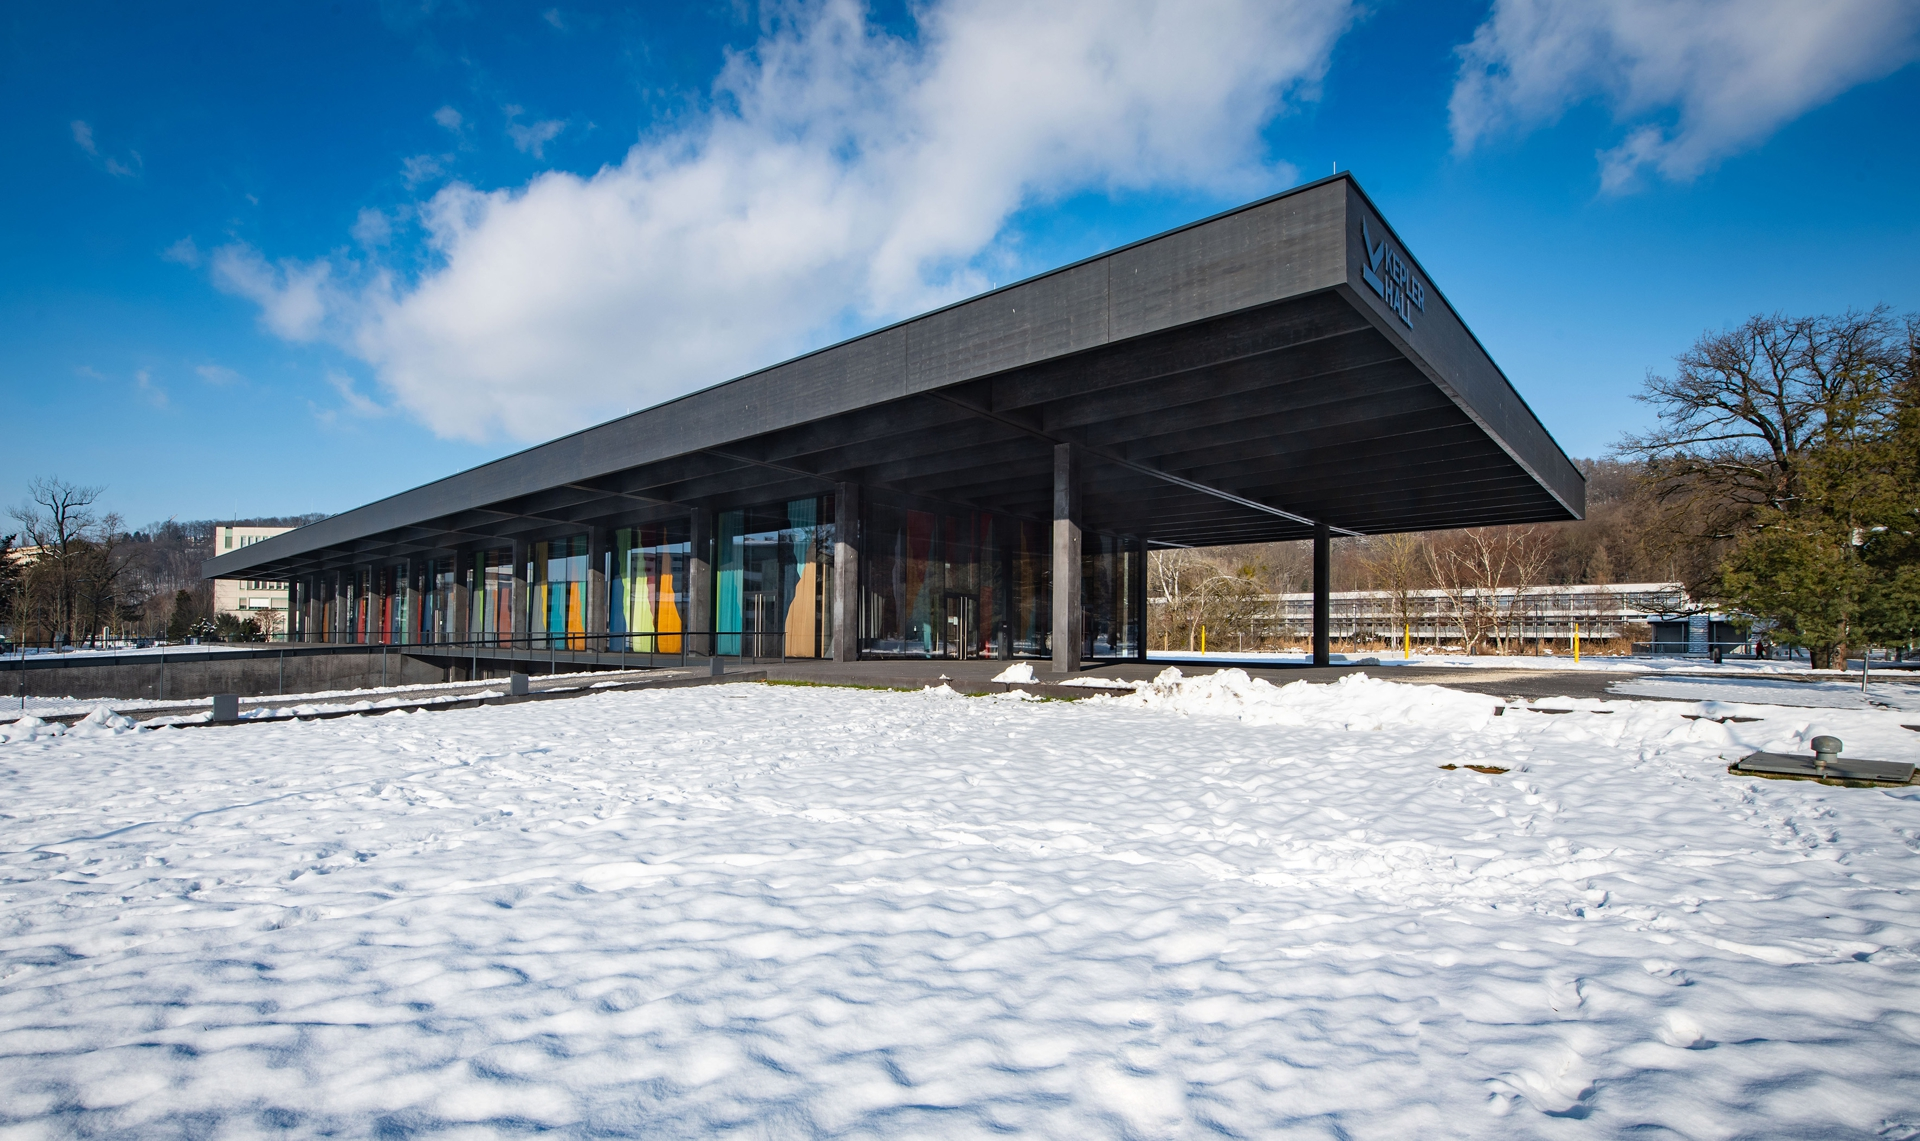
\includegraphics[width=\paperwidth]{images/jku_keplerhall_winter.jpg}}
        \setbeamercolor{normal text}{fg=white}
        \usebeamercolor[fg]{normal text}
        \begin{frame}[containsverbatim,plain]
            \frametitle{Background Image}

            You can add a full screen background image to a slide. The aspect ratio of the picture should match the presentation. To fill the whole screen you might use \verb|height=\paperheight|, but the result might be distorted~\ldots

            \bigskip
            \setbeamercolor{thisboxcolor}{bg=white,fg=black}
            \pgfsetfillopacity{0.6}
            \begin{beamercolorbox}[wd=\linewidth,dp=0ex,vmode]{thisboxcolor}
                \pgfsetfillopacity{1.0}
                \begin{lstlisting}[language={[LaTeX]TeX},numbers=none,xleftmargin=0.5em,xrightmargin=0.5em]
\begingroup
\usebackgroundtemplate{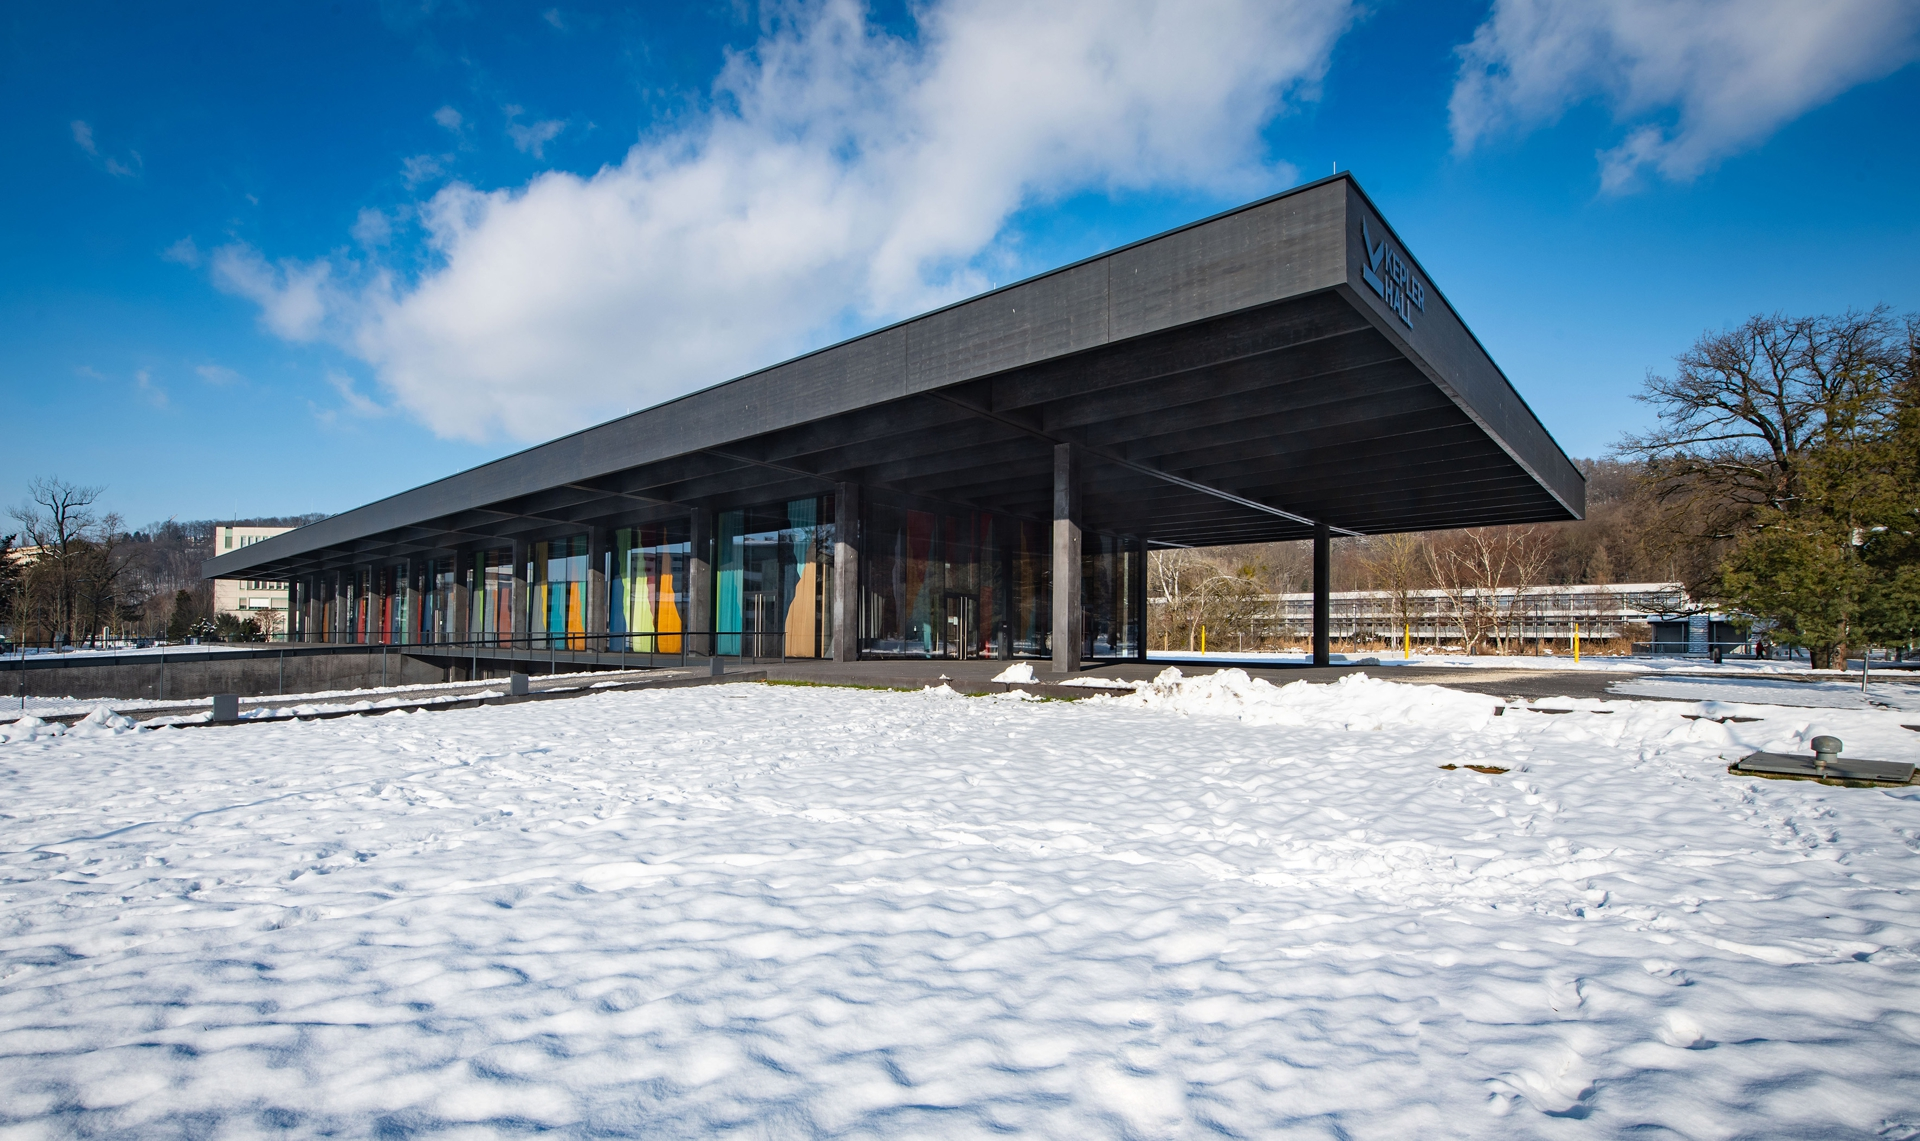
\includegraphics[width=\paperwidth]{images/jku_keplerhall_winter.jpg}}
\setbeamercolor{normal text}{fg=white}
\usebeamercolor[fg]{normal text}
\begin{frame}[plain]
\frametitle{Space for your frame title.}

Space for your frame body.
\end{frame}
\endgroup
\end{lstlisting}
            \end{beamercolorbox}
        \end{frame}
        \endgroup


        \begin{frame}[containsverbatim,plain]
            \frametitle{Title Image Slide}

            Use \verb|\imageframe[<mode options>]{<title>}{<subtitle>}{<graphic>}| to display a title image frame. That is a full screen image with a title sidebar.

            \begin{lstlisting}[language={[LaTeX]TeX},numbers=none]
\imageframe{%
    This is an image frame.
}{%
    With a subtitle.
}{%
    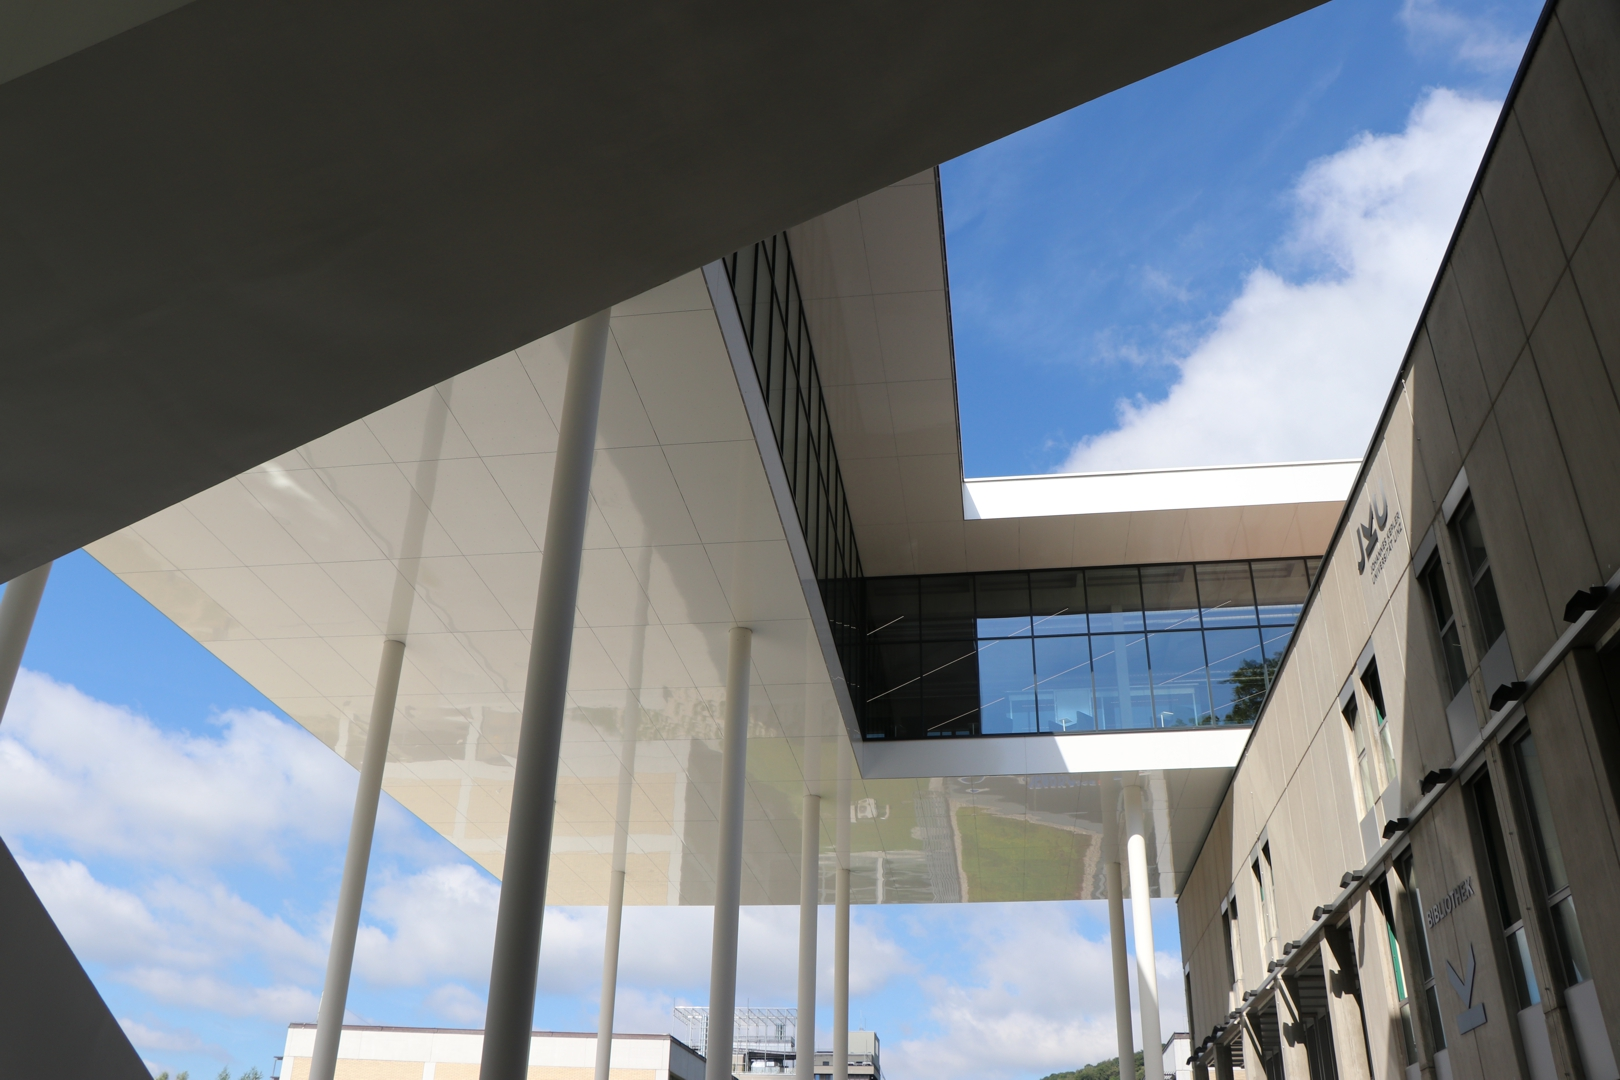
\includegraphics[height=\paperheight]{images/jku_learningcenter.jpg}
}
\end{lstlisting}

            The optional argument ``\textverb{<mode options>}'' may be any of the color mode options that can be used for the \verb|\maketitle| command (see slide~\ref{advanced-title-slides}).
        \end{frame}

        \imageframe[dark]{%
            This is a title image frame.
        }{%
            With a subtitle.
        }{%
            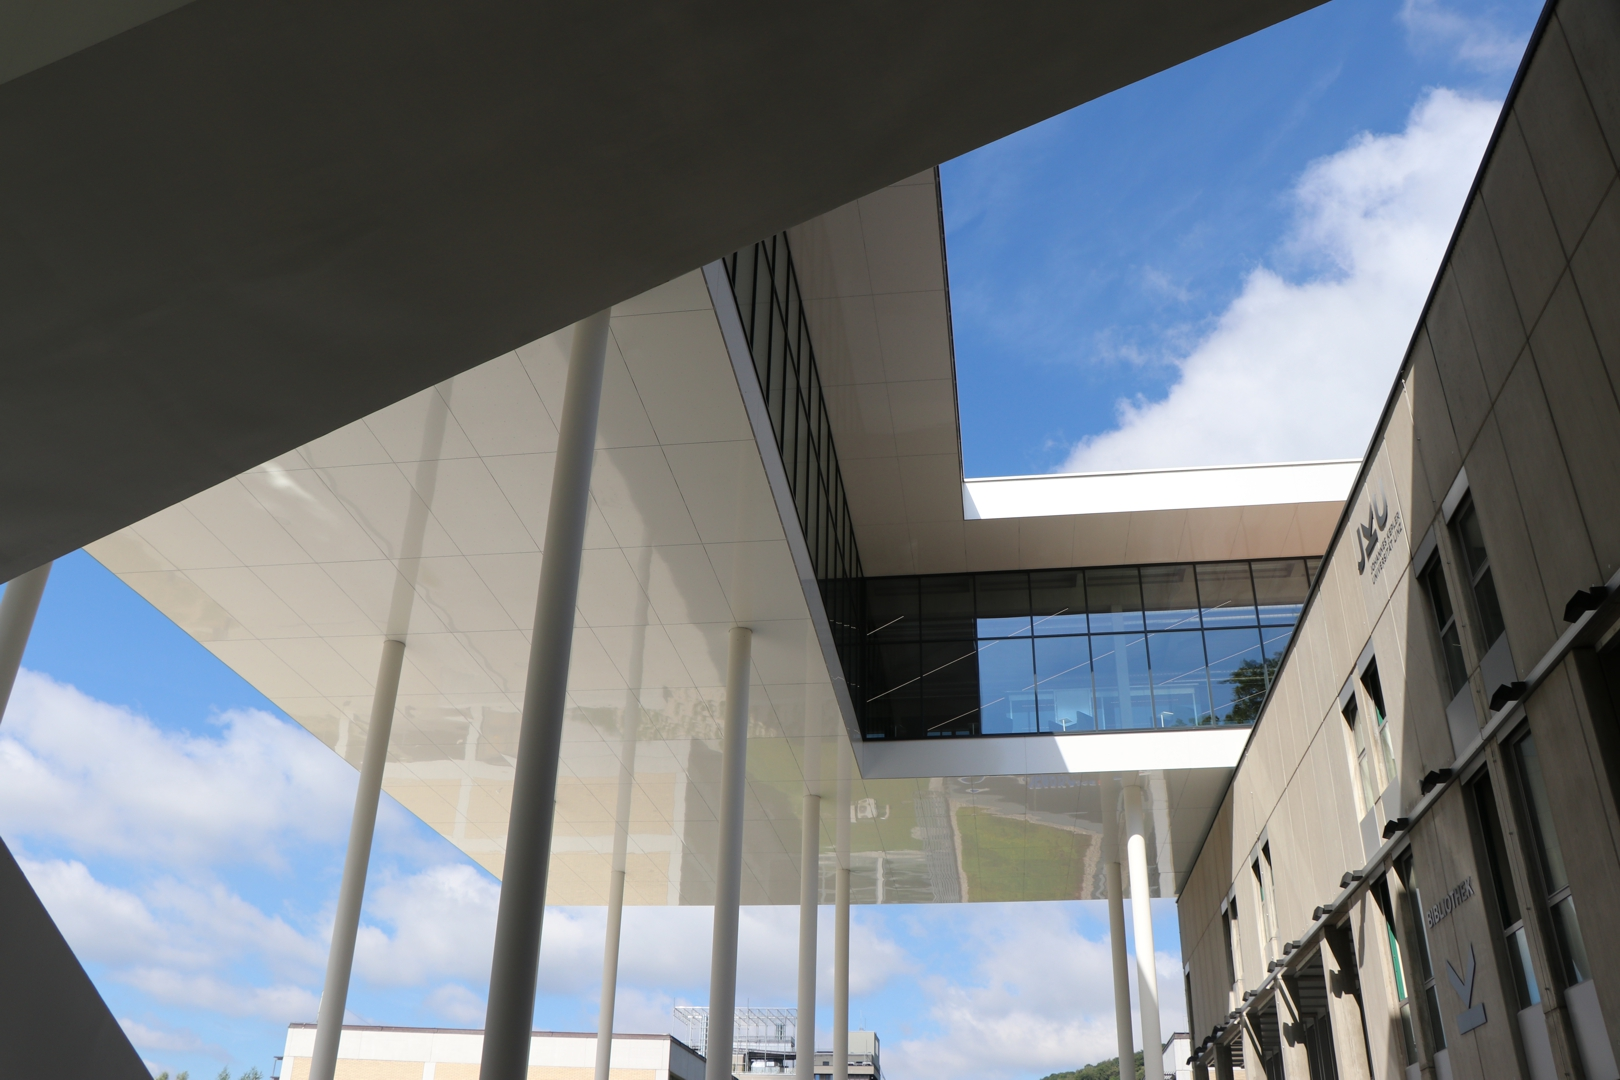
\includegraphics[height=\paperheight]{images/jku_learningcenter.jpg}
        }

        \imageframe[dark,MED]{%
            This is a title image frame.
        }{%
            For the MED faculty.
        }{%
            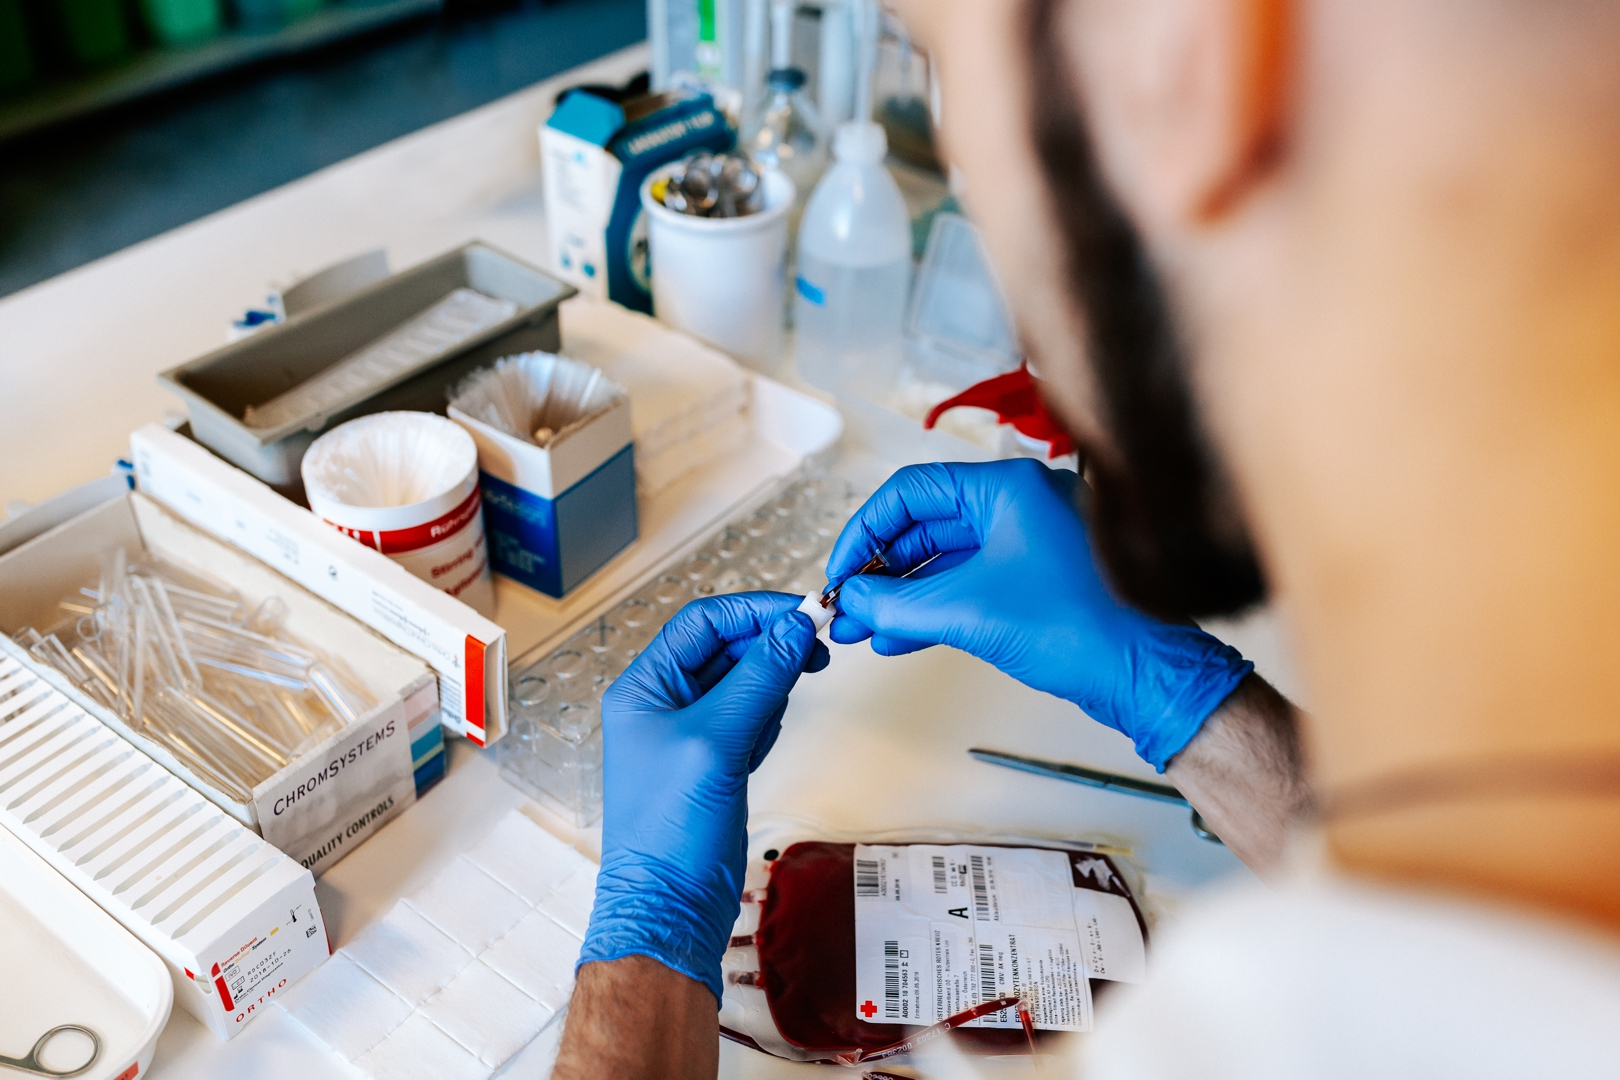
\includegraphics[height=\paperheight]{images/jku_med_image.jpg}
        }


        \begin{frame}[containsverbatim]
            \frametitle{Logo Slides}

            Use \verb|\jkulogo[<mode options>]| to display a logo slide. That is a slide with only the JKU logo centered on it. This slide is well suited as a final slide in your presentation.

            Again, the optional argument ``\textverb{<mode options>}'' may be any of the color mode options that can be used for the \verb|\maketitle| command (see slide~\ref{advanced-title-slides}), e.g.
            \begin{itemize}
                \item \textverb{\string\jkulogo}
                \item \textverb{\string\jkulogo[light]}
                \item \textverb{\string\jkulogo[dark]}
                \item \textverb{\string\jkulogo[SOWI,dark]}
                \item \textverb{\string\jkulogo[gray]}
                \item \textverb{\string\jkulogo[black]}
            \end{itemize}
        \end{frame}

        \jkulogo
        \jkulogo[light]
        \jkulogo[dark]
        \jkulogo[SOWI,dark]
        \jkulogo[gray]
        \jkulogo[black]


        \begin{frame}[containsverbatim]
            \frametitle{Switching Color Mode and Scheme}

            Just like switching the color mode and scheme for a specific special slide, you can also switch the color mode for the remaining part of the presentation. This may be useful if you want to create a presentation with parts focusing on more than one faculty.

            Use \verb|\setcolormode[<mode options>]| to change the color mode.
        \end{frame}


        \begin{frame}[containsverbatim,allowframebreaks]
            \frametitle{Contact Information Slide}

            Use \verb|\contactframe[<mode options>]{<name>}{<affiliation>}{<contact info>}{<ack>}| to display a contact information frame.
            \begin{lstlisting}[language={[LaTeX]TeX},numbers=none]
\contactframe{Johanna Kepler}{Institute of Networks and Security}{%
    \contactphone{+43 732 2468-XXXX}
    \contactmail{firstname.lastname@jku.at}
    \contactweb[https://www.jku.at/ins]{jku.at/ins}
}{%
    This work is funded by XYZ.
}
\end{lstlisting}
            The optional argument ``\textverb{<mode options>}'' may be any of the color mode options that can be used for the \verb|\maketitle| command (see slide~\ref{advanced-title-slides}).

            \framebreak
            The contact info field may contain a combination of the following commands:
            \begin{itemize}
                \item \verb|\contactaddress{address}|: adds an address/place
                \item \verb|\contactphone{number}|: adds a phone number
                \item \verb|\contactfax{number}|: adds a fax number
                \item \verb|\contactmail{e-mail address}|: adds an e-mail address
                \item \verb|\contactweb[real url]{display url}|: adds a URL
                \item \verb|\contactother[icon]{contact info}|: adds an arbitrary contact info entry, use \verb|\fa...| (from \verb|fontawesome5| package) as icons
                \item \verb|\contactnewline|: adds an empty line
            \end{itemize}
        \end{frame}

        \contactframe[dark]{%
            Johanna Kepler
        }{%
            Institute of Networks and Security
        }{%
            \contactphone{+43 732 2468-XXXX}
            \contactmail{firstname.lastname@jku.at}
            \contactweb[https://www.jku.at/ins]{jku.at/ins}
        }{%
            This work is funded by XYZ.
        }

        \contactframe[light]{%
            Johanna Kepler
        }{%
            Institute of Networks and Security
        }{%
            \contactphone{+43 732 2468-XXXX}
            \contactmail{firstname.lastname@jku.at}
            \contactweb[https://www.jku.at/ins]{jku.at/ins}
        }{%
            This work is funded by XYZ.
        }






        \section{General \LaTeX/Beamer Features}


        \begin{frame}
            \frametitle{Environments}

            Standard \LaTeX-beamer defines several environments like
            \begin{quote}
                theorem, corollary, fact, lemma, problem, solution, definition, definitions, example, and examples.
            \end{quote}

            \begin{definition}[Monoid]
                We call $(M,\circ)$ a \emph{monoid} if and only if
                \begin{gather*}
                    \forall a,b,c\in M:\quad(a\circ b)\circ c = a\circ(b\circ c) \tag{associativity}\\
                    \exists e\in M \;\forall a\in M:\quad a\circ e = e\circ a= a \tag{neutral element}
                \end{gather*}
            \end{definition}
        \end{frame}

        \begin{frame}
            \frametitle{Environments}

            \begin{theorem}[Fundamental Theorem of \ldots]
                Let $(M,+)$ be a monoid. Then \ldots
            \end{theorem}

            \begin{proof}
                Let $M$ be an arbitrary set. We then show \ldots
            \end{proof}

            \begin{example}
                Put an example here.
            \end{example}
        \end{frame}


        \begin{frame}[fragile]
            \frametitle{Self-defined Environments}

            You also can define your own environments:
            \begin{lstlisting}[language={[LaTeX]TeX},numbers=none]
\newtheorem{idea}[theorem]{Idea}

\begin{idea}[My own idea]
Here is a self-defined environment
\end{idea}

\theoremstyle{definition}
\newtheorem{defi}[theorem]{My Definition}

\begin{defi}
Test
\end{defi}
\end{lstlisting}
        \end{frame}

        \newtheorem{idea}[theorem]{Idea}
        \theoremstyle{definition}
        \newtheorem{defi}[theorem]{My Definition}
        \theoremstyle{example}
        \newtheorem{ex}[theorem]{My Example}

        \begin{frame}[fragile]
            \frametitle{Self-defined Environments}

            \begin{idea}[My own idea]
                Here is a self-defined environment
            \end{idea}

            \begin{defi}
                Test
            \end{defi}

            \begin{ex}
                Test
            \end{ex}
        \end{frame}


        \begin{frame}[fragile]
            \frametitle{Custom Blocks}
            \begingroup
            \setbeamercolor{block title}{fg=white,bg=jkuBlue}
            \begin{block}{Blue block}
                Using the theme colors to generate colored blocks.
            \end{block}
            \endgroup

            \begin{lstlisting}[language={[LaTeX]TeX},numbers=none]
\begingroup
\setbeamercolor{block title}{fg=white,bg=jkuBlue}
\begin{block}{Blue block}
Use the theme colors to generate colorful blocks.
\end{block}
\endgroup
\end{lstlisting}
        \end{frame}


        \begin{otherlanguage}{ngerman}
            \begin{frame}[fragile]
                \frametitle{Language}
                \begin{itemize}
                    \item Use the \textverb{otherlanguage} environment to temporarily change the document language in your presentation.
                    \item Changing the document language to \textverb{german} (or better \textverb{ngerman}) also changes the language in logos and the imprint on title pages and in footers.
                \end{itemize}

                \begin{lstlisting}[language={[LaTeX]TeX},numbers=none]
\begin{otherlanguage}{ngerman}

\end{otherlanguage}
\end{lstlisting}
            \end{frame}
        \end{otherlanguage}


        \begin{frame}[label=handout]
            \frametitle{Producing Handouts}

            \begin{itemize}
                \item You can generate a ``handout'' version of your presentation with the class option \textverb{handout}.
                \item Section slides and logo slides will be suppressed.
                \item Overlays will be flattened into single pages.
                \item Slide numbering will still match the numbering in the non-handout version.
            \end{itemize}
        \end{frame}


        \section{Ending the Presentation}

        \begin{frame}
            \frametitle{Thank You Thank You Thank You Thank You Thank You Thank You Thank You Thank You Thank You}

            You see, btw., the slide title can run over several lines \ldots

            \bigskip
            \begin{alertblock}{Please \ldots}
                \ldots\ refrain from putting an extra slide at the end saying ``\alert{Thank you for your attention}''. This is really annoying~\cite{schultz,karol}. You can say ``Thank you'' anyway, it need not be written. Instead, you can put a nice \textverb{\string\jkulogo} as the final slide!
            \end{alertblock}

        \end{frame}


        \begin{frame}[allowframebreaks]{References}
            %\setbeamerfont{bibliography item}{size={\footnotesize}}
            %\AtNextBibliography{\footnotesize}
            \printbibliography
        \end{frame}


        \begin{frame}
            \frametitle{JKU Theme Information}

            This a beamer theme for \href{https://www.jku.at/}{Johannes Kepler University Linz, Austria}.

            \bigskip
            \begin{exampleblock}{Want to report a bug? Want to request improvements?}
                You are always welcome to suggest improvements via the official repository at \url{https://github.com/michaelroland/jku-templates-presentation-latex}.
            \end{exampleblock}
        \end{frame}


        \jkulogo

    \fi
\end{comment}
\end{document}
\endinput
